%!LW recipe=latexmk (latexmkrc)
%==============================================================================
% ICLR 2026 conference paper
% Based on the official ICLR 2026 template (see reference/ for the unmodified
% formatting instructions). Build: latexmk main.tex   (output -> ../build-iclr)
%
% Conference requirements (ICLR 2026):
%   - Main text: max 9 pages at submission (10 pages for rebuttal/camera-ready).
%     References and appendices do not count toward the limit.
%   - Double-blind: keep \iclrfinalcopy commented out for submission; the style
%     file then replaces the author block with "Anonymous authors" automatically.
%   - Citations via natbib: \citet{} in-sentence, \citep{} in parentheses.
%==============================================================================

\documentclass{article} % For LaTeX2e
\usepackage{iclr2026_conference,times}

% Optional math commands from https://github.com/goodfeli/dlbook_notation.
\input{math_commands.tex}

\usepackage{hyperref}
\usepackage{url}
\usepackage{graphicx}
\usepackage{subcaption}
\graphicspath{{img/}}
\usepackage{wrapfig}

% For the algorithm box in the method section:
%\usepackage{algorithm}
%\usepackage{algorithmic}

% TODO Set the paper title
\title{BVER: Bi-directional incremental Voronoi-biased Exploration curriculum for Reinforcement learning}
    
% Authors must not appear in the submitted version. They are hidden
% as long as the \iclrfinalcopy macro remains commented out below.
% Non-anonymous submissions will be rejected without review.
\author{Juri Pfammatter, Victor Klemm, Kaixian Qu, Clemens Schwarke \& Marco Hutter \\
Robotic Systems Lab\\
ETH Z\"urich\\
Z\"urich, Switzerland \\
\texttt{jpfammatter@ethz.ch,}\\
\texttt{\{vklemm, kaixqu, clemens, mahutter\}@leggedrobotics.com} \\
}

\iclrfinalcopy{} % Uncomment for camera-ready version, but NOT for submission.

\begin{document}

\maketitle

\begin{abstract}
    Goal-conditioned reinforcement learning in sparse-reward, long-horizon tasks is bottlenecked by exploration: from the default start, a policy almost never sees the success signal.
    Existing automatic curricula are anchored at a single point: they move only one endpoint, proposing goals for a fixed start or start states for a fixed goal, or grow both from one seed region, so the target is only ever approached from one direction.
    We propose BVER, which borrows from sampling-based motion planning.
    Two sets of physically valid states are expanded by short random walks, seeded with an RRT-style Voronoi bias toward unexplored task space, and filtered to the frontier of the policy's current ability, while a single goal-conditioned policy trains on both.
    Unlike prior curricula, BVER grows a start-state frontier outward from the goal and a goal frontier outward from the start simultaneously, and an RRT-Connect-style step connects them, so the target task is approached from both ends at once.
    Learning from a binary reward alone, with no reference motions, hand-designed curricula, or shaping, BVER solves quadrupedal box climbing under wide start, goal, and yaw variation, is the most sample-efficient demonstration-free method tested, and extends to sparse-reward maze navigation and manipulation tasks.

    The project website, videos and code are available at \url{https://juripfammatter.com/html/bver_demo/bver.html} (replace with anonymous project website for submission).
    %TODO: create anonymous project website for submission
\end{abstract}

\section{Introduction}\label{sec:introduction}

Many robotic tasks are posed as reaching a goal: a quadruped that should climb onto a box is rewarded for standing on top of it, not for how it gets there. Under such a sparse reward and a long horizon, a policy started from the initial state distribution essentially never reaches the goal and therefore receives no learning signal~\citep{florensa2017reverse}. Policy gradient methods such as PPO~\citep{schulman2017proximal} perform a local search that improves the policy from the returns of the trajectories it currently generates, and a reward that none of these trajectories collects cannot guide it.

In quadrupedal locomotion, terrain curricula with dense rewards~\citep{rudin2022learning, lee2020learning}, reference motions from trajectory optimization~\citep{fuchioka2023opt}, and hand-designed curricula~\citep{atanassov2024curriculum} supply the missing signal, achieving good performance on a wide range of difficult terrains and tasks. However, each requires a demonstration or engineering specific to one task, and curiosity-driven exploration~\citep{schwarke2023curiosity} adds rewards that the task itself does not provide.

Automatic curriculum learning replaces this design effort with intermediate tasks generated during training~\citep{narvekar2020curriculum, portelas2020automatic}. Start-state and goal curricula address goal-conditioned tasks directly by shortening the task from one of its two ends: start-state curricula begin closer to the goal, with start states taken from a reference trajectory~\citep{peng2018deepmimic, resnick2018backplay} or from random walks outward from the goal~\citep{florensa2017reverse}, and goal curricula keep the start fixed and propose intermediate goals~\citep{florensa2018automatic, ren2019exploration, cho2023outcome}. Both typically expand from one end only, so the curriculum has to carry its frontier across the entire distance to the end that stays fixed. The policy, in turn, sees the target task from one side, reaching the goal from many starts or many goals from the start, but not both. In addition, the random walks of reverse curriculum generation~\citep[RC;][]{florensa2017reverse} are seeded without regard to coverage, so nothing promotes the frontier into unvisited task space or toward the initial state distribution.

Two mechanisms from sampling-based motion planning address exactly this. Rapidly-exploring random trees~\citep[RRT;][]{lavalle2001randomized} extend the vertex nearest to a uniform sample of the space, so growth is biased toward large unexplored regions (the Voronoi bias), and RRT-Connect~\citep{kuffner2000rrt} grows one tree from the start and one from the goal and extends each toward the other until they meet. BVER (Bidirectional incremental Voronoi-biased Exploration curriculum for Reinforcement learning) transfers both to curriculum generation. It grows start states outward from the goal by random walks (the backwards expansion) and goals outward from the initial state distribution in the same way (the forwards expansion), connects the two sets, and trains a single goal-conditioned policy on both intermediate starts and goals. This creates a curriculum whose proposed tasks are both at the right difficulty and promote coverage of the task space, and thus of the target task.

We evaluate BVER with sparse rewards in three domains: point-mass mazes, simulated quadrupedal box climbing, and a Tower of Hanoi manipulation experiment. In all three, PPO rarely or never finds a solution without a curriculum, and BVER converges faster than every reference-free curriculum we compare against on all but the simplest maze. On box climbing, the resulting policy holds up under start, goal, and yaw variations on which the other curricula fail. Ablations on the navigation, locomotion and manipulation experiments show that expanding from both ends outperforms either direction alone.

Our contributions are:
\begin{itemize}[leftmargin=16pt, topsep=0.0em]
    \item An expansion mechanism carrying the Voronoi bias of RRT and the connect step of RRT-Connect over to curriculum generation, growing each frontier toward unexplored task space and toward the other frontier.
    \item An automatic start-goal curriculum for goal-conditioned RL with sparse rewards and long horizons that expands bidirectionally to propose starts and goals to train one policy on both, without reference motions, shaped rewards, or a hand-designed curriculum.
    \item An evaluation against reference-free and reference-based curricula on point-mass navigation, high-dimensional quadrupedal locomotion, and manipulation with sparse rewards and long horizons, and ablations BVER's components.
\end{itemize}
In total, we evaluate on thirteen experiments: three point-mass mazes, four box climbing variants, a Tower of Hanoi manipulation, the three-route terrain, and four scanned real-world terrains.

\section{Related work}\label{sec:related_work}

% ~0.75-1 page, partitioned into 3-4 labeled thematic blocks.
% Each block MUST close with an explicit delta sentence:
%   ``In contrast, our method \ldots'' / ``\ldots is unique to our approach.''
\paragraph{Automatic curriculum learning:}
Automatic curriculum learning (ACL) adapts the sequence of training tasks to the capabilities of the learner during training~\citep{narvekar2020curriculum, portelas2020automatic}. \citet{portelas2020automatic} sort ACL methods for data collection by what they control: the initial state, the reward function, the goal, the environment, or the opponent. Environment curricula sample the parameters of a procedural generator by absolute learning progress~\citep{portelas2020teacher}, replay previously seen levels prioritized by the magnitude of their value loss~\citep{jiang2021prioritized}, or widen the ranges of domain randomization once performance at their boundary exceeds a threshold~\citep{akkaya2019solving}; all of them assume an environment that can be parameterized or regenerated. Reward curricula such as RND~\citep{burda2018exploration} add as intrinsic reward the error of a network that predicts the features of a fixed random network, which by its authors' own account handles local exploration but not global exploration over long horizons. BVER controls neither environment nor reward and changes only where an episode starts and which goal it is given.

\paragraph{Start-state and goal curricula:}
Reverse curriculum generation~\citep[RC;][]{florensa2017reverse} grows start states outward from a given goal state with short rollouts of random actions and keeps those from which the current policy reaches the goal sometimes but not always; it needs no demonstrations, only a simulator that resets to arbitrary states and one goal state. BaRC~\citep{ivanovic2019barc} replaces the random rollouts with backward reachable sets computed from an approximate dynamics model, so that the frontier grows in every direction the dynamics allow. Reference state initialization~\citep[RSI;][]{peng2018deepmimic} samples the start state uniformly from a reference motion, Backplay~\citep{resnick2018backplay} moves a window of start states backward along a single demonstration on a fixed schedule, and RFCL~\citep{tao2024reverse} runs a reverse curriculum per demonstration and then prioritizes initial states of the task by success rate; all three vary only the start state and rely on demonstrations. Goal curricula generate goals for the task's own initial state distribution: GoalGAN~\citep{florensa2018automatic} trains a generator to propose goals of intermediate difficulty, HGG~\citep{ren2019exploration} selects achieved states from the replay buffer by their Wasserstein distance to the target task distribution and their value, and OUTPACE~\citep{cho2023outcome} selects them by temporal distance from the initial distribution, uncertainty, and progress toward given outcome examples. In contrast, BVER grows intermediate starts and intermediate goals at the same time, biases both toward unexplored task space, and connects the two sets, which, unlike RC and BaRC, drives the frontiers toward the target task. Combining start-state generation with goal generation, by analogy to RRT-Connect, is what \citet{florensa2017reverse} proposed as future work.

\paragraph{Sampling-based planning:}
A rapidly-exploring random tree~\citep{lavalle2001randomized} extends the vertex nearest to a random sample of the space; since a vertex is selected with probability proportional to the area of its Voronoi region, the tree is biased to explore rapidly~\citep{kuffner2000rrt}. RRT-Connect~\citep{kuffner2000rrt} grows two trees from the start and the goal and tries to connect them. BVER seeds its random walks with the same Voronoi bias and connect step, growing a curriculum rather than a path.

\paragraph{Quadrupedal Locomotion:}

Current state-of-the-art quadrupedal locomotion methods do not train on sparse rewards, long-horizon tasks and often rely on reference motions or hand-designed curricula.
For example, \citet{rudin2022learning} utilize a game-inspired terrain curriculum with dense rewards.\ \citet{lee2020learning} replace the game-inspired curriculum with an adaptive particle filter based parametric terrain curriculum.
\citet{fuchioka2023opt} use trajectory optimization to find a solution and then train with RSI~\citep{peng2018deepmimic} as an initialization curriculum.
\citet{atanassov2024curriculum} hand-design a three-stage curriculum for jumping and initialize the first stage at random heights and upward velocities, a form of RSI without a reference trajectory, which they find necessary to learn jumping in place.
\citet{schwarke2023curiosity} learn a quadrupedal loco-manipulation task on sparse rewards by extending RND~\citep{burda2018exploration} with a curiosity state.
Our method differs from these as it learns on sparse rewards directly, without reference motions, hand-designed curricula and without additional rewards.
\section{Preliminaries}\label{sec:preliminaries}

% ~0.4 page total.
% Notation (agreed 2026-09-02): P transition kernel, H episode horizon,
% \mathcal{T} task space, \rho_0 initial state distribution, g^\star target goal,
% \epsilon goal tolerance.
% When porting the pseudocode: p_0 -> \rho_0, G -> g^\star, T_B unchanged.

\subsection{Goal-Conditioned Markov Decision Process}\label{sec:problem_formulation}

We model the task as a goal-augmented Markov decision process (GA-MDP)~\citep{liu2022goal} with state space $\mathcal{S}$, action space $\mathcal{A}$, transition kernel $P$, discount factor $\gamma$, initial state distribution $\rho_0$, and goal space $\mathcal{G}$.
A known mapping $\phi: \mathcal{S} \to \mathcal{G}$ projects a state onto the goal it achieves~\citep{andrychowicz2017hindsight}, and a goal $g$ is reached in state $s$ if $\lVert \phi(s) - g \rVert \le \epsilon$ for a tolerance $\epsilon$.
The reward is sparse and binary: the agent receives $+1$ in every step in which the goal is reached and $0$ otherwise. Episodes have a fixed horizon $H$ and do not terminate when the goal is reached.

The agent acts with a goal-conditioned policy $\pi_\theta(a \mid s, g)$~\citep{schaul2015universal}, trained with PPO~\citep{schulman2017proximal}.
%  in massively parallel simulation~\citep{rudin2022learning}.
We denote by $R(\tau, g)$ the discounted return of a rollout $\tau$ under goal $g$. Because the reward keeps accruing at the goal, the return measures how quickly and how reliably the policy reaches the goal and stays there, rather than a binary success.
The \emph{target task} is to reach a single target goal $g^\star \in \mathcal{G}$ from the initial state distribution $\rho_0$, and the learning objective is to maximize the expected return on this task.

\subsection{Curriculum}\label{sec:curriculum}

Optimizing the target task directly fails under sparse rewards and long horizons: a randomly initialized policy essentially never reaches $g^\star$ from $\rho_0$ and thus receives no learning signal~\citep{florensa2017reverse}.
Curriculum learning instead trains on a sequence of easier tasks~\citep{narvekar2020curriculum, portelas2020automatic}. In our setting, a task is a start--goal pair, and a \emph{curriculum} decides in every training iteration which pairs the policy is trained on, based on the experience collected with the current policy~\citep{tao2024reverse}. The intermediate tasks are auxiliary, and the objective remains the target task.
A \emph{start-state curriculum} keeps the goal fixed at $g^\star$ and proposes intermediate start states~\citep{florensa2017reverse, tao2024reverse}, whereas a \emph{goal curriculum} keeps the start states drawn from $\rho_0$ and proposes intermediate goals~\citep{florensa2018automatic, ren2019exploration}. Our method does both at once: it trains one shared goal-conditioned policy on intermediate starts and intermediate goals, with the training budget split evenly between the two (Section~\ref{sec:method}).

\subsection{Assumptions}\label{sec:assumptions}

Analogous to \citet{florensa2017reverse}, we assume that the simulator can be reset to arbitrary states and simulated from them under random actions, that the initial distribution $\rho_0$ can be sampled, that one goal state $s^{g} \in \mathcal{S}$ with $\phi(s^{g}) = g^\star$ is known, and that a bounded task space $\mathcal{T}$ that contains the target task is known and can be sampled uniformly.

\section{Method}\label{sec:method}
Our method maintains finite sets of states from which the starts and goals of each training iteration are sampled uniformly at fixed ratios; $\rho^{\mathrm{S}}_e$ and $\rho^{\mathrm{G}}_e$ in Eq.~(\ref{eq:bidirectional}) are the resulting discrete distributions, and we describe the method in terms of these sets.
In the following, we first describe our method's frontier expansion mechanism for the backwards expansion, and how it extends RC's expansion mechanism to provide coverage of the task space and thus the initial distribution. Then we show how the same mechanism can be applied to the forwards expansion by substituting the start state with the goal state. Finally, we combine the two into our main contribution: a bidirectional expansion mechanism that expands the curriculum from both the start and goal states, leading to more sample-efficient and robust learning. An overview of the full method is given in Figure~\ref{fig:method} in the appendix.

% ~2-2.5 pages.
% Schematic Figure 2 (system overview) near the top: \label{fig:method}.
% One sub-headed \paragraph{} per component.
% Equations for the curriculum sampling/scoring rule.
% Algorithm box: uncomment the algorithm packages in main.tex.
% Defer hyperparameters to the appendix (Sec.~\ref{sec:appendix}).


% Overview with a figure
\subsection{Incremental Spatial Expansion}

\paragraph{Exploration:}
Similar to RC~\citep{florensa2017reverse}, we initialize the policy training with valid states obtained from simulating random actions in state space (Figure~\ref{fig:bwd_expansion_1}). After the training iteration, we separate frontier states ($R_{\min} < R < R_{\max}$) and successful states ($R_{\max} \leq R$), where $R = R(\tau, g)$ is the return of a single rollout, i.e., a one-sample estimate of $V^{\pi}(s_0, g)$, and then mix them with fixed ratios to create a balanced training set. % give better arguments here
This set contains mostly states that are neither too hard nor too easy for the current policy, and we call this set the ``mixed'' training set.

When choosing seeds for the next iteration of random walks, we add an additional criterion to enforce coverage of the task space and thus promote convergence to the initial distribution. To do so, we find the spatial frontier (Figure~\ref{fig:bwd_expansion_2}) of the explored state space by (1) sampling a set of random points uniformly from the task space $\mathcal{T}$, (2) computing the nearest neighbor in the
mixed training set for each of the sampled states, and (3) selecting these states as the seeds for the random walks (Figure~\ref{fig:bwd_expansion_3}). Similarly to the Voronoi bias inherent in Rapidly-exploring Random Trees (RRT)~\citep{lavalle2001randomized}, this biases the random walks towards unexplored areas of the task space, as they have a higher probability of being sampled than states in already explored areas.

\begin{figure}[ht]
    \centering
    \begin{subfigure}[t]{0.3\linewidth}
        \centering
        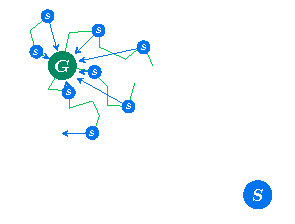
\includegraphics[width=\linewidth]{img/graphics/bwd1.pdf}
        \caption{Starting from the goal, the policy is trained on physically valid initial states ({\color{blue} blue circles}) from random walks ({\color{teal} green lines}) seeded in the goal ({\color{teal} green circle}).}\label{fig:bwd_expansion_1}
    \end{subfigure}
    \hfill
    \begin{subfigure}[t]{0.3\linewidth}
        \centering
        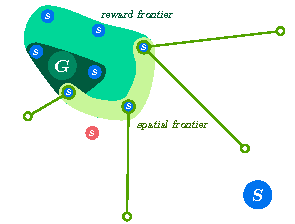
\includegraphics[width=\linewidth]{img/graphics/bwd2.pdf}
        \caption{In addition to the reward frontier ({\color{teal} light green}), the nearest neighbors of random samples from the task space determine the spatial frontier ({\color{orange} yellow circles}).}\label{fig:bwd_expansion_2}
    \end{subfigure}
    \hfill
    \begin{subfigure}[t]{0.3\linewidth}
        \centering
        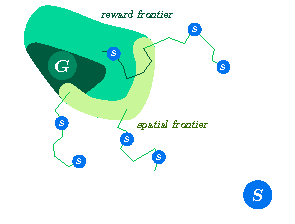
\includegraphics[width=\linewidth]{img/graphics/bwd3.pdf}
        \caption{In the next iteration, the random walks are seeded in the spatial frontier ({\color{orange} yellow circles}), leading to more efficient exploration.}\label{fig:bwd_expansion_3}
    \end{subfigure}
    \caption{Backwards expansion mechanism used in the exploration step.}\label{fig:expansion}
\end{figure}

\paragraph{Exploitation:} In addition to training the policy on unseen states in the exploration step, we also continue training on the mixed training set. This has two effects: (1) training on the reward frontier improves the policy, and (2) training on successful states mitigates catastrophic forgetting. A fixed ratio of training iterations is allocated to this step. If the policy is trained on a parallelized environment, this can be done in parallel with the exploration step, which is the case in our experiments.

Both the exploration and exploitation steps are repeated until the policy is able to solve the task from the initial distribution.


\subsection{Bidirectional Expansion}

\paragraph{Forwards expansion:}
The backwards expansion mechanism described in the previous section can be applied to the forwards expansion by substituting the start state with the goal state. The goal-conditioned policy is trained on initial states sampled from the initial distribution $\rho_0$ and goals sampled from the spatial frontier of the explored state space, i.e., $(s_0 \sim \rho_0,\, g_i)$ rather than $(s_i,\, g^\star)$. The exploration and exploitation steps are then identical, with the minor difference that the random walks are seeded in states that can be reached rather than states from which the goal can be reached.

\paragraph{Bidirectional expansion:} Combining the two expansion mechanisms, we train one shared goal-conditioned policy on both $(s_0 \sim \rho_0,\, g_i)$ and $(s_i,\, g^\star)$, with the training budget split evenly between the two expansions ($\beta = \tfrac{1}{2}$ in Eq.~(\ref{eq:bidirectional})). This leads to a diverse, incrementally expanding curriculum that covers the reachable task space from two directions. As a result, the policy is trained to reach the target goal from a wide range of start states, and to reach a wide range of goals from the initial distribution, leading to more robust policies.

\begin{wrapfigure}{r}{0.3\linewidth}
    \centering
    % \vspace{-\baselineskip} % add again if formatting changes
    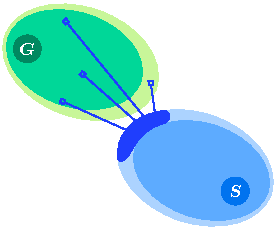
\includegraphics[width=\linewidth]{img/graphics/connect.pdf}
    \caption{The forwards expansion set can be connected to the backwards
        expansion set by sampling from the other mixed training set rather than
        random samples from the task space.}\label{fig:connect}
\end{wrapfigure}
\paragraph{Connecting the two frontiers:} In addition to the bidirectional expansion, we can also connect the two frontiers by replacing the random samples from $\mathcal{T}$ in step (1) of the spatial expansion with samples from the other frontier (Figure~\ref{fig:connect}). For example, when expanding the forwards frontier, we sample states from the mixed training set of the backwards expansion and then find their nearest neighbors in the mixed training set of the forwards expansion. As a result, the seeds of the forwards random walks lie on the side of the forwards set that faces the backwards set, and the intermediate goals grow toward the target goal $g^\star$. Symmetrically, the seeds of the backwards random walks face the forwards set, and the intermediate starts grow toward the initial distribution $\rho_0$.

% \begin{figure}[h]\label{fig:method}
%     \begin{center}
%         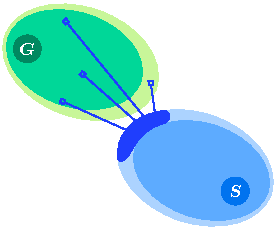
\includegraphics[width=0.3\linewidth]{img/graphics/connect.pdf}
%     \end{center}
%     \caption{The forwards expansion set can be connected to the backwards expansion set by sampling from the other mixed training set rather than random samples from the task space.}\label{fig:connect}
% \end{figure}


This leads to a more sample-efficient exploration, as each expansion moves toward the region the other expansion has already made solvable instead of spreading uniformly over $\mathcal{T}$. This is similar to the RRT-Connect algorithm~\citep{kuffner2000rrt}, where two trees are grown towards each other until they connect.

To promote both even coverage of the task space and the connection of the two frontiers, we sample from both the other frontier and the task space with a fixed ratio, the connect ratio. It balances even coverage of $\mathcal{T}$ against the connection of the two frontiers and is a hyperparameter of our method.
% ~2-2.5 pages.
\section{Experiments}\label{sec:experiments}



We conduct four experiments to answer the following research questions:
\begin{enumerate}
    \item Does our method outperform state-of-the-art curriculum learning methods on a high-dimensional quadrupedal locomotion task with sparse rewards and long horizons?
    \item Does expanding the curriculum bidirectionally improve sample efficiency and robustness compared to unidirectional expansion?
    \item Does task-space coverage-driven exploration promote more diverse learning outcomes?
    \item Does our method transfer to real-world terrains and tasks, demonstrating its practical applicability and robustness in real-world scenarios?
\end{enumerate}

%TODO: review once we have all experiments

The experiments are implemented in Isaac Lab~\citep{nvidia2025isaaclabgpuacceleratedsimulation} with the ANYmal D quadrupedal agent and the RSL-RL framework~\citep{schwarke2025rslrllearninglibraryrobotics} for training the policy with PPO~\citep{schulman2017proximal}. The following experiments use standard observation and action spaces which are detailed in Appendix~\ref{sec:appendix_obs_act}. The tasks are shown in Figure~\ref{fig:experiment_renders}. The task space $\mathcal{T}$ used for our method's random point sampling and goal definition is a 3D box defined in the $(x,y,z)$ space, i.e., $\phi(s)$ is the projection of the base position to $(x,y,z)$. We found this to be the most effective task space, as it is both convenient for goal definition and provides a simple Euclidean distance metric for the nearest-neighbor search.
\begin{figure}[h]
    \centering
    \hfill
    \begin{subfigure}[t]{0.24\linewidth}
        \centering
        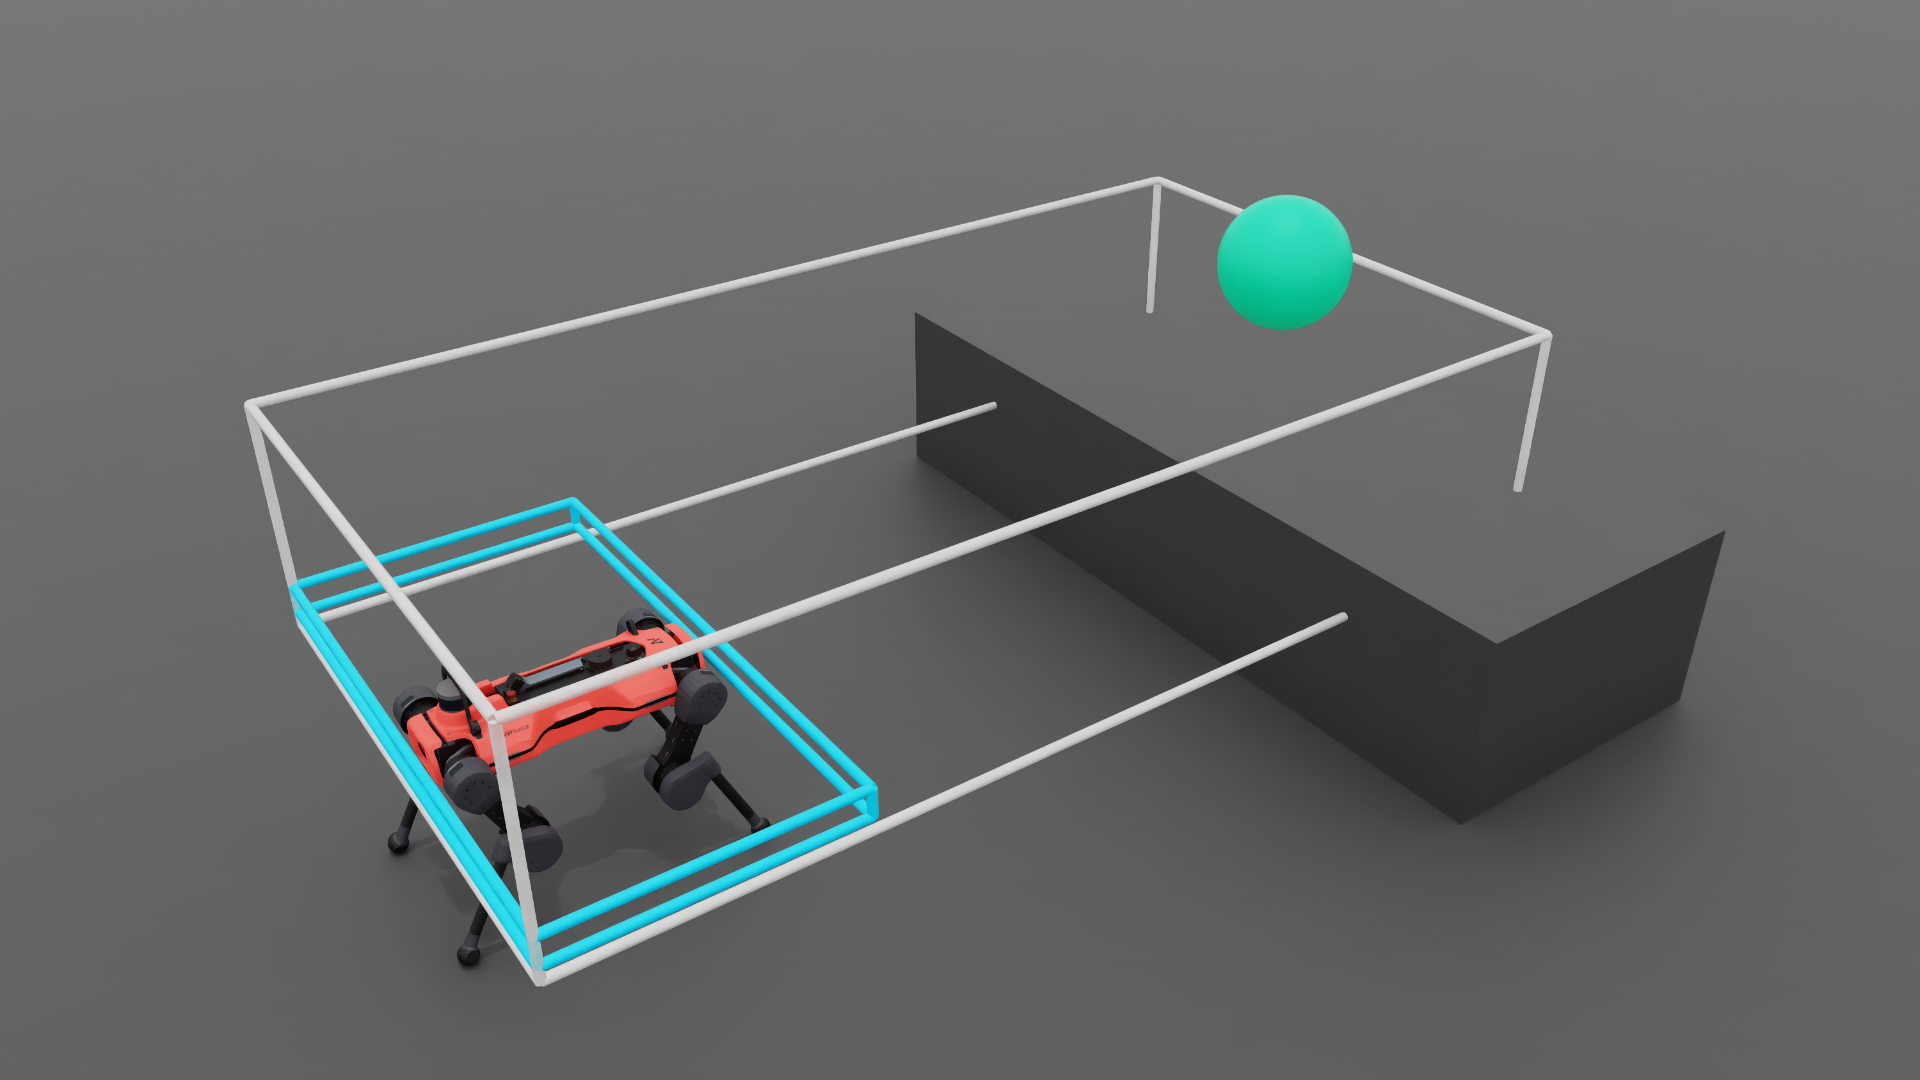
\includegraphics[width=\linewidth]{img/thumbnails/climb_box_up.png}
        \caption{Climb box up.}\label{fig:exp_renders_climb_box_up}
    \end{subfigure}
    \hfill
    \begin{subfigure}[t]{0.24\linewidth}
        \centering
        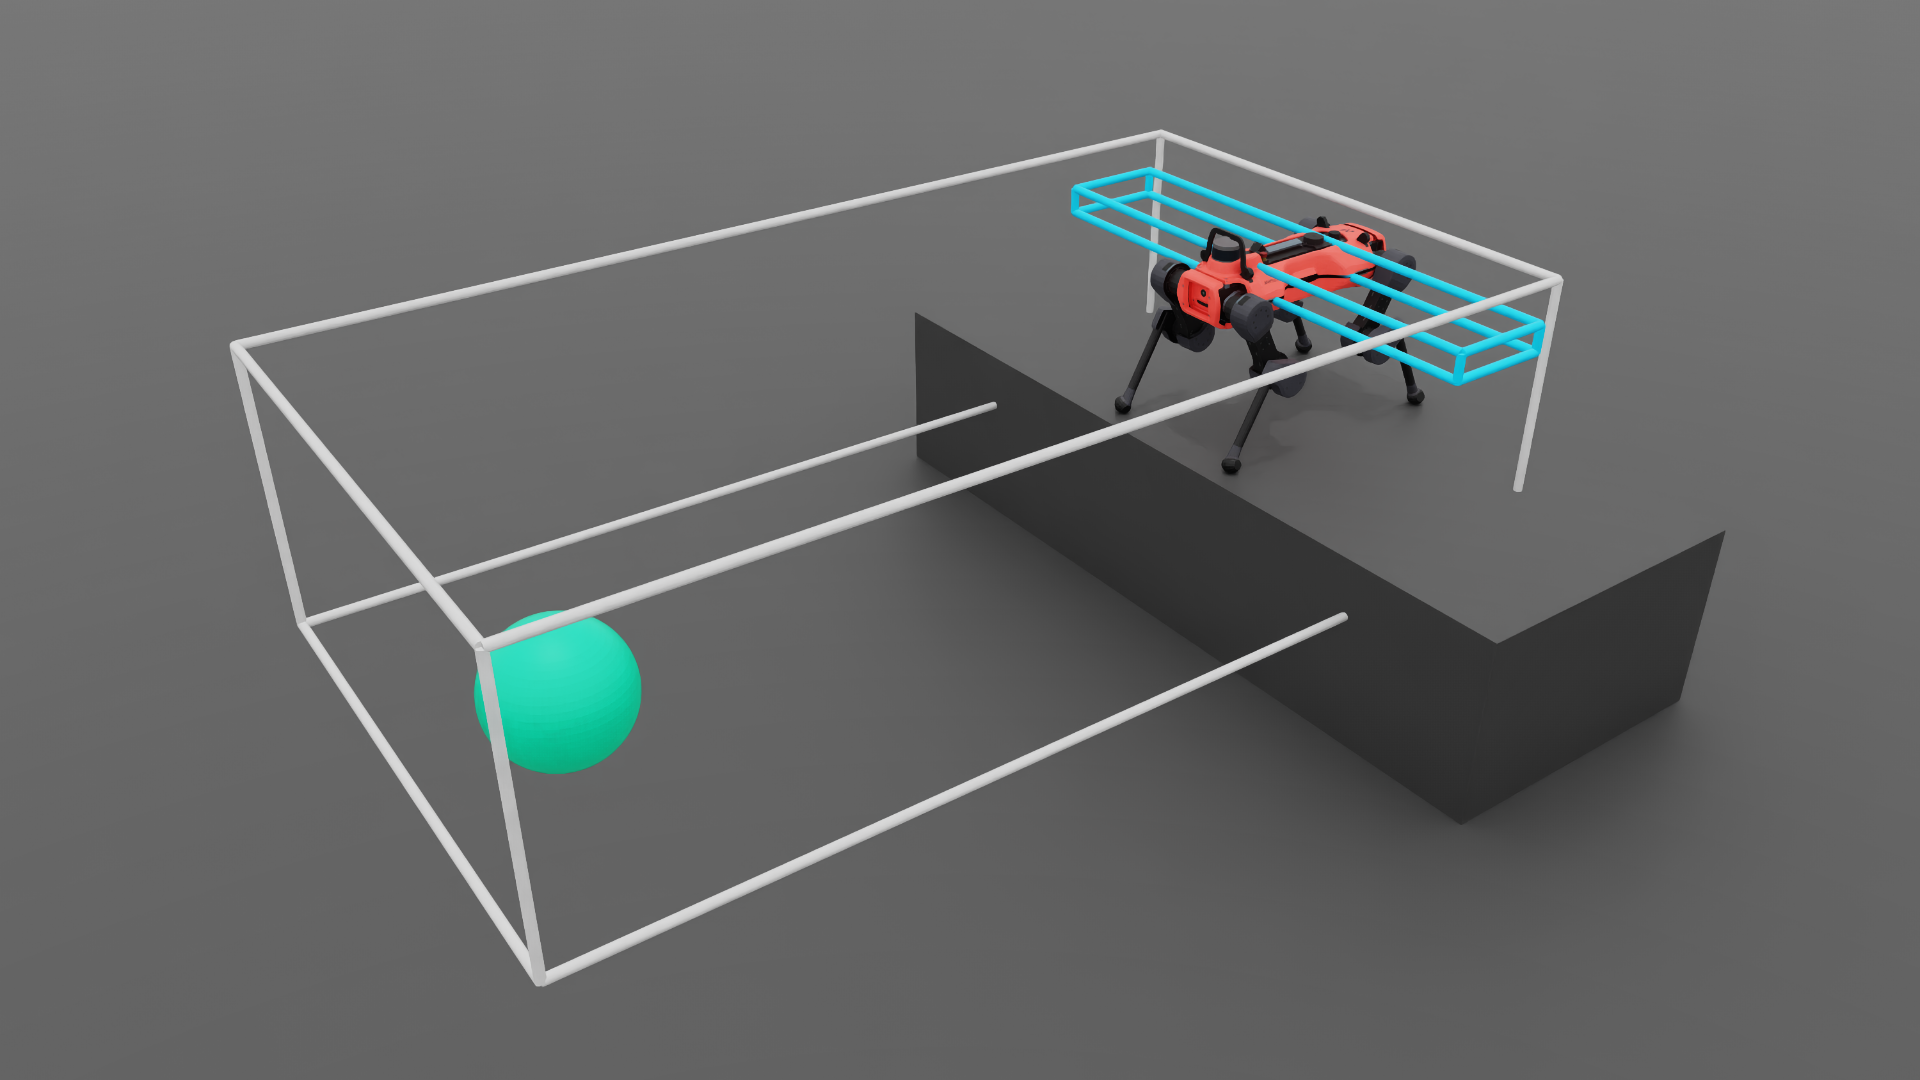
\includegraphics[width=\linewidth]{img/thumbnails/climb_box_down.png}
        \caption{Climb box down.}\label{fig:exp_renders_climb_box_down}
    \end{subfigure}
    \hfill
    \begin{subfigure}[t]{0.24\linewidth}
        \centering
        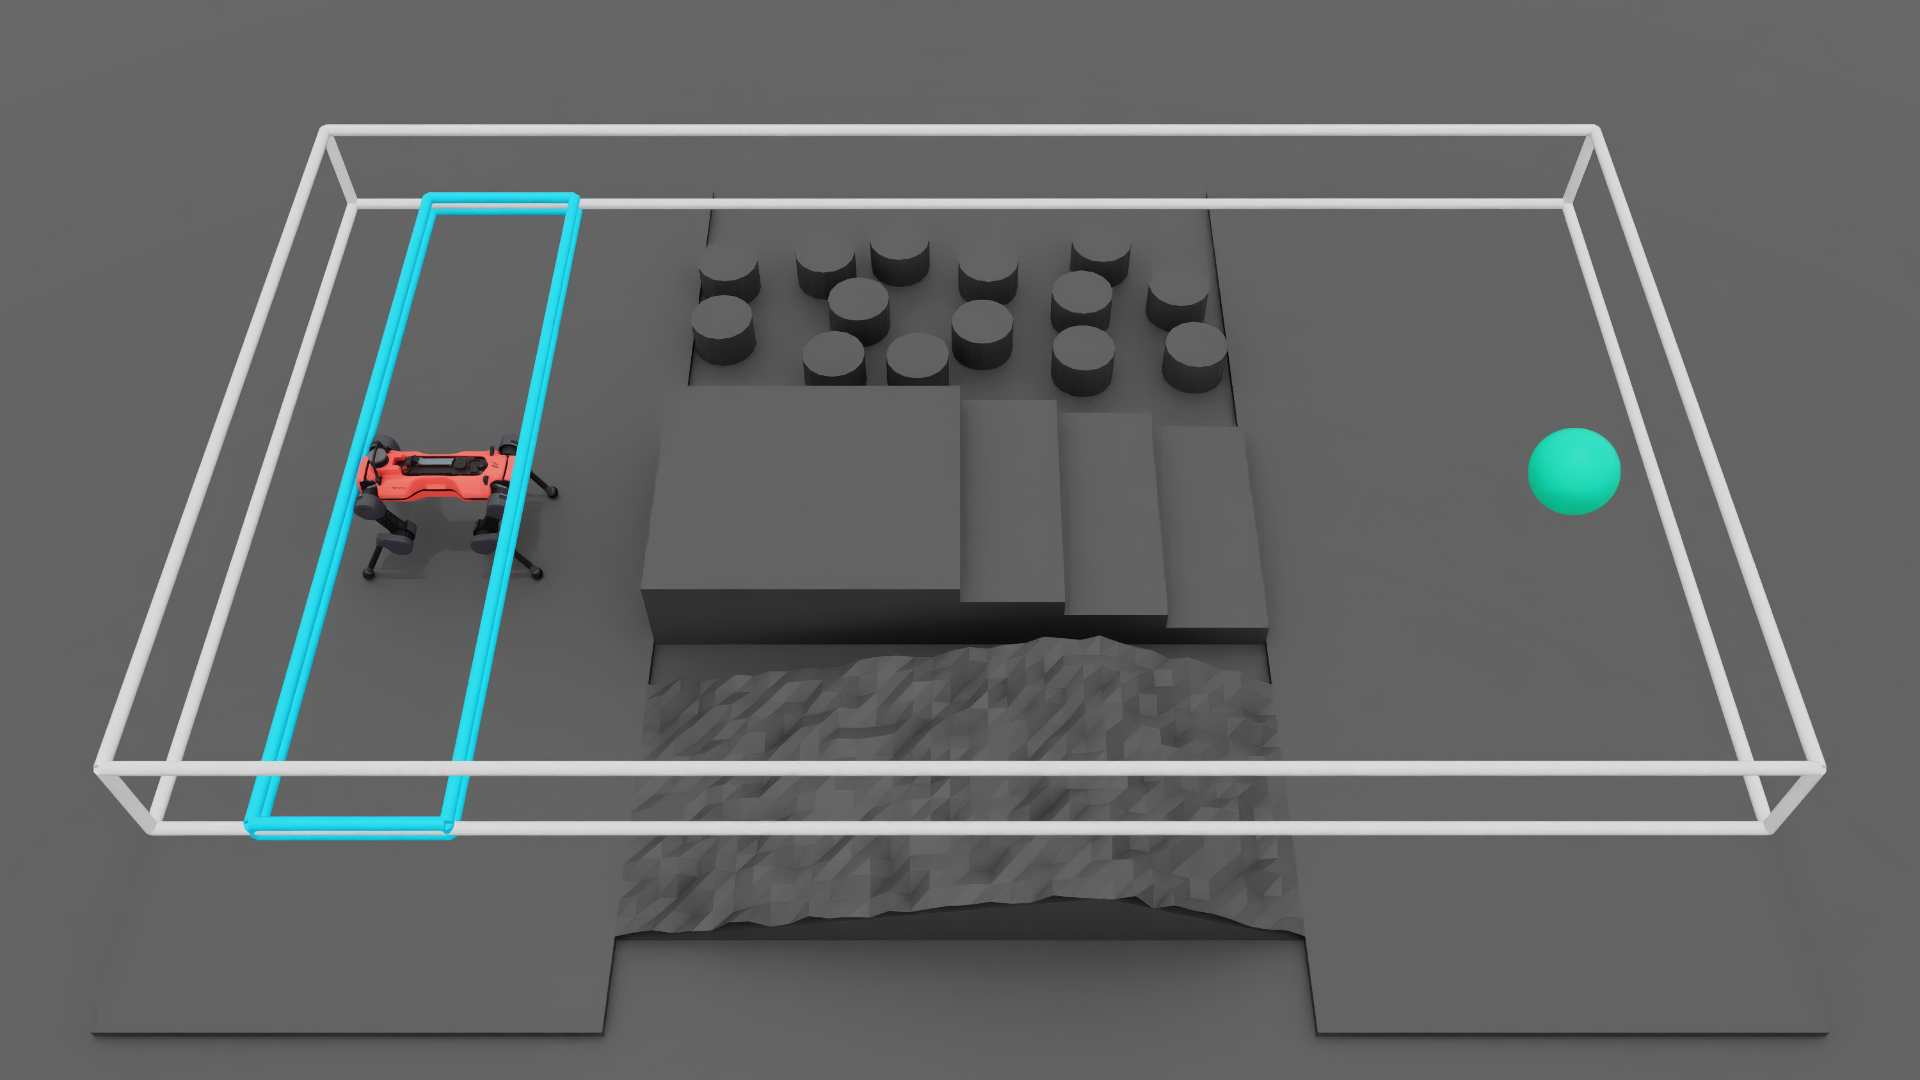
\includegraphics[width=\linewidth]{img/thumbnails/dtsg.png}
        \caption{Multiple terrain paths.}\label{fig:exp_renders_dtsg}
    \end{subfigure}
    \hfill
    \begin{subfigure}[t]{0.24\linewidth}
        \centering
        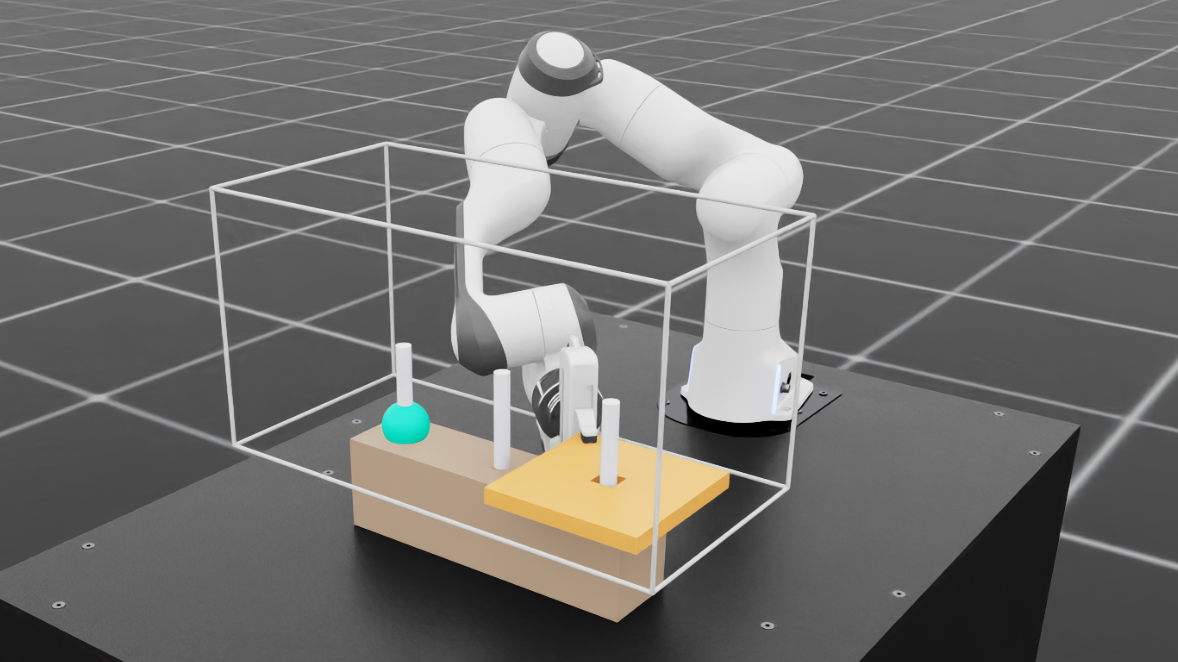
\includegraphics[width=\linewidth]{img/thumbnails/hanoi_p12.png}
        \caption{Tower of Hanoi.}\label{fig:exp_renders_hanoi_p12}
    \end{subfigure}
    \hfill\strut{}\\
    \hfill
    \begin{subfigure}[t]{0.24\linewidth}
        \centering
        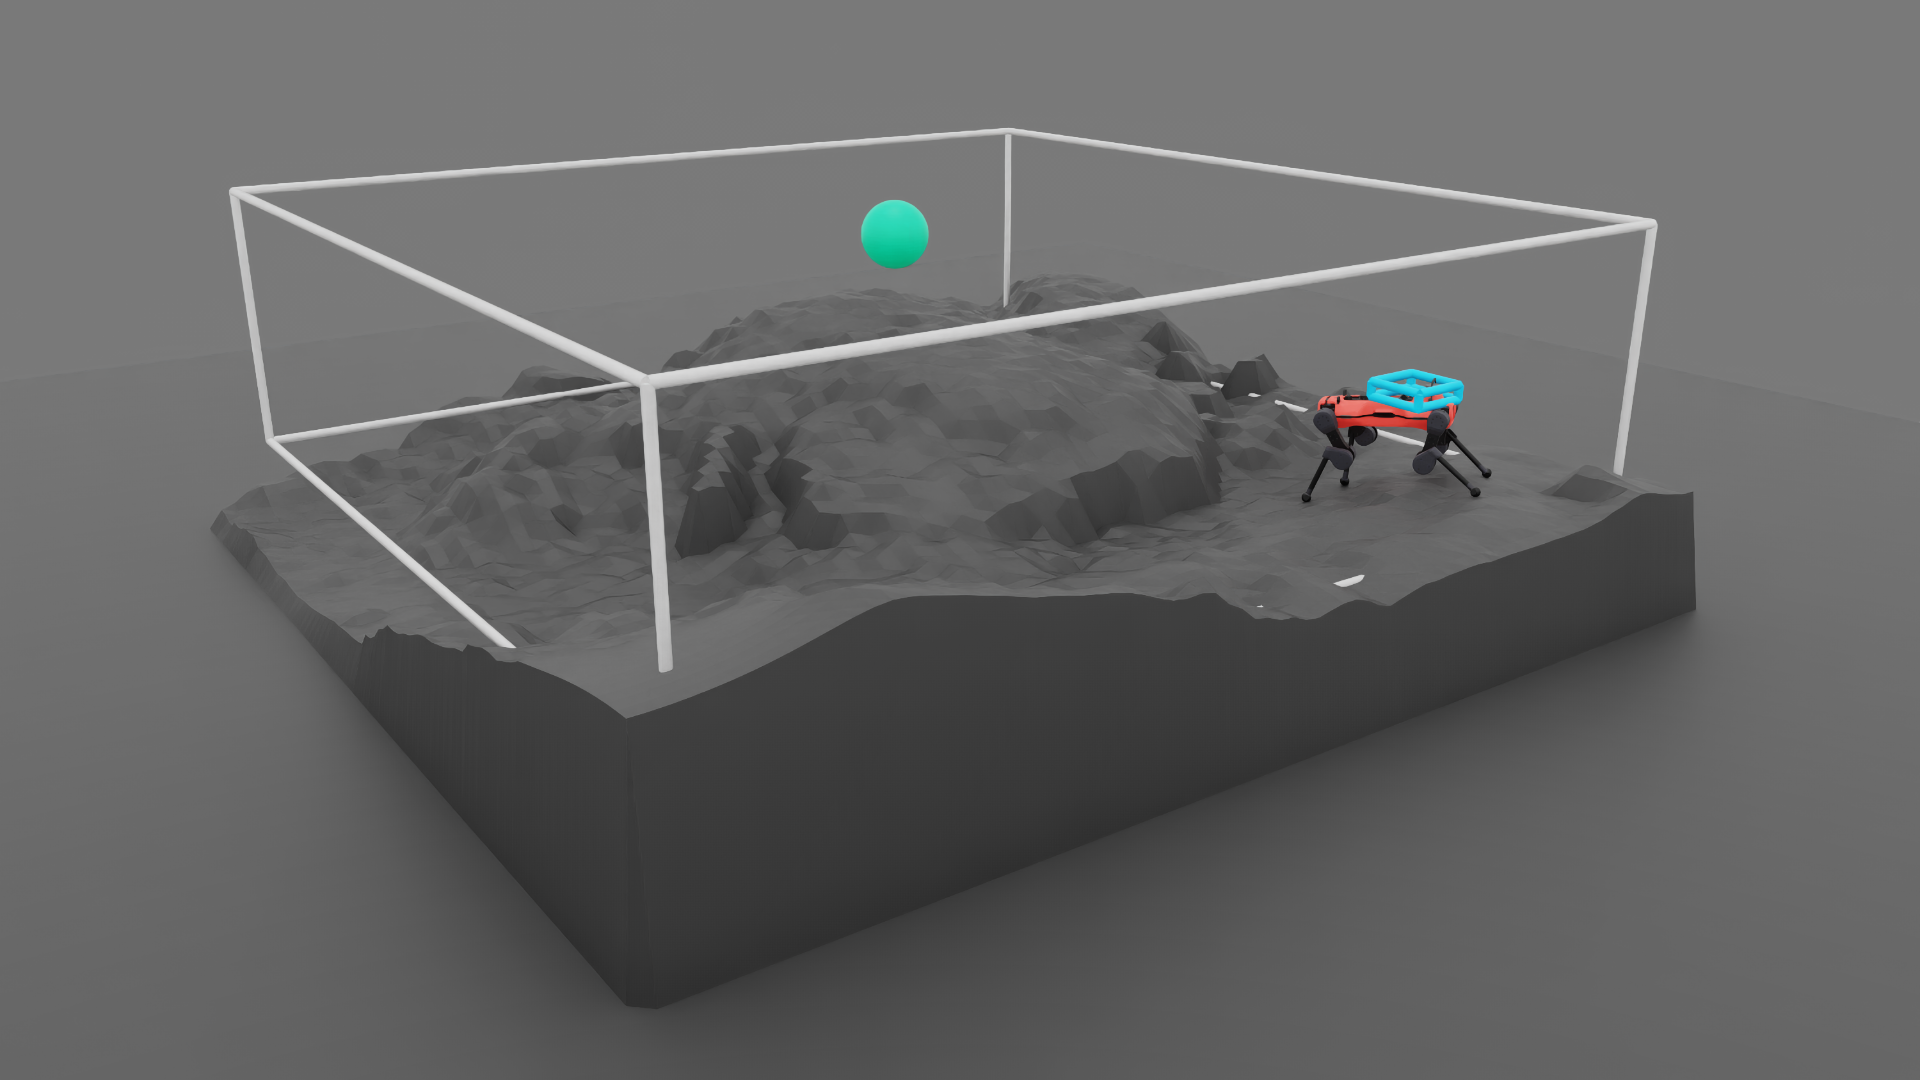
\includegraphics[width=\linewidth]{img/thumbnails/scan_boulder_small_rocks.png}
        \caption{Freestanding boulder I.}\label{fig:exp_renders_freestanding_boulder_I}
    \end{subfigure}
    \hfill
    \begin{subfigure}[t]{0.24\linewidth}
        \centering
        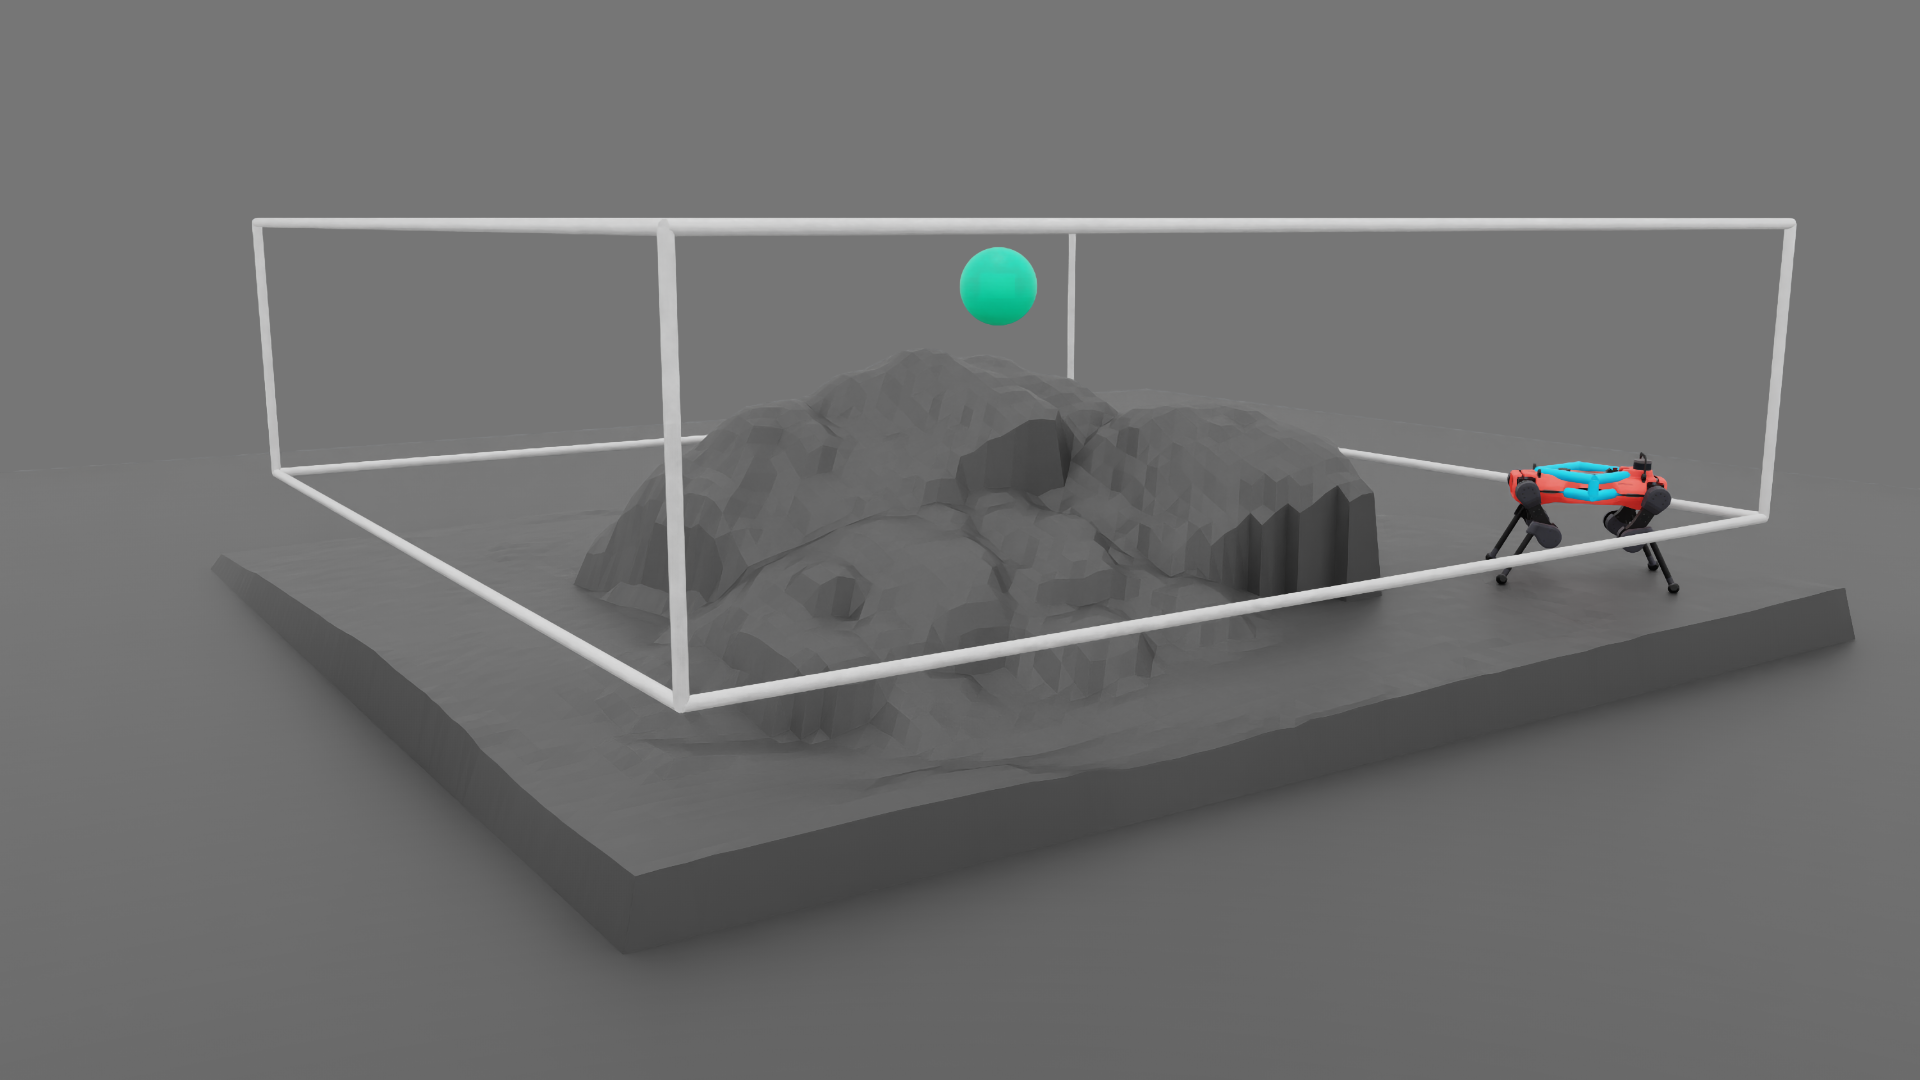
\includegraphics[width=\linewidth]{img/thumbnails/scan_freestanding_boulder.png}
        \caption{Freestanding boulder II.}\label{fig:exp_renders_freestanding_boulder_II}
    \end{subfigure}
    \hfill
    \begin{subfigure}[t]{0.24\linewidth}
        \centering
        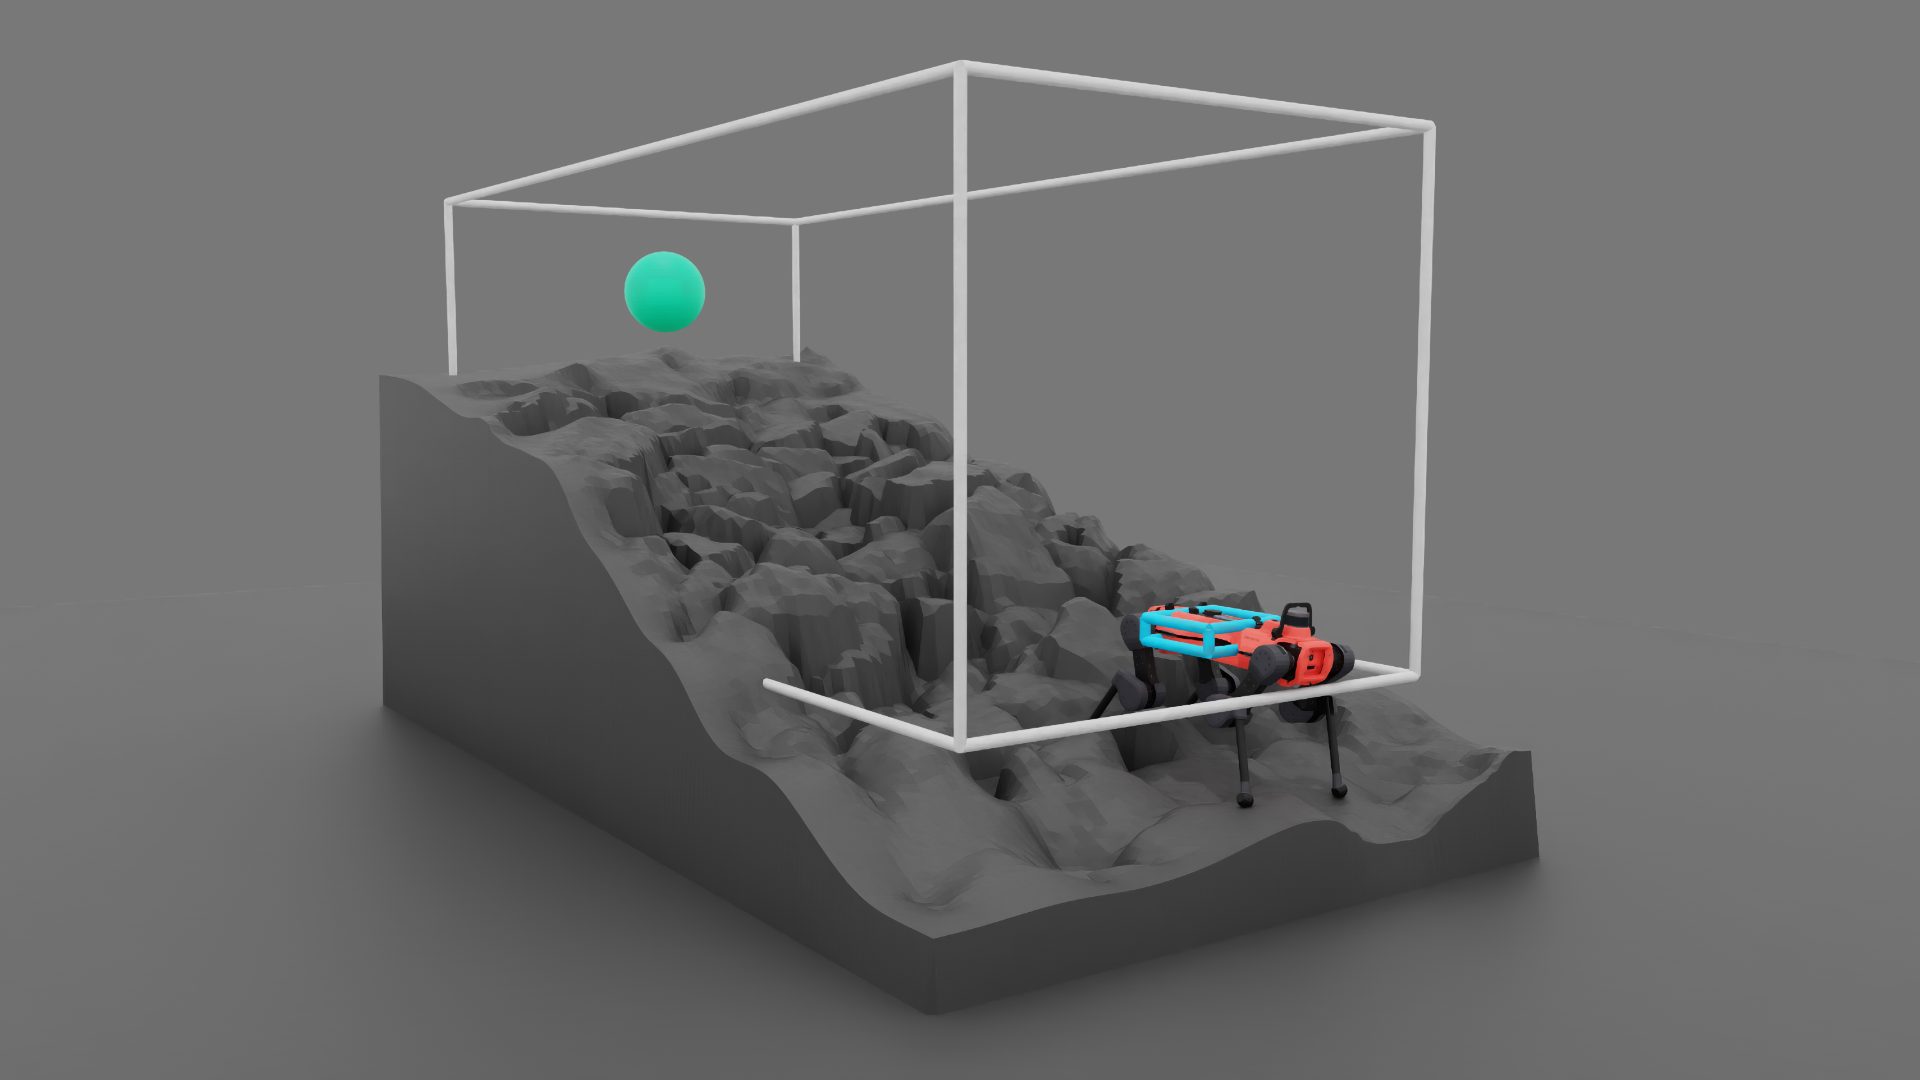
\includegraphics[width=\linewidth]{img/thumbnails/scan_rocky_ascent.png}
        \caption{Rocky ascent.}\label{fig:exp_renders_rocky_ascent}
    \end{subfigure}
    \hfill
    \begin{subfigure}[t]{0.24\linewidth}
        \centering
        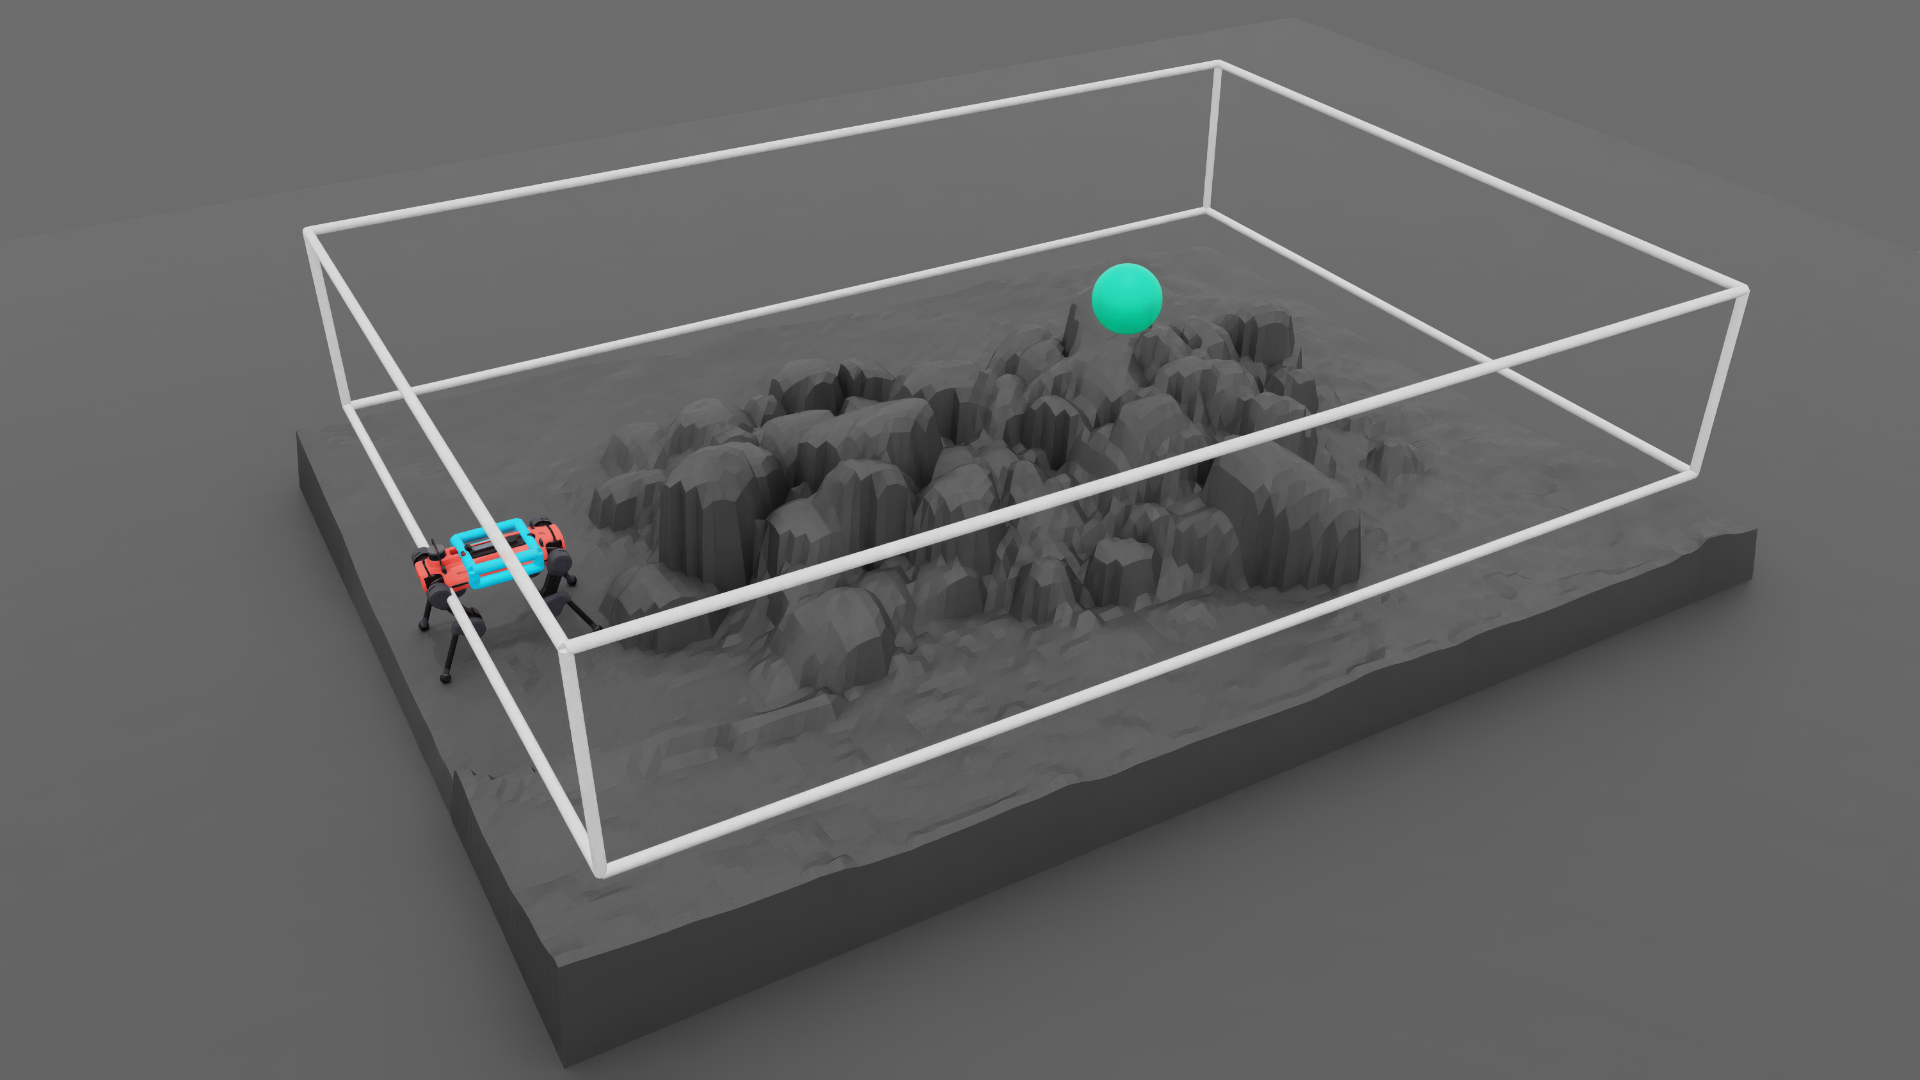
\includegraphics[width=\linewidth]{img/thumbnails/scan_small_rocks.png}
        \caption{Small stone field.}\label{fig:exp_renders_small_rocks}
    \end{subfigure}
    \hfill
    \caption{Experimental setup. {\color{cyan}Cyan} indicates the initial distribution, {\color{teal} green} the target goal, and the white box represents the task space.}\label{fig:experiment_renders}
\end{figure}

In all experiments, the rewards are defined as a combination of the sparse goal reward from Section~\ref{sec:problem_formulation} with $\epsilon = 0.25\,\mathrm{m}$, i.e., the agent has to reach the goal within a certain distance, and a termination penalty for collisions of the base with the terrain.

In the \textit{multiple terrain paths} experiments, a potential-based reward shaping term~\citep{ng1999policy}, which leaves the set of optimal policies of the underlying GA-MDP unchanged, is added to provide a reward signal strong enough for the no-curriculum PPO baseline to find solutions:
\begin{equation*}
    r_{\mathrm{progress}}(s_t, s_{t+1}, g) = \lVert \phi(s_t) - g \rVert - \gamma \lVert \phi(s_{t+1}) - g \rVert
\end{equation*}

\subsection{Sample Efficiency and Robustness}\label{sec:exp_main}
To evaluate sample efficiency and robustness, we compare our method BVER against state-of-the-art curriculum learning methods on a sparse-reward box climbing task. The task is defined as a goal-conditioned locomotion task where the agent has to reach a target goal position on top of a box from an initial distribution of start positions in front of the box. The task is challenging due to the sparse reward signal and the long horizon required to reach the goal.
\paragraph{Sample Efficiency:}
The results in Figure~\ref{fig:bench} already show a clear distinction between the vanilla PPO baseline, the curricula and the imitation learning methods (marked with $\star$). The policies trained on the initial distributions and no curriculum (vanilla PPO) are unable to solve the task, while training with random starts achieves a success rate of more than 95\%. This shows that the reward signal is attainable and the task solvable by initializing the agent closer to the goal.
Backplay~\citep{resnick2018backplay} shows the fastest convergence, and its advantage over RSI~\citep{peng2018deepmimic} shows the importance of ordering the task over training time. For the reference-free curricula, our method BVER shows the fastest convergence and highest success rate, outperforming both RC~\citep{florensa2017reverse} and random starts, while even surpassing RSI. BVER reaches a success rate of 95\% in roughly 65\% fewer training iterations than the best reference-free baseline.
% TODO: verify the 65% against the logged iteration counts (mean over seeds) and name the baseline.

\paragraph{Robustness:}
We evaluate the trained policies on (1) perturbations to the yaw angle used in the initialization, (2) variations in start positions (goal set to the target goal), and (3) variations in goal positions (initialized on the initial distribution). The results in Figure~\ref{fig:robustness} show that BVER's bidirectional curriculum leads to policies that can solve the task under various start-goal configurations, while the other curricula fail to generalize to unseen configurations.
\begin{figure}[h]
    \centering
    \hfill
    \begin{subfigure}[c]{0.6\linewidth}
        \centering
        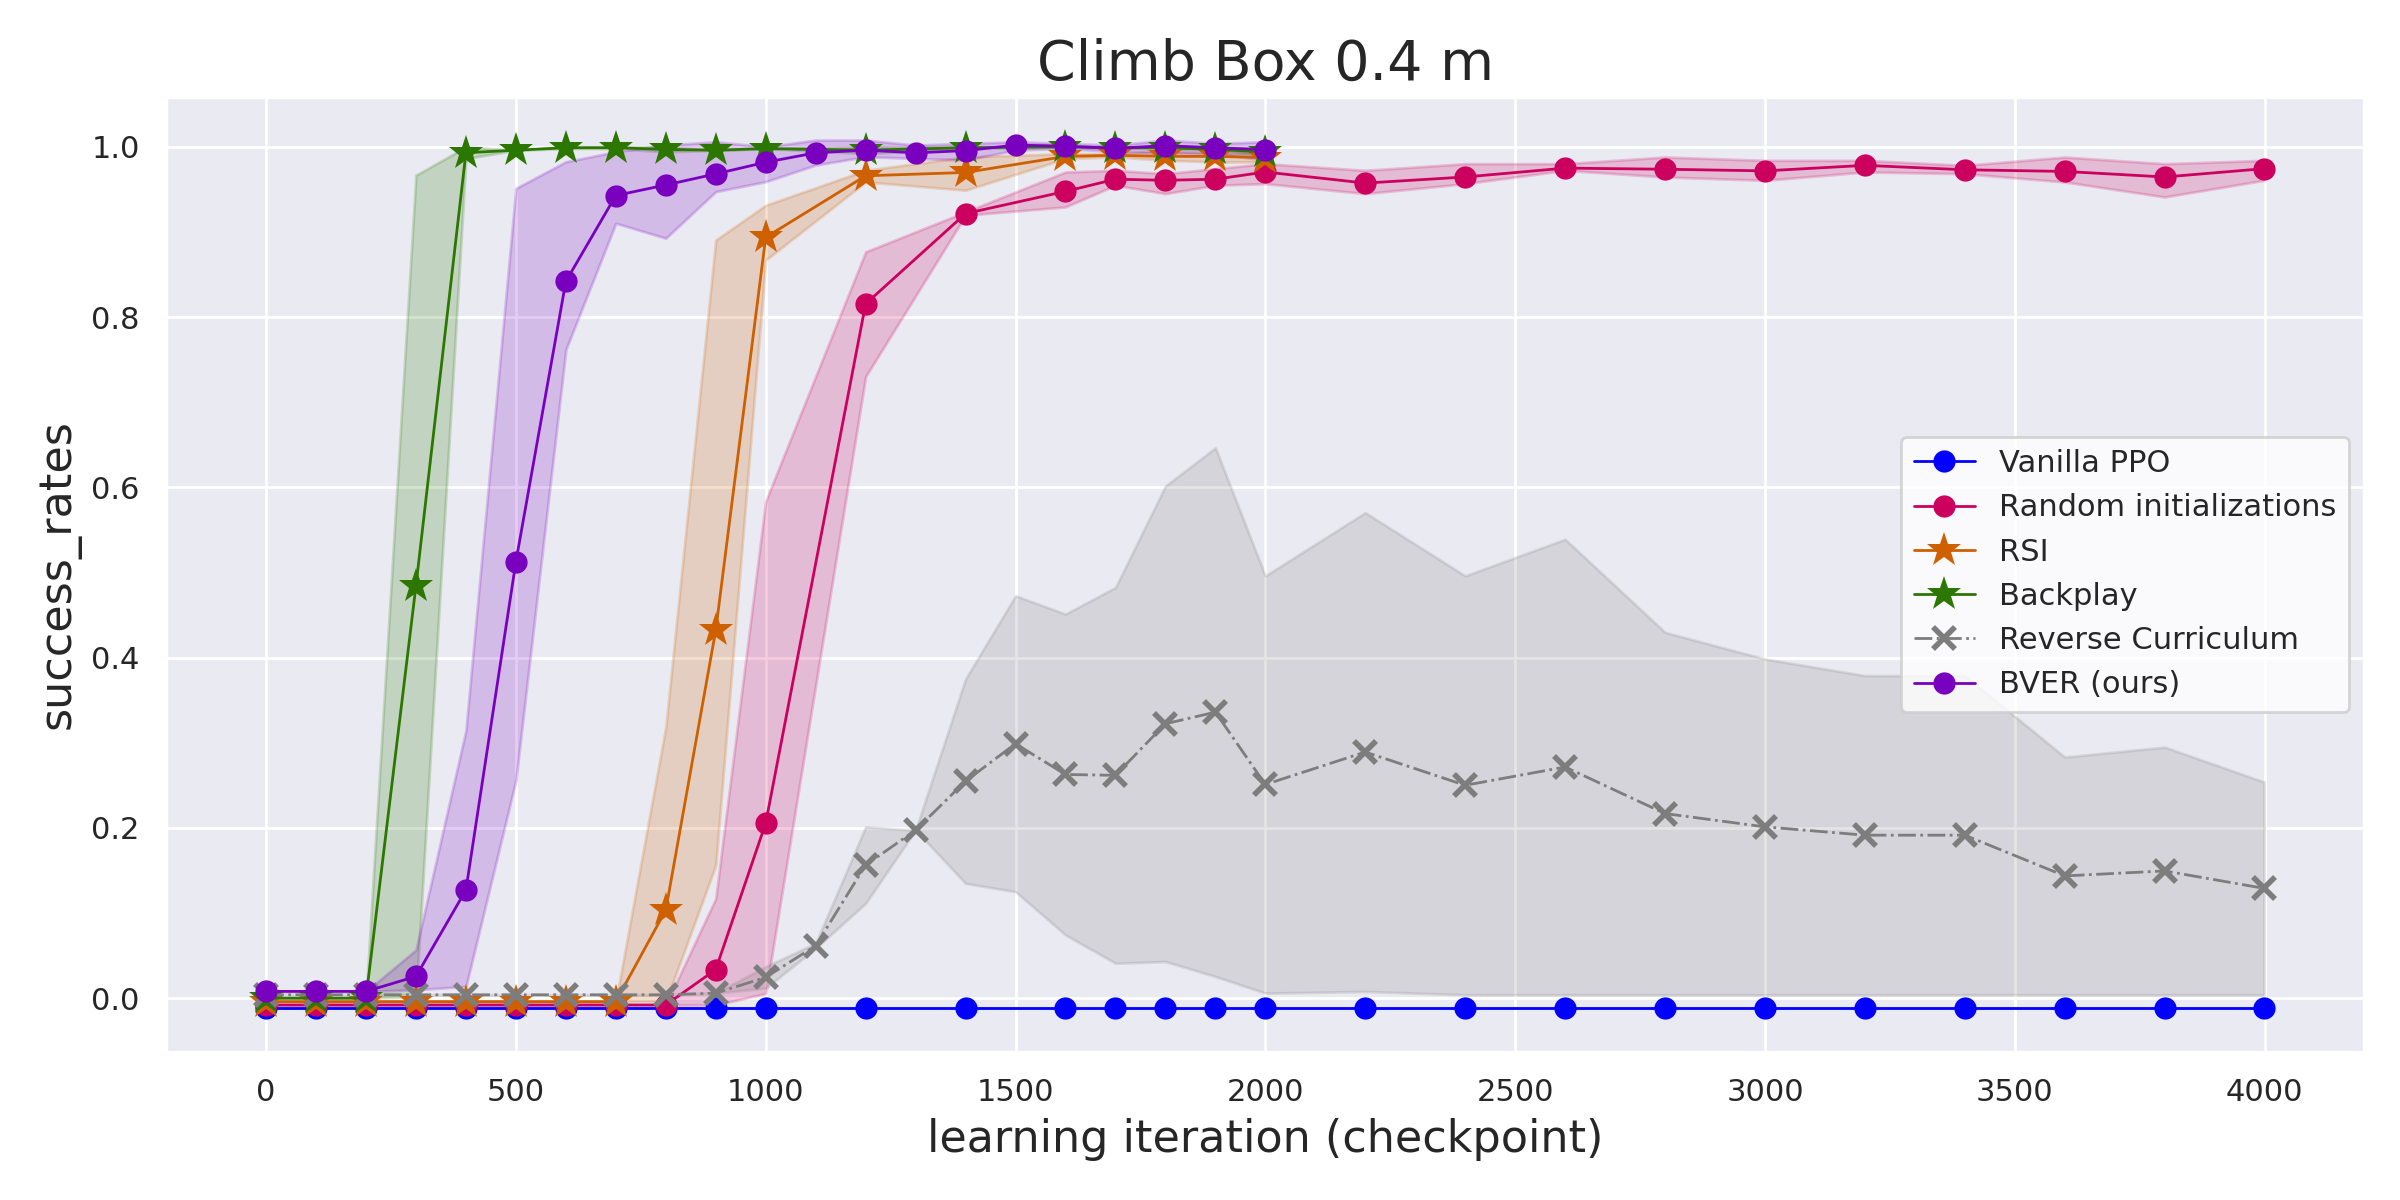
\includegraphics[width=\linewidth]{img/sb/eval_comparison_41_up_clean_comp.png}
        \caption{BVER is able to achieve a success rate of over 95\% faster than all other reference-free curricula and even faster than one reference-based method (RSI).}\label{fig:bench}
    \end{subfigure}
    \hfill
    \begin{subfigure}[c]{0.3\linewidth}
        \centering
        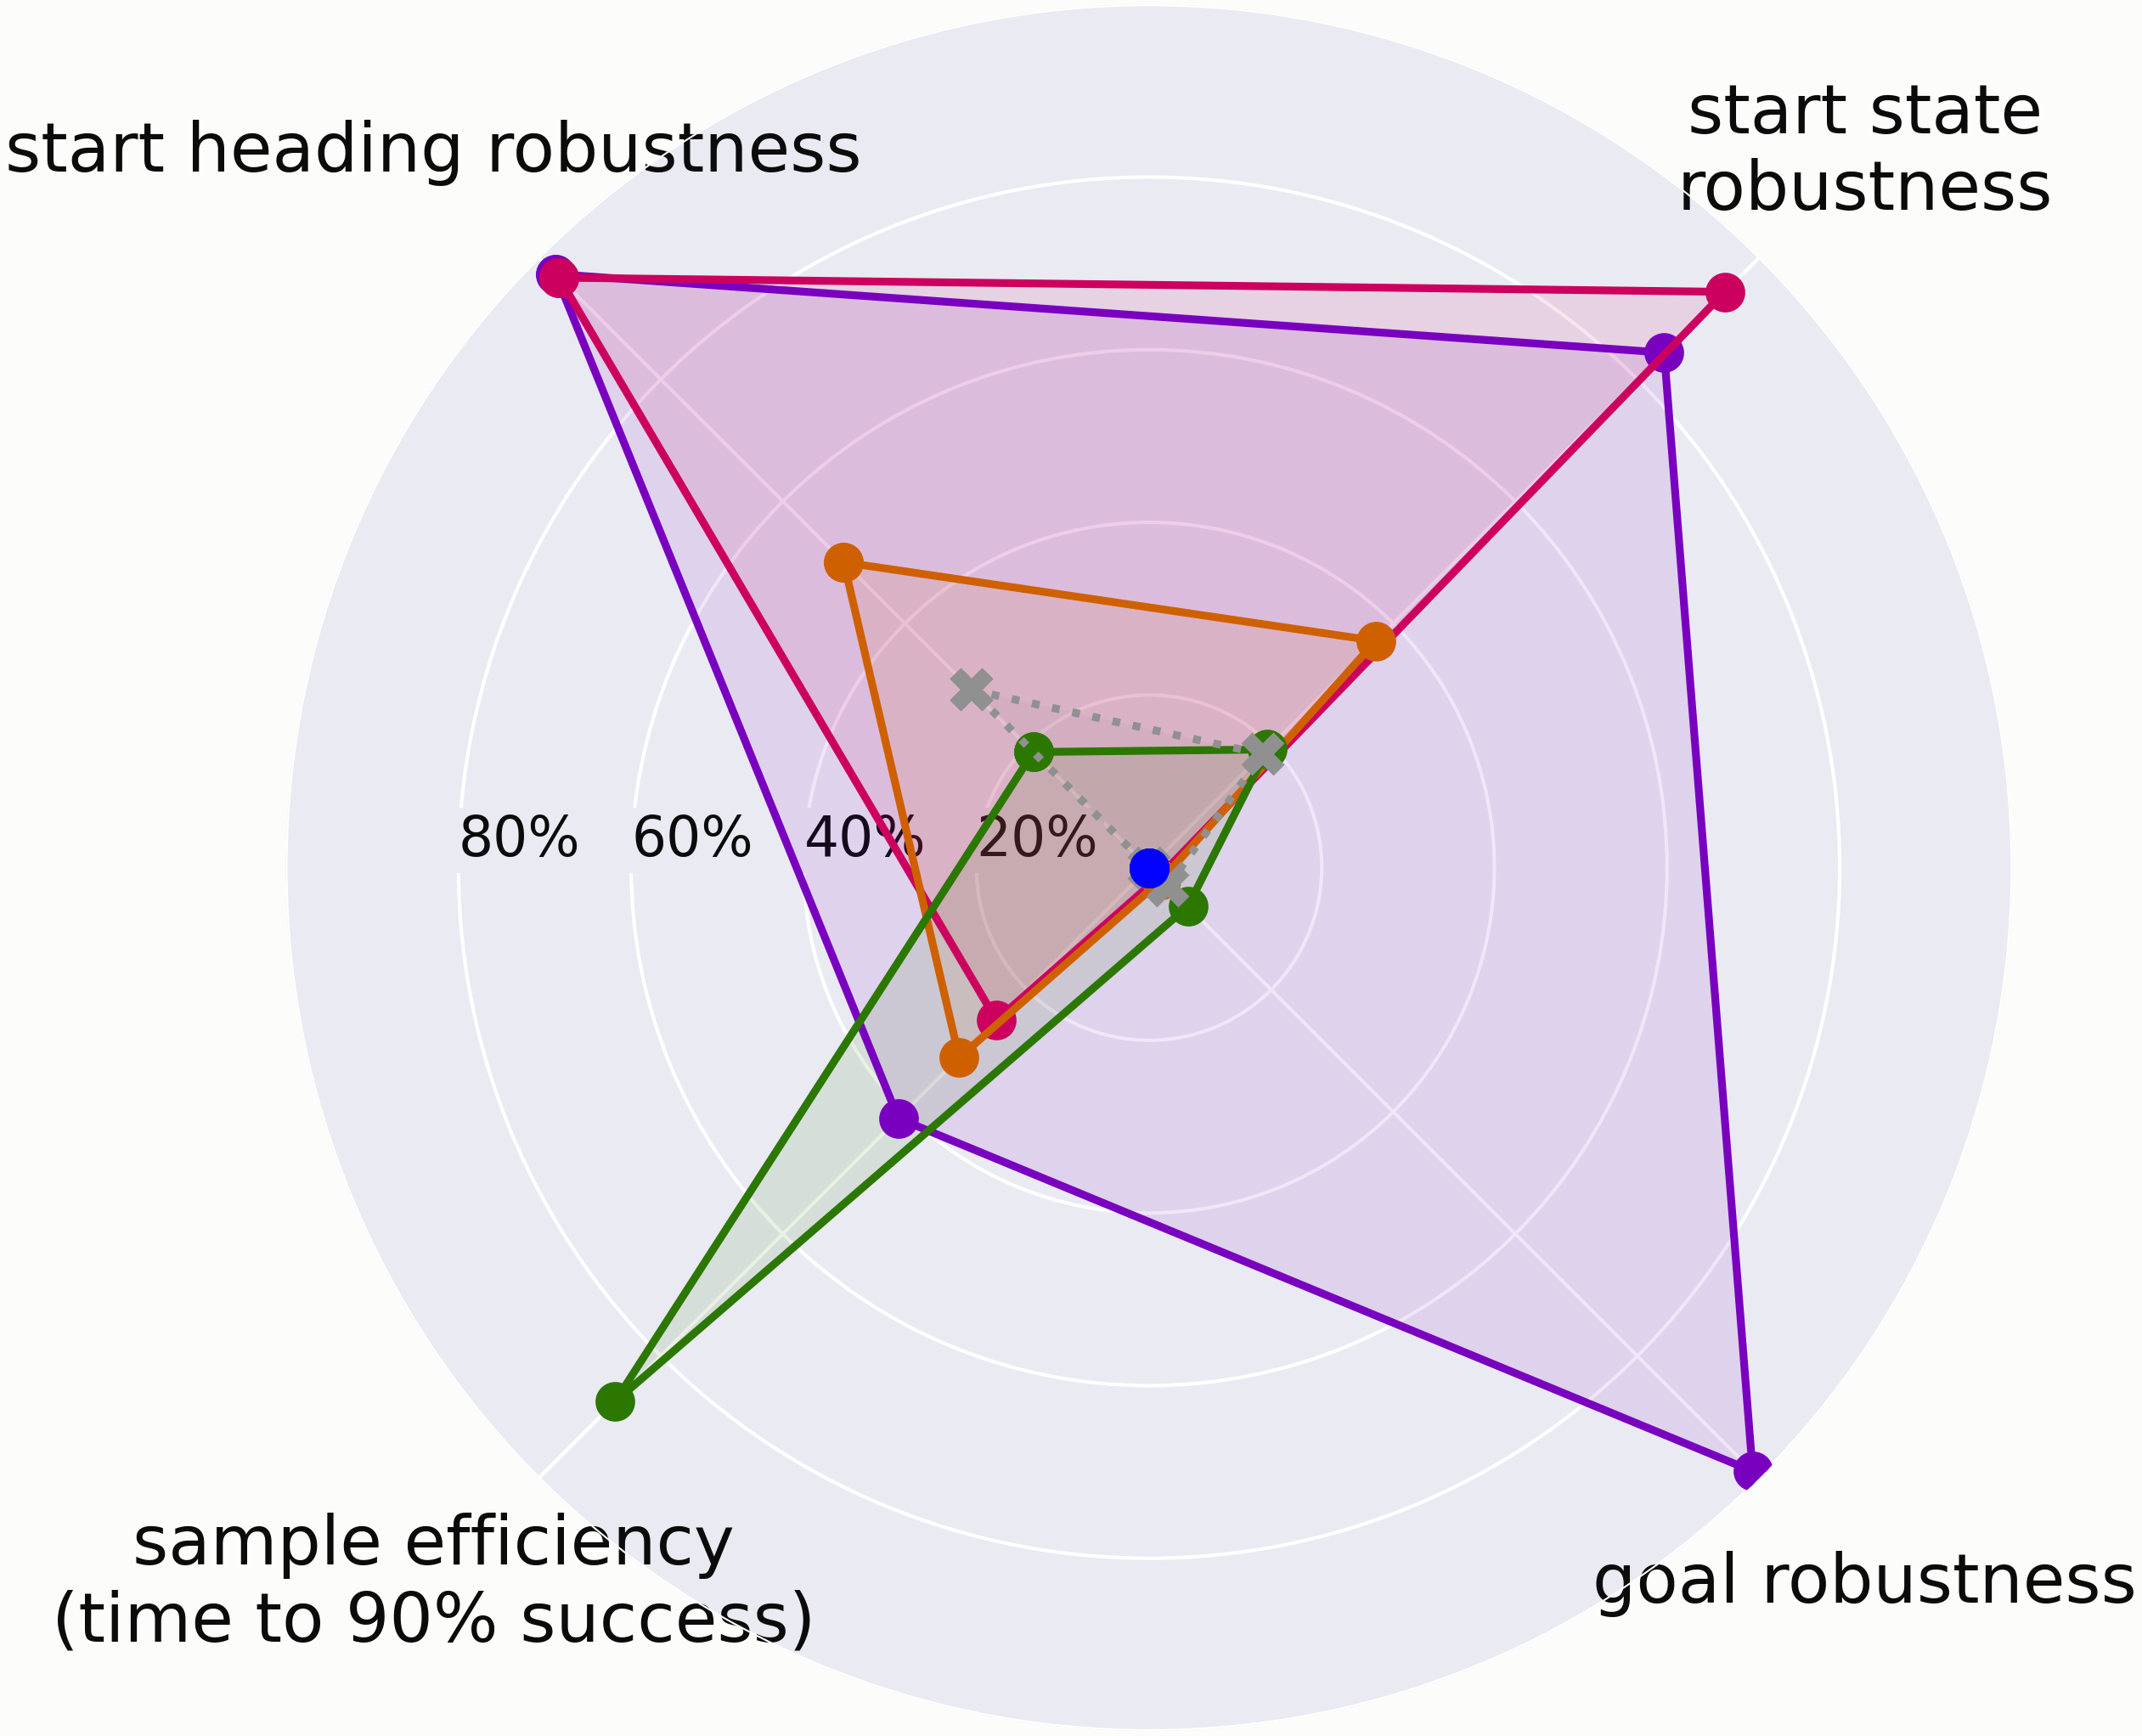
\includegraphics[width=\linewidth]{img/sb/robustness_spider_headline_nolegend.png}
        \caption{BVER's start-goal curriculum leads to policies that can solve the task under various start-goal configurations.}\label{fig:robustness}
    \end{subfigure}
    \hfill\strut{}
    \caption{Sample efficiency and robustness evaluated on a sparse-reward box climbing task.}\label{fig:eval_04}
\end{figure}

\subsection{Ablations: Forwards / Backwards Symmetry}\label{sec:exp_ablations}

\paragraph{Maze ablations:}\label{sec:exp_ablations_maze}
To evaluate the contribution of individual components of BVER, we conduct further ablation studies on three maze environments (Figure~\ref{fig:maze_layout}) similar to those used in prior work~\citep{florensa2017reverse,cho2023outcome}. Specifically, the agent ({\color{orange}orange point mass}) has to find a path from the initial distribution ({\color{cyan}cyan rectangle}) to the goal ({\color{teal}green ball}). First, we evaluate the effect of our curriculum against a baseline that does not use any curriculum (\textit{vanilla PPO}) and a simple curriculum that samples intermediate goals (to reach from the start) and intermediate starts (from which to reach the target goal) randomly from the free space (\textit{random initializations}). The results in Figure~\ref{fig:maze_ablation_bench} show that both curricula enable finding solutions in all three environments, whereas vanilla PPO does not. In the more complex \textit{N-maze} and \textit{large-maze} environments, BVER shows faster convergence than the random curriculum.

We compare using only the forwards expansion, only the backwards expansion, and the bidirectional expansion in Figure~\ref{fig:maze_ablation_dir}. In addition, we evaluate the effect of connecting the two frontiers by comparing a version of BVER that only samples from the task space to a version that samples from both the task space and the other frontier. The results in Figure~\ref{fig:maze_ablation_connect} show that connecting the two frontiers leads to better sample efficiency in the cases where the optimal path covers only a small fraction of the total search space (\textit{N-maze} and \textit{large-maze}). However, there is no significant difference between connect ratios above 0.5.
\begin{figure}[h]
    \centering
    \hfill
    \begin{subfigure}[c]{0.11\linewidth}
        \centering
        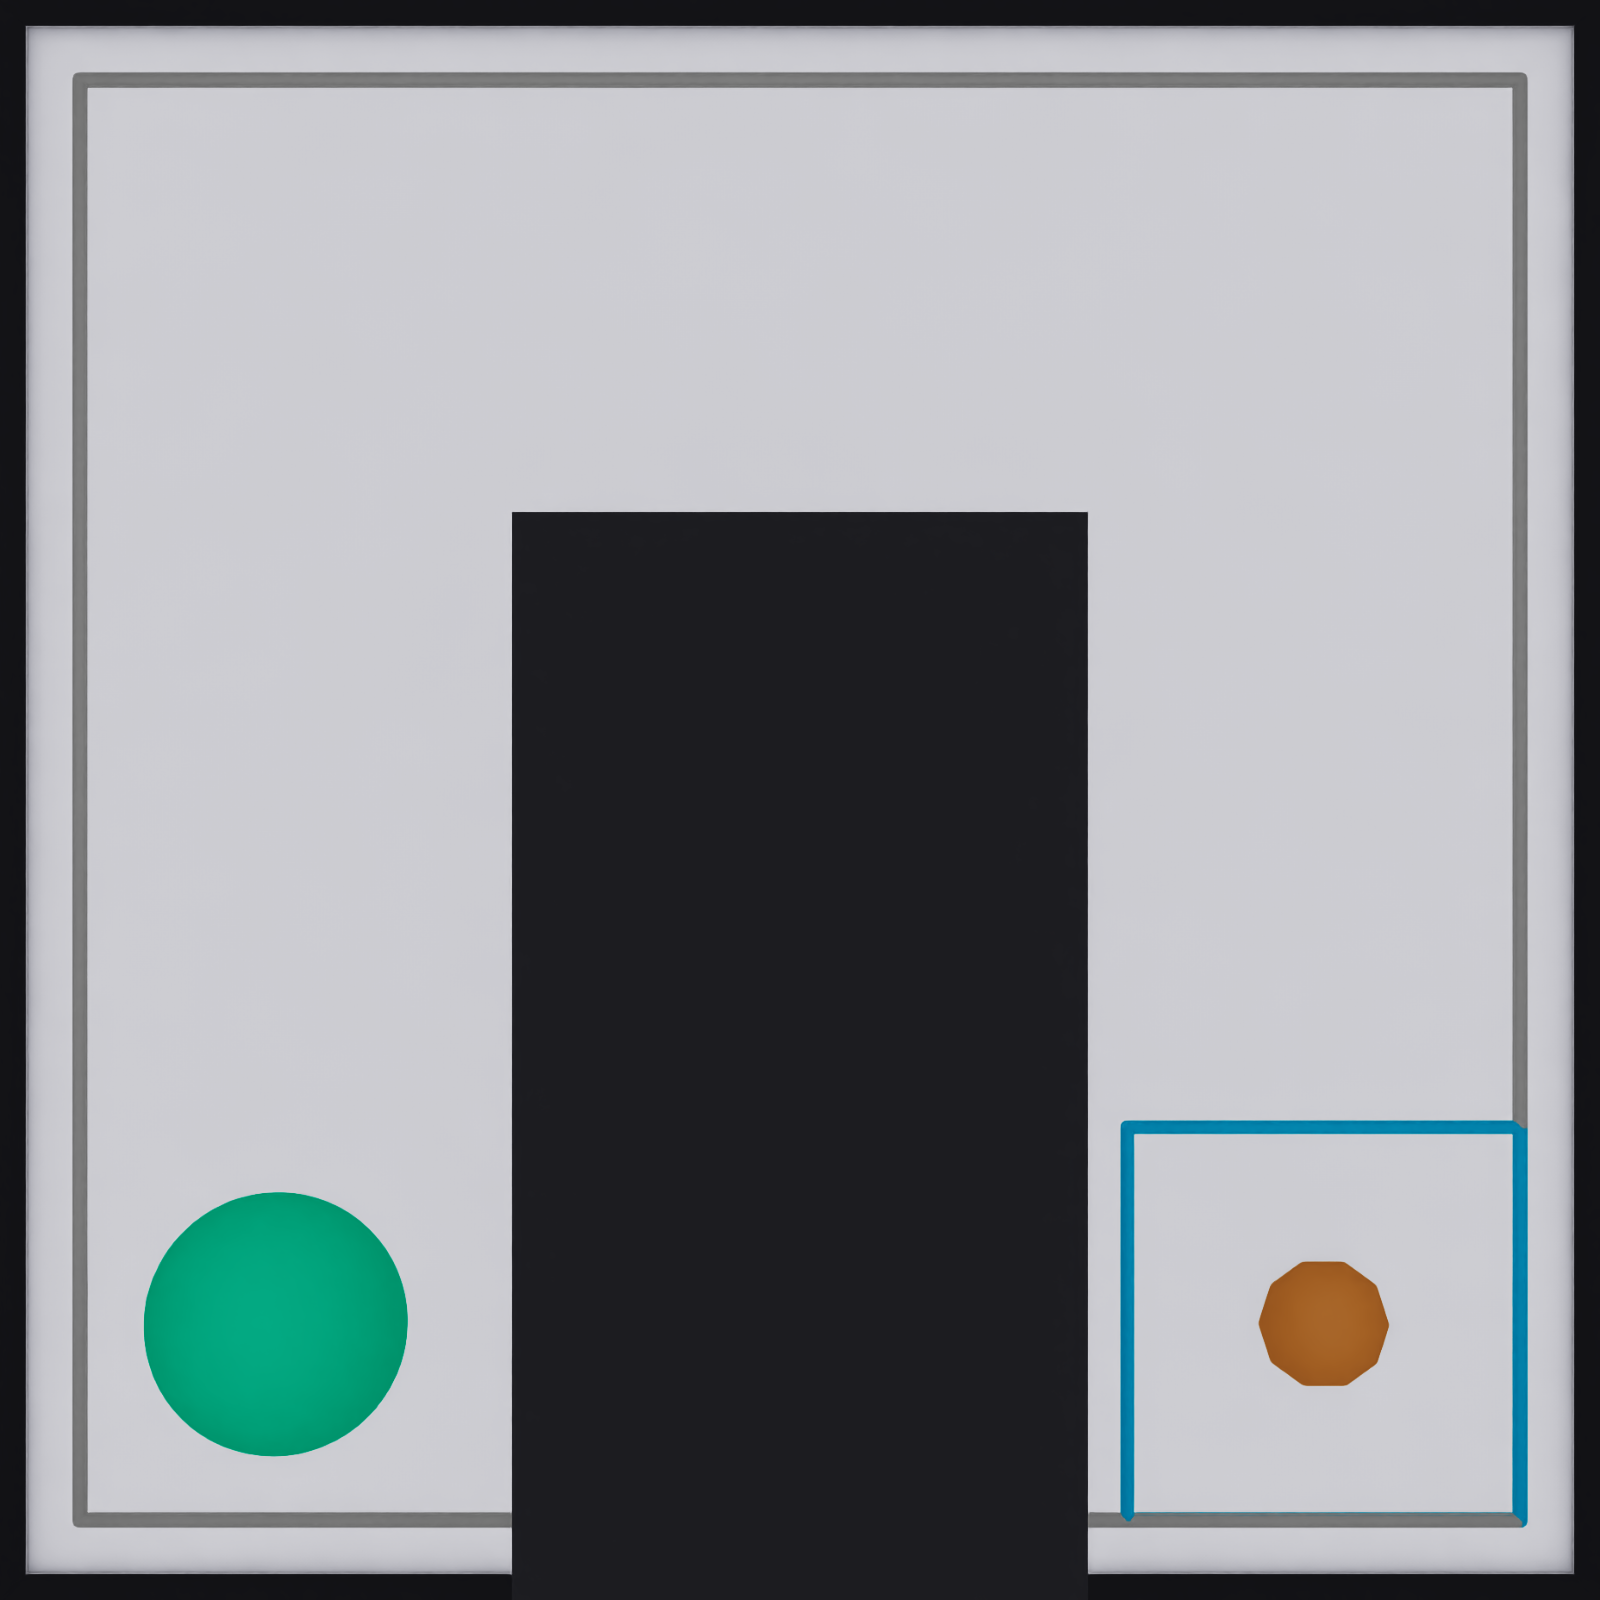
\includegraphics[width=\linewidth]{img/maze/layouts/maze_u.png}
    \end{subfigure}
    \hfill
    \begin{subfigure}[c]{0.29\linewidth}
        \centering
        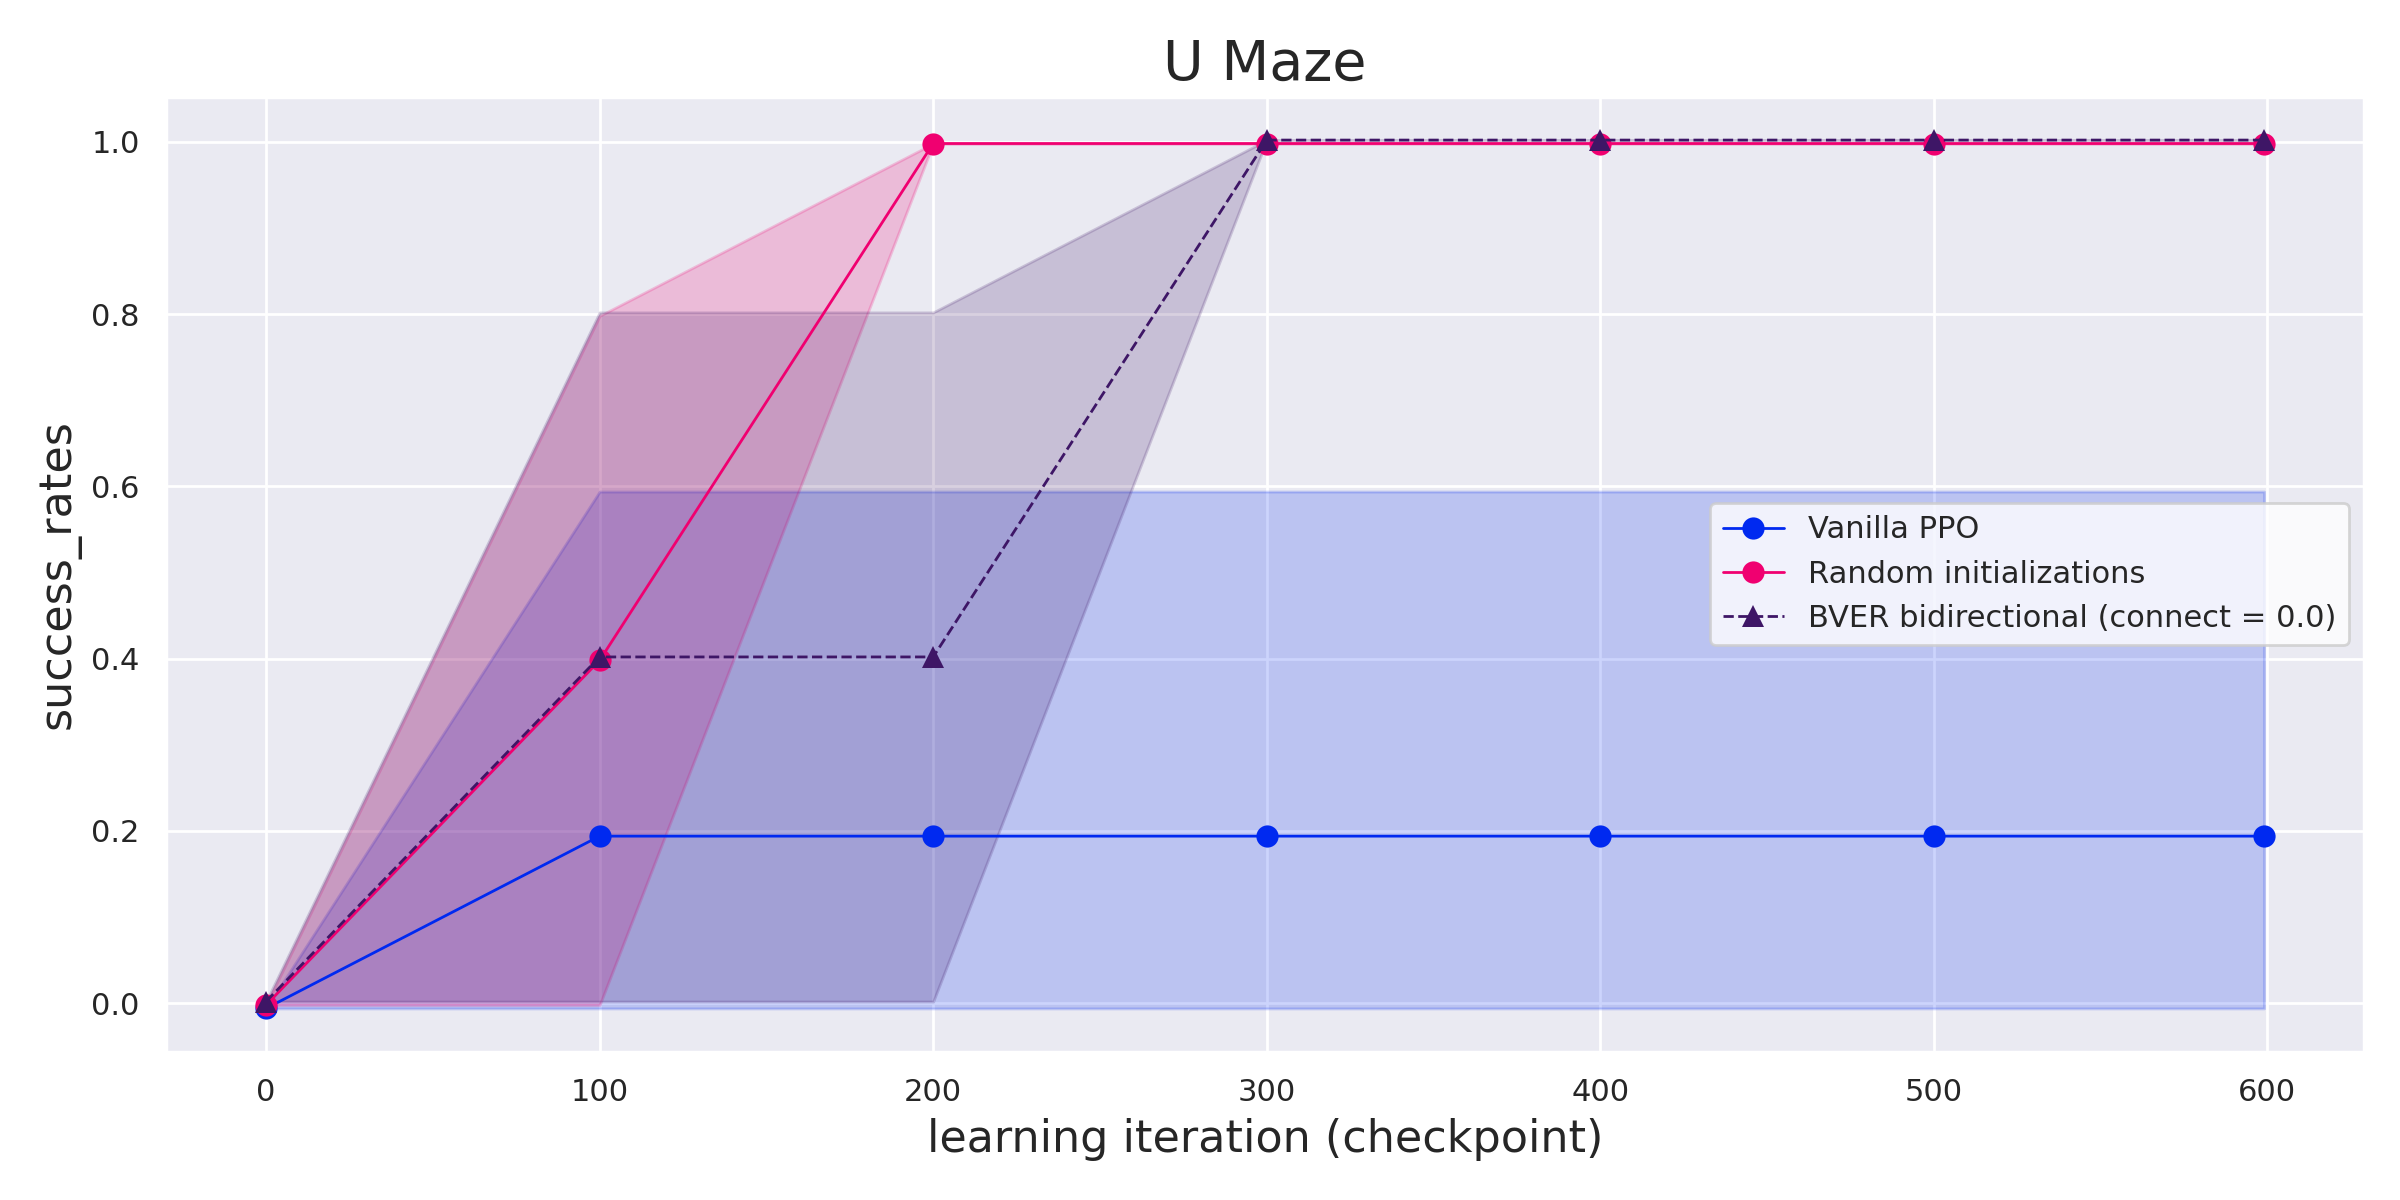
\includegraphics[width=\linewidth]{img/maze/u/eval_comparison_u_maze_bench.png}
    \end{subfigure}
    \hfill
    \begin{subfigure}[c]{0.29\linewidth}
        \centering
        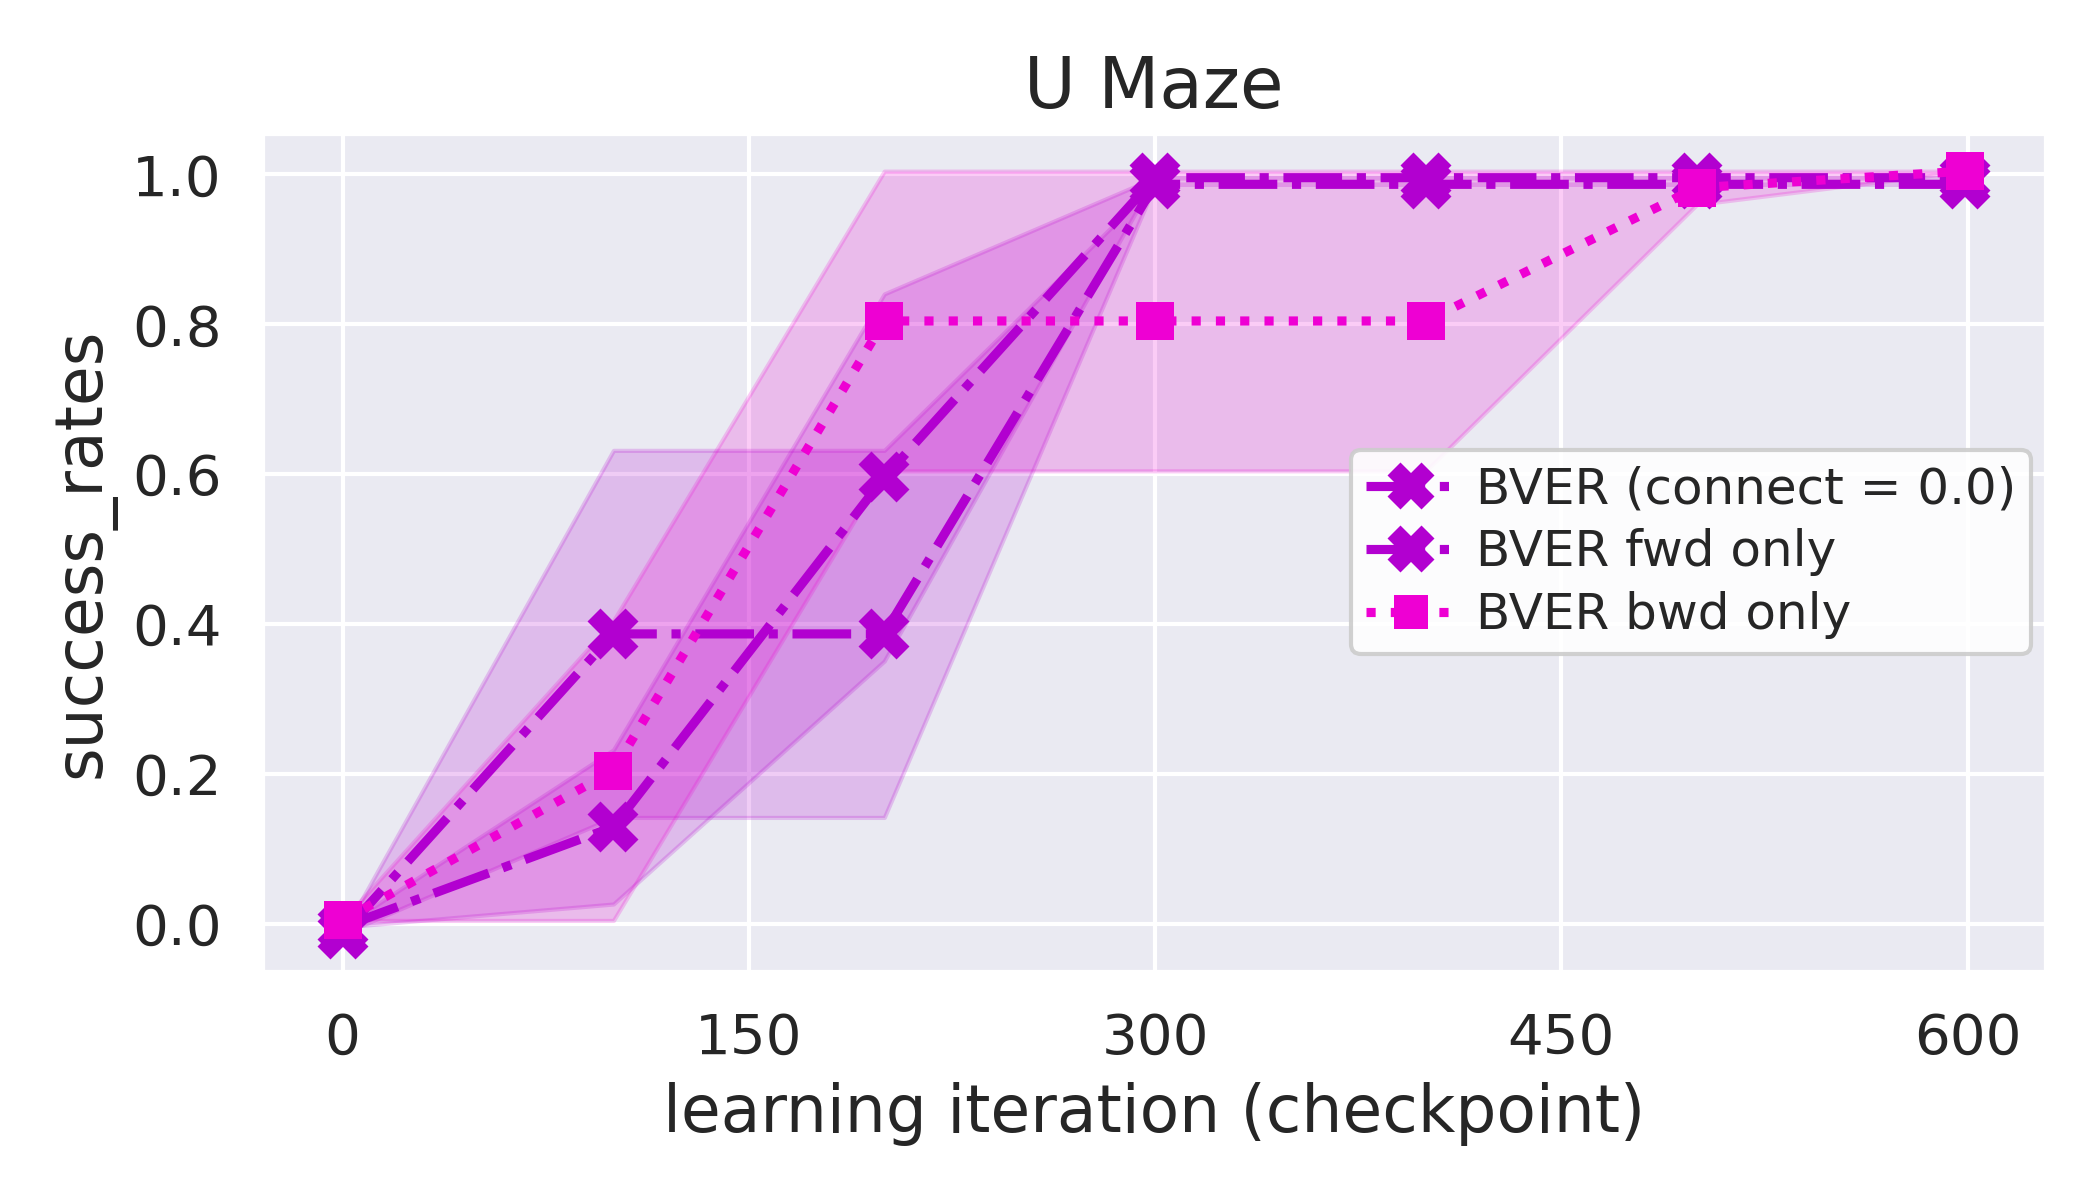
\includegraphics[width=\linewidth]{img/maze/u/eval_comparison_u_maze_abl_dir.png}
    \end{subfigure}
    \hfill
    \begin{subfigure}[c]{0.29\linewidth}
        \centering
        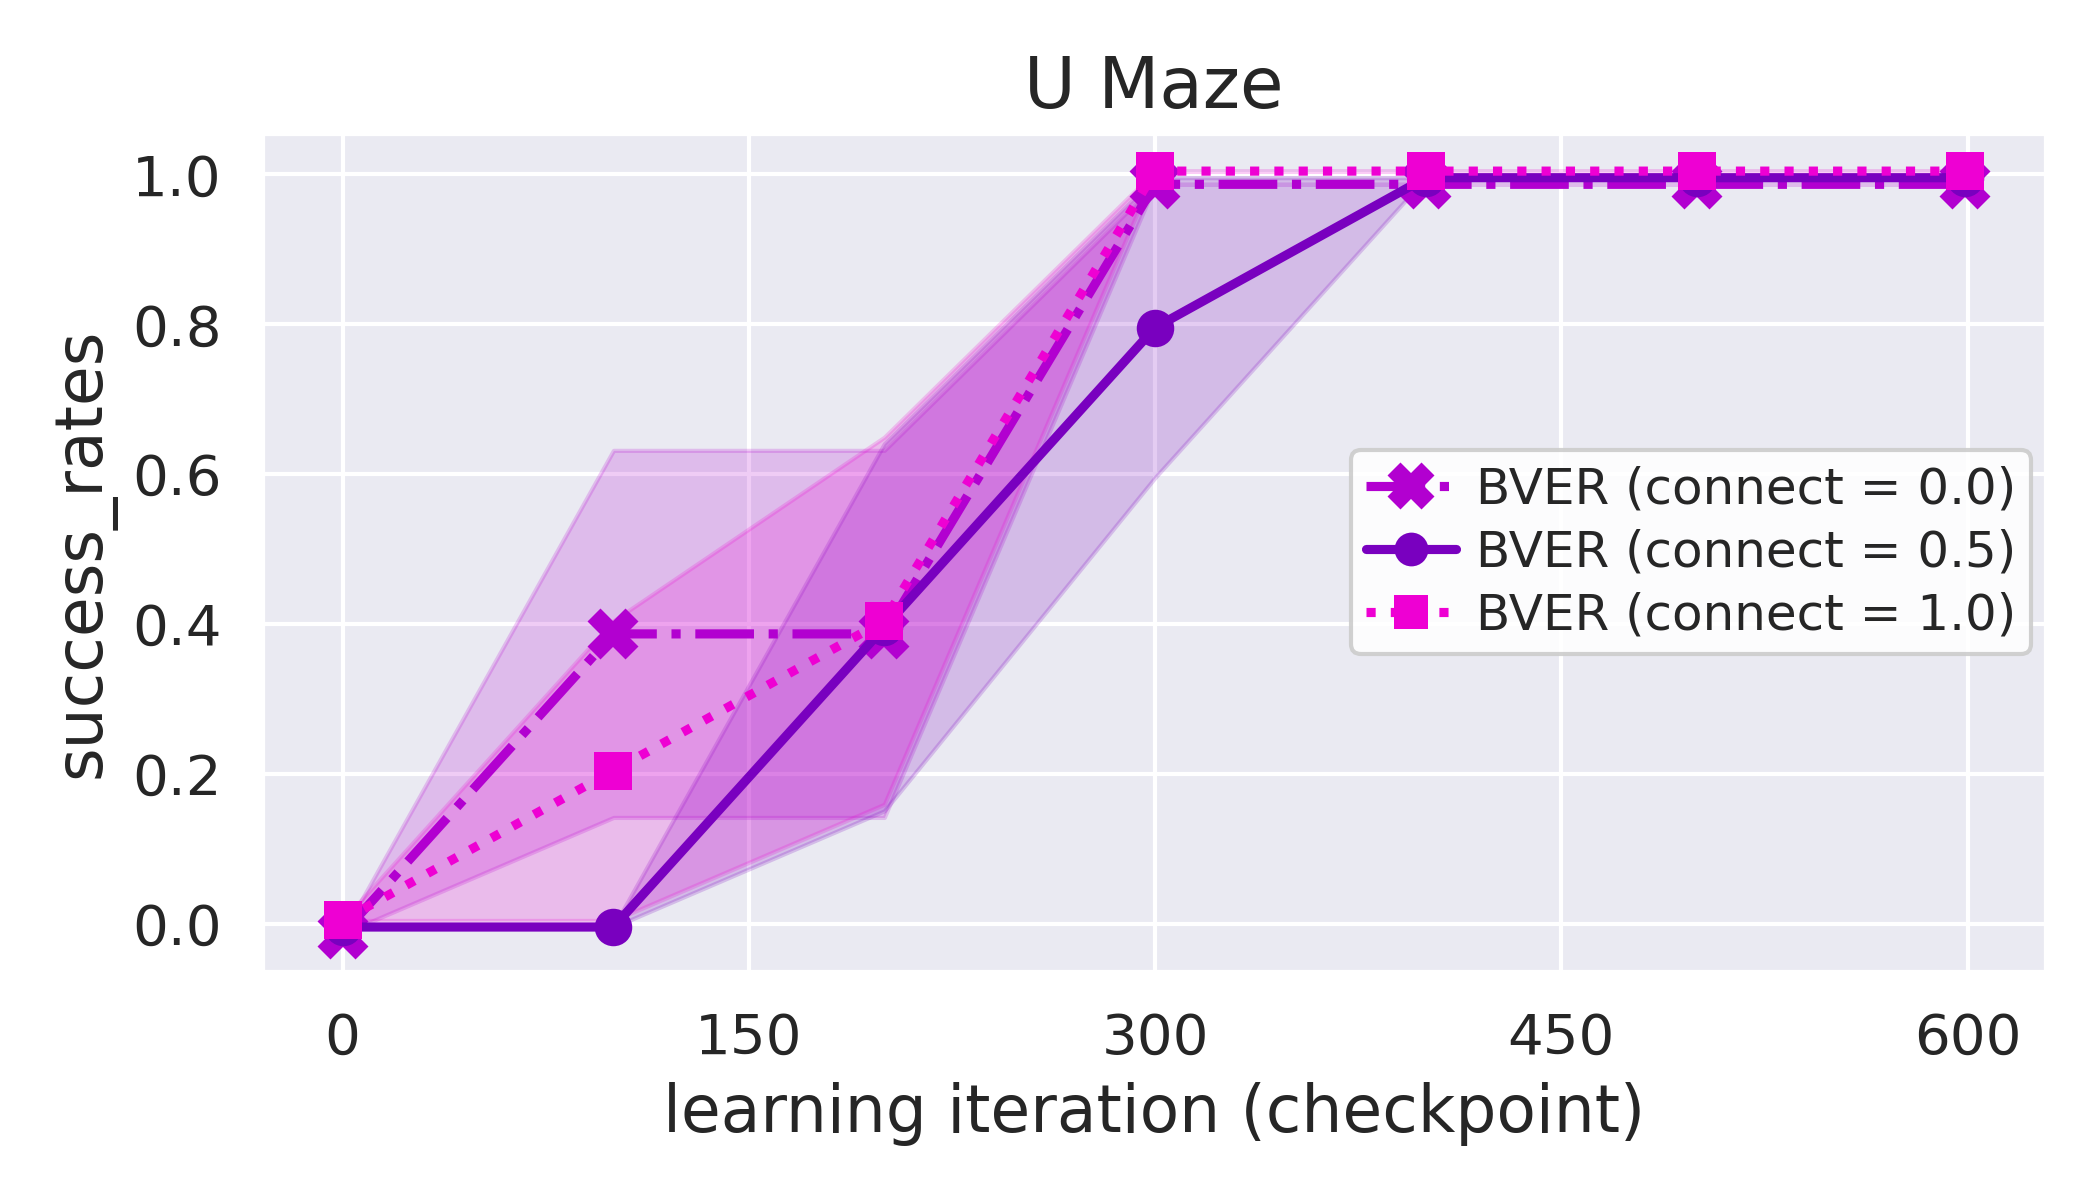
\includegraphics[width=\linewidth]{img/maze/u/eval_comparison_u_maze_abl_connect.png}
    \end{subfigure}
    %
    \hfill\strut{}\\[-2em]
    \hfill
    \begin{subfigure}[c]{0.11\linewidth}
        \centering
        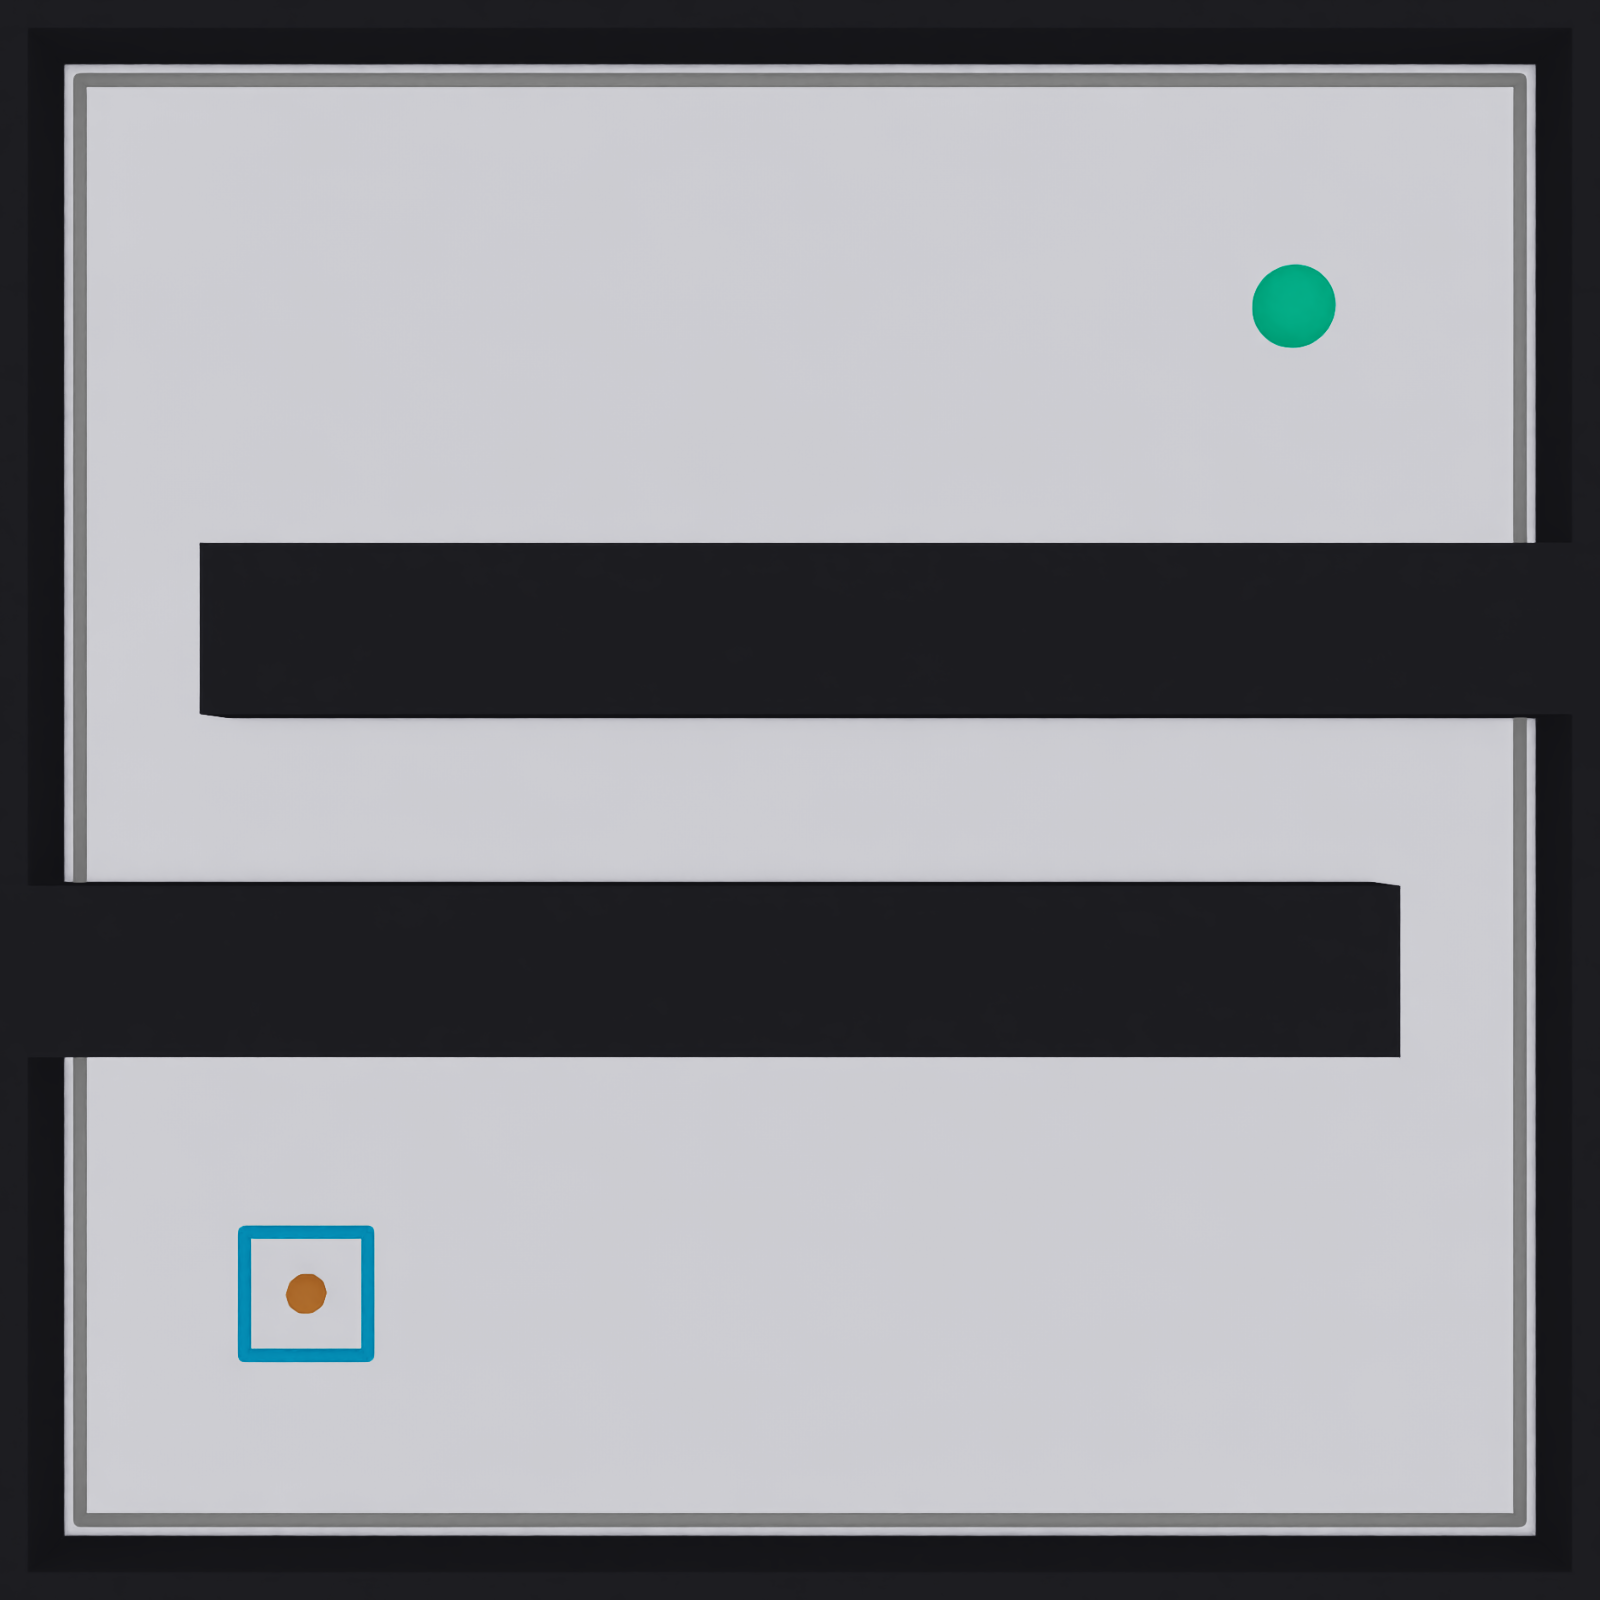
\includegraphics[width=\linewidth]{img/maze/layouts/maze_serpentine.png}
    \end{subfigure}
    \hfill
    \begin{subfigure}[c]{0.29\linewidth}
        \centering
        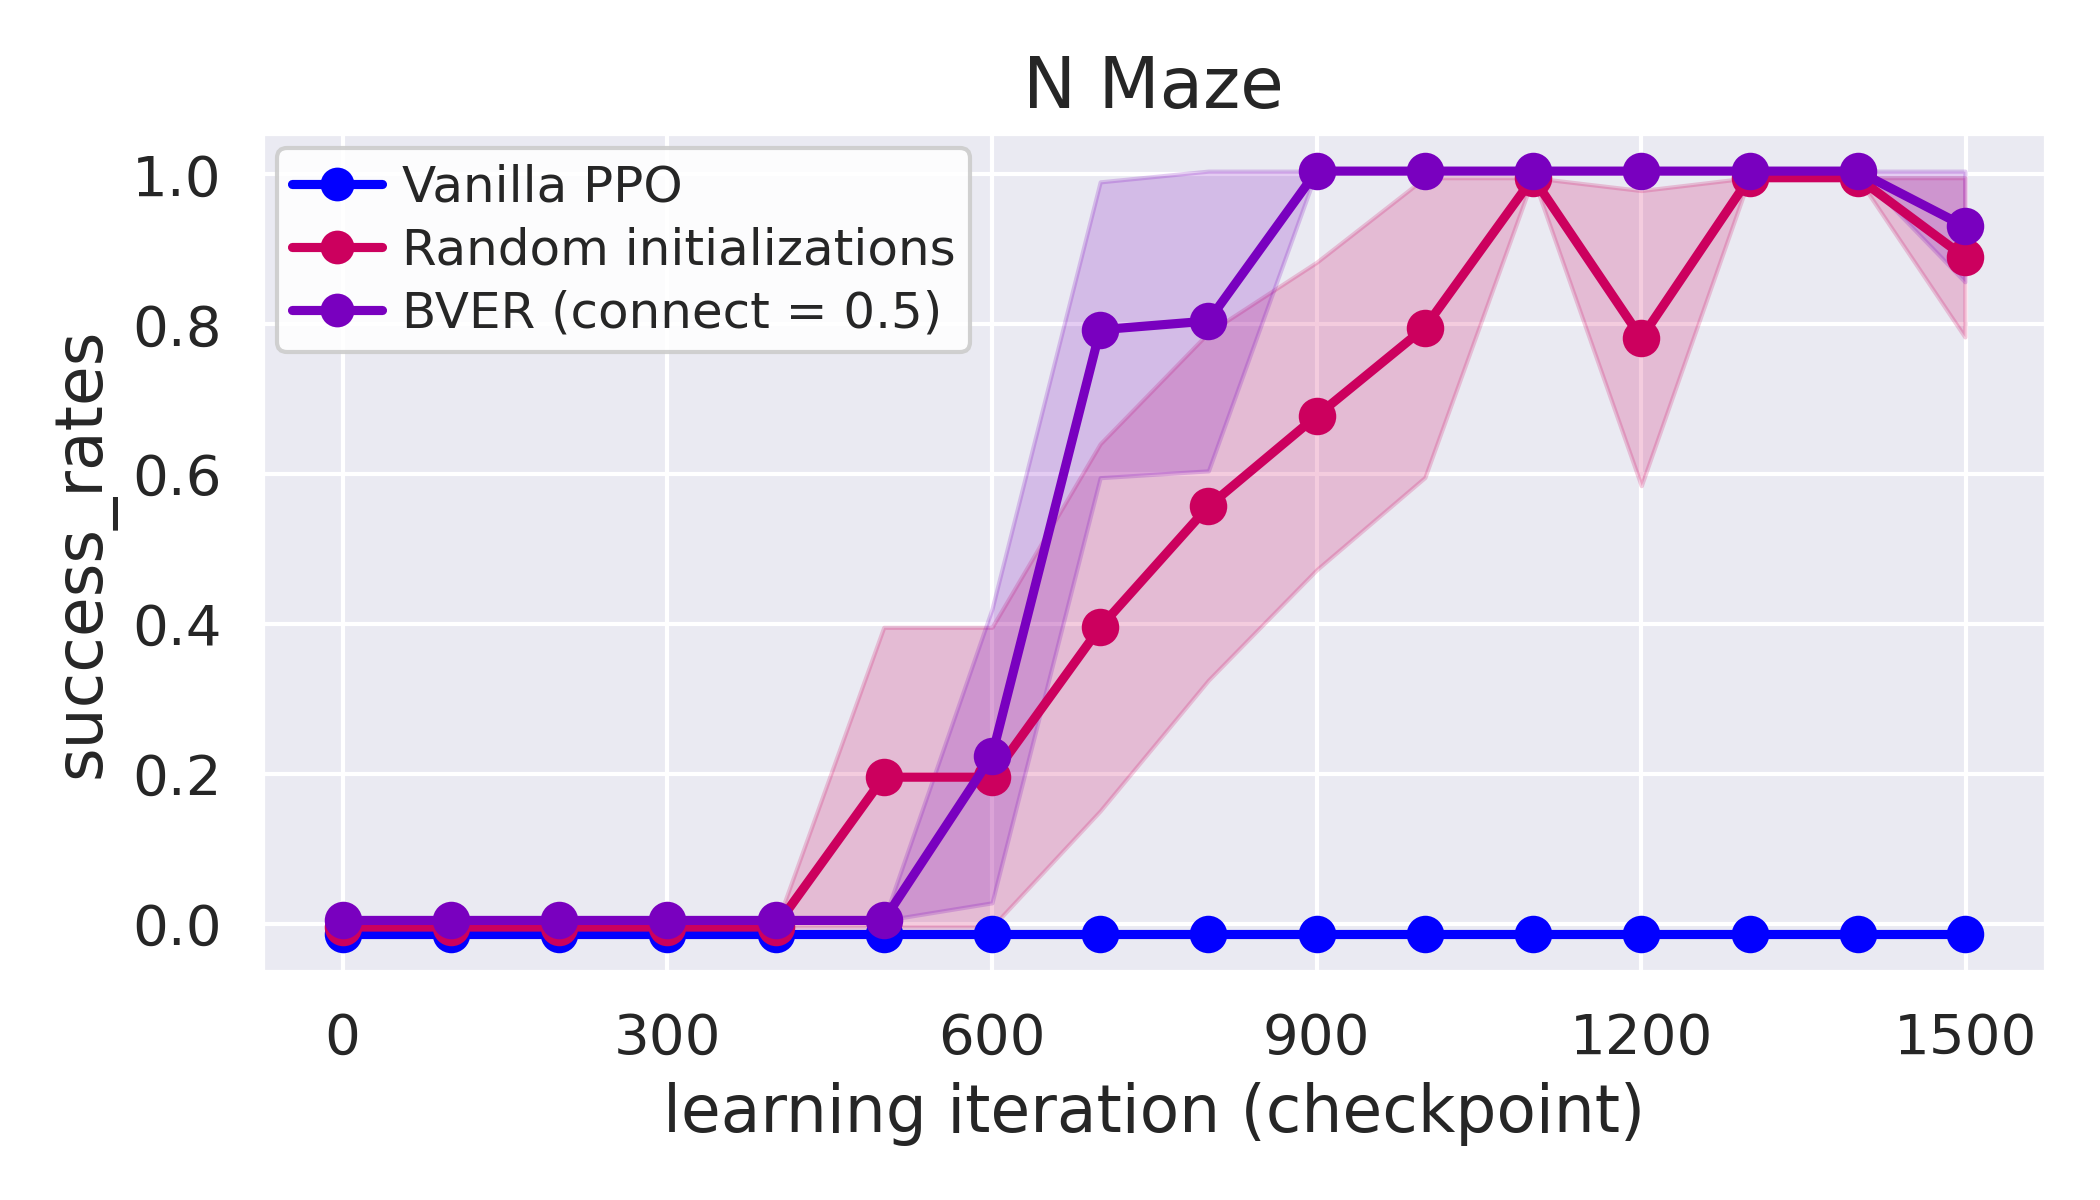
\includegraphics[width=\linewidth]{img/maze/N/eval_comparison_N_maze_bench.png}
    \end{subfigure}
    \hfill
    \begin{subfigure}[c]{0.29\linewidth}
        \centering
        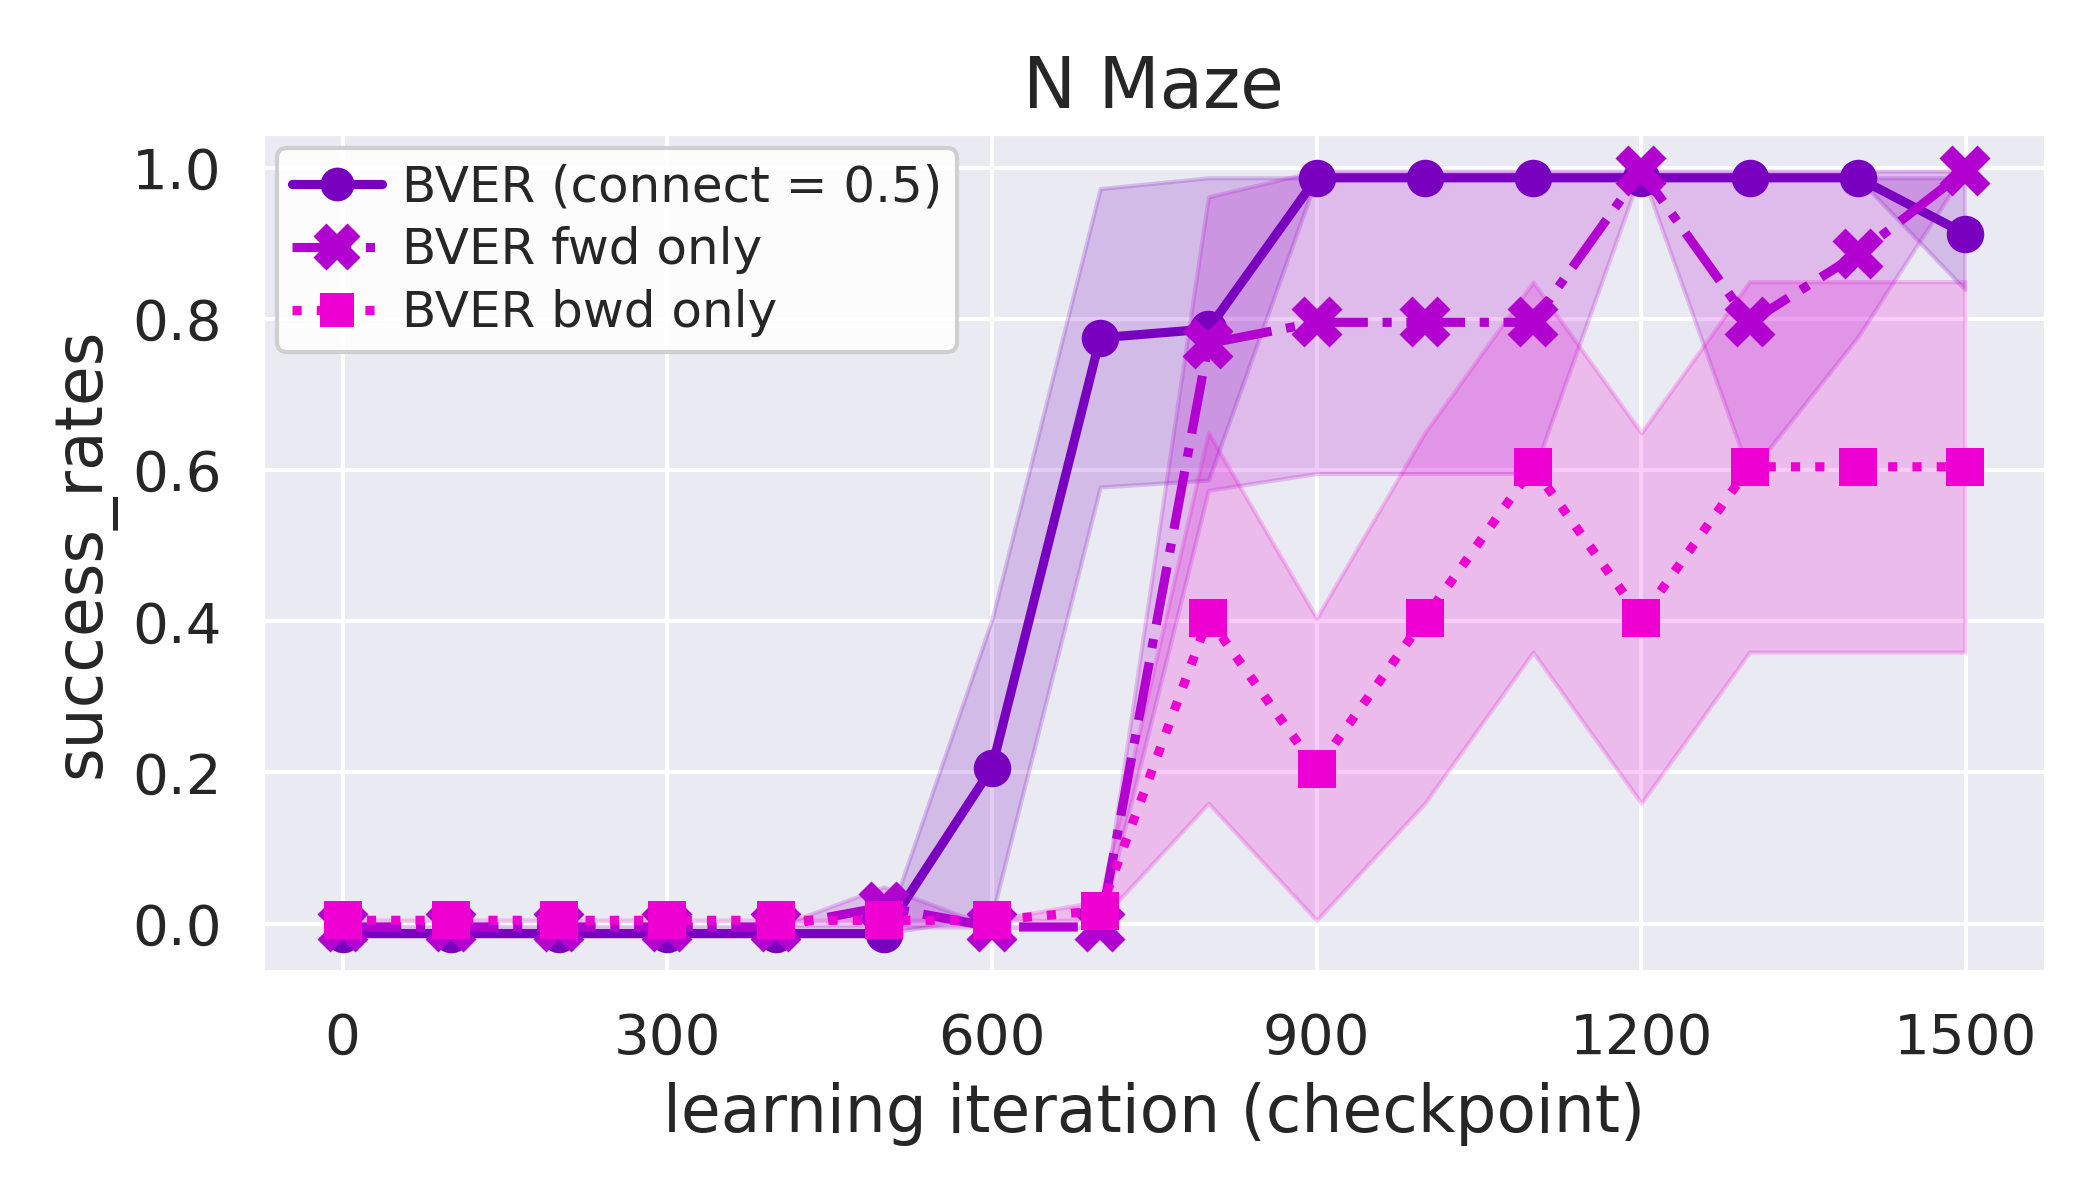
\includegraphics[width=\linewidth]{img/maze/N/eval_comparison_N_maze_abl_dir.png}
    \end{subfigure}
    \hfill
    \begin{subfigure}[c]{0.29\linewidth}
        \centering
        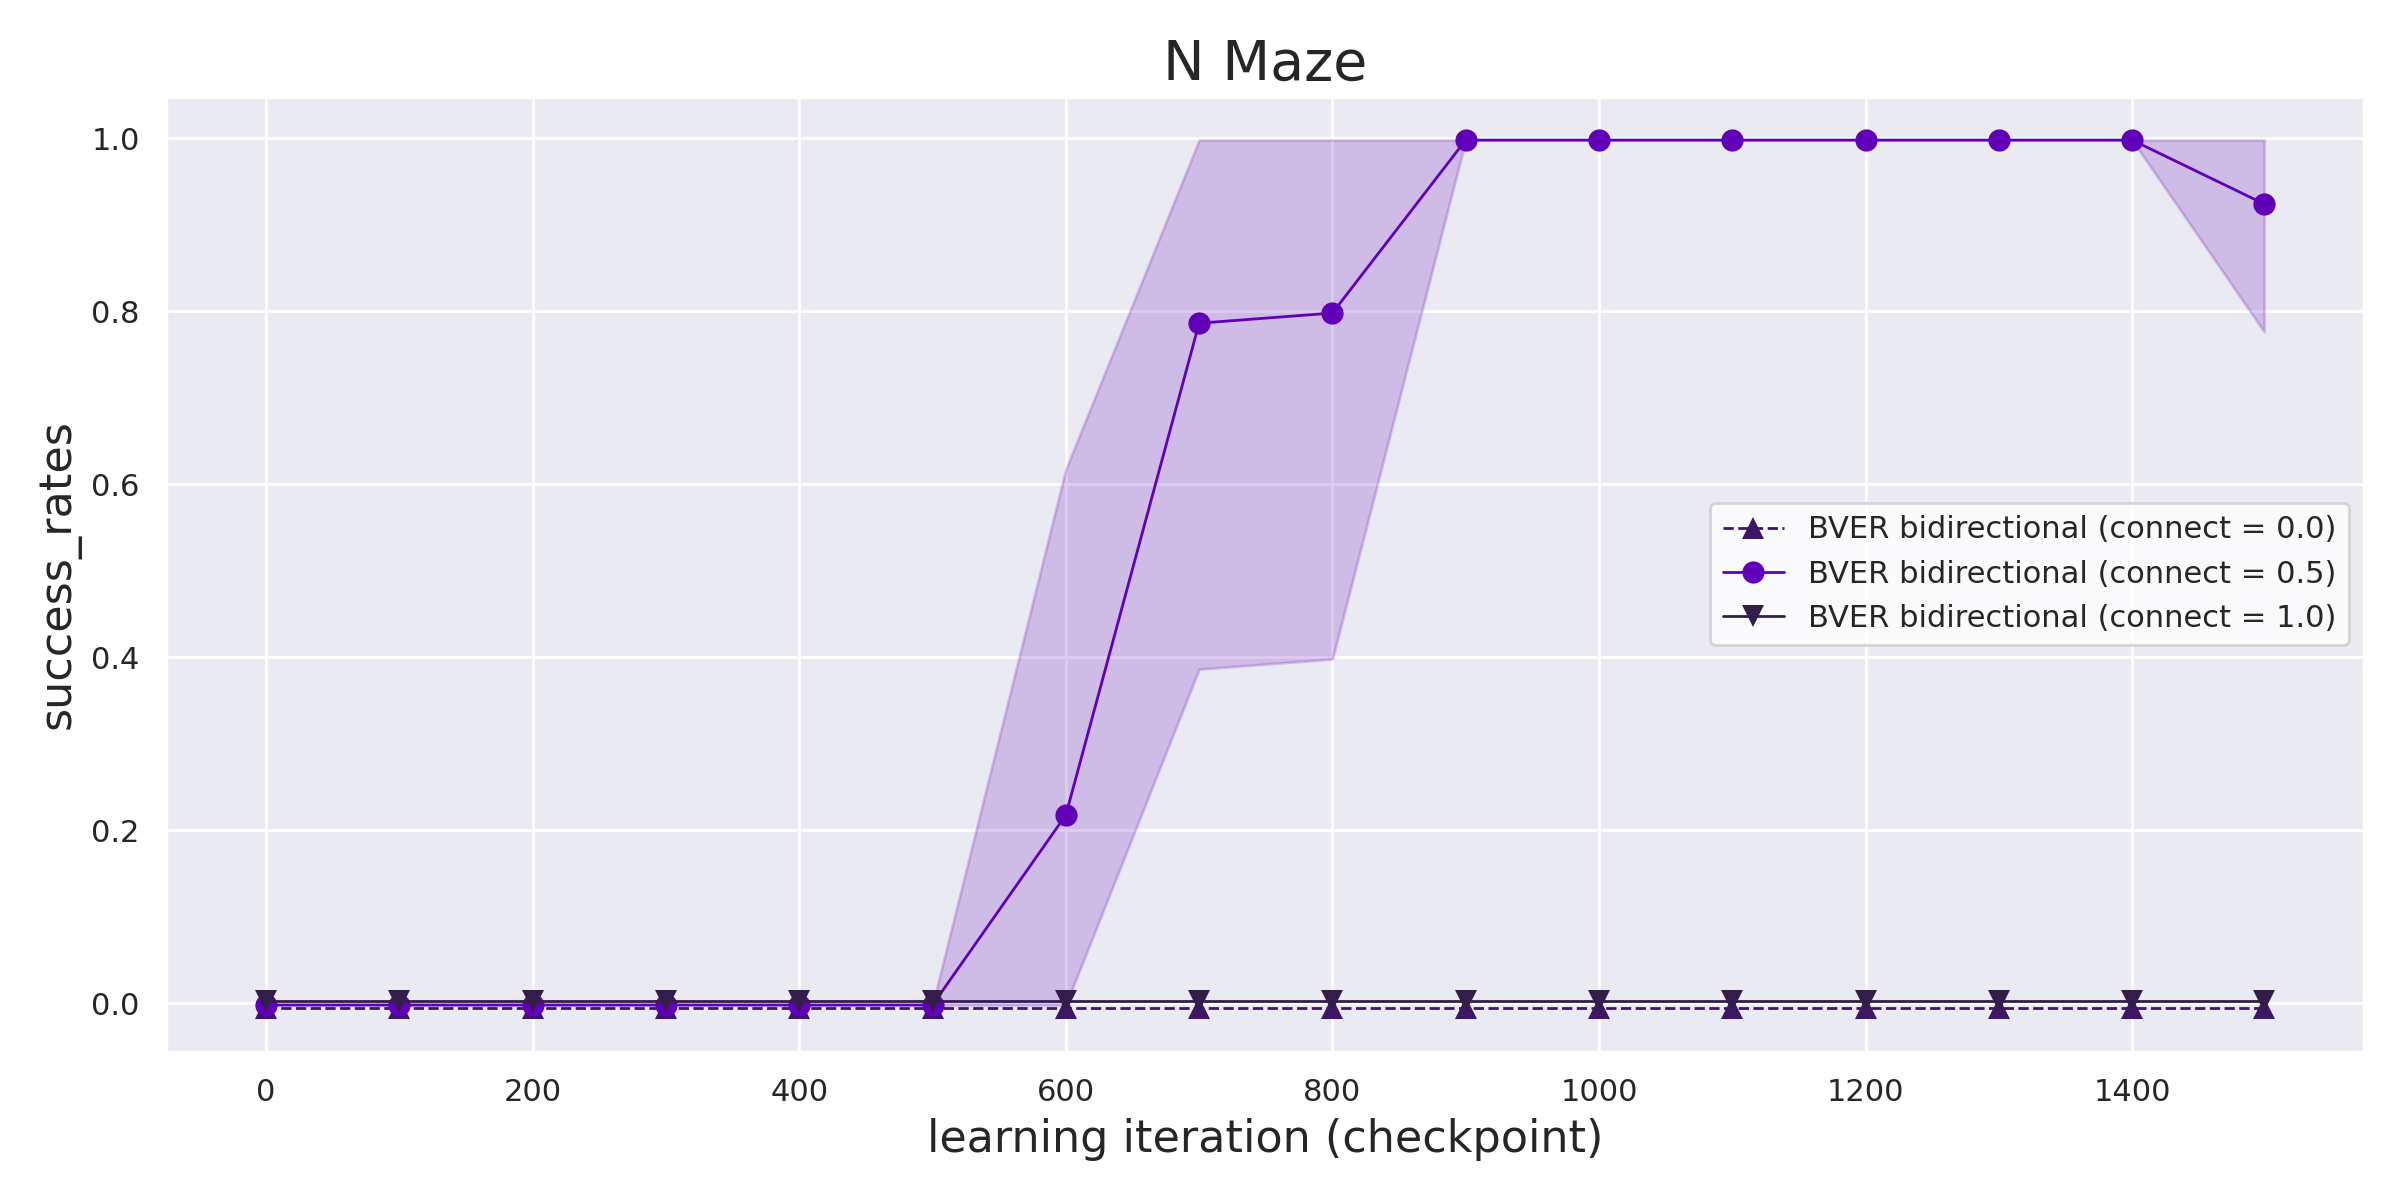
\includegraphics[width=\linewidth]{img/maze/N/eval_comparison_N_maze_abl_connect.png}
    \end{subfigure}
    \hfill\strut{}\\[-2em]
    %
    \hfill
    \begin{subfigure}[c]{0.11\linewidth}
        \centering
        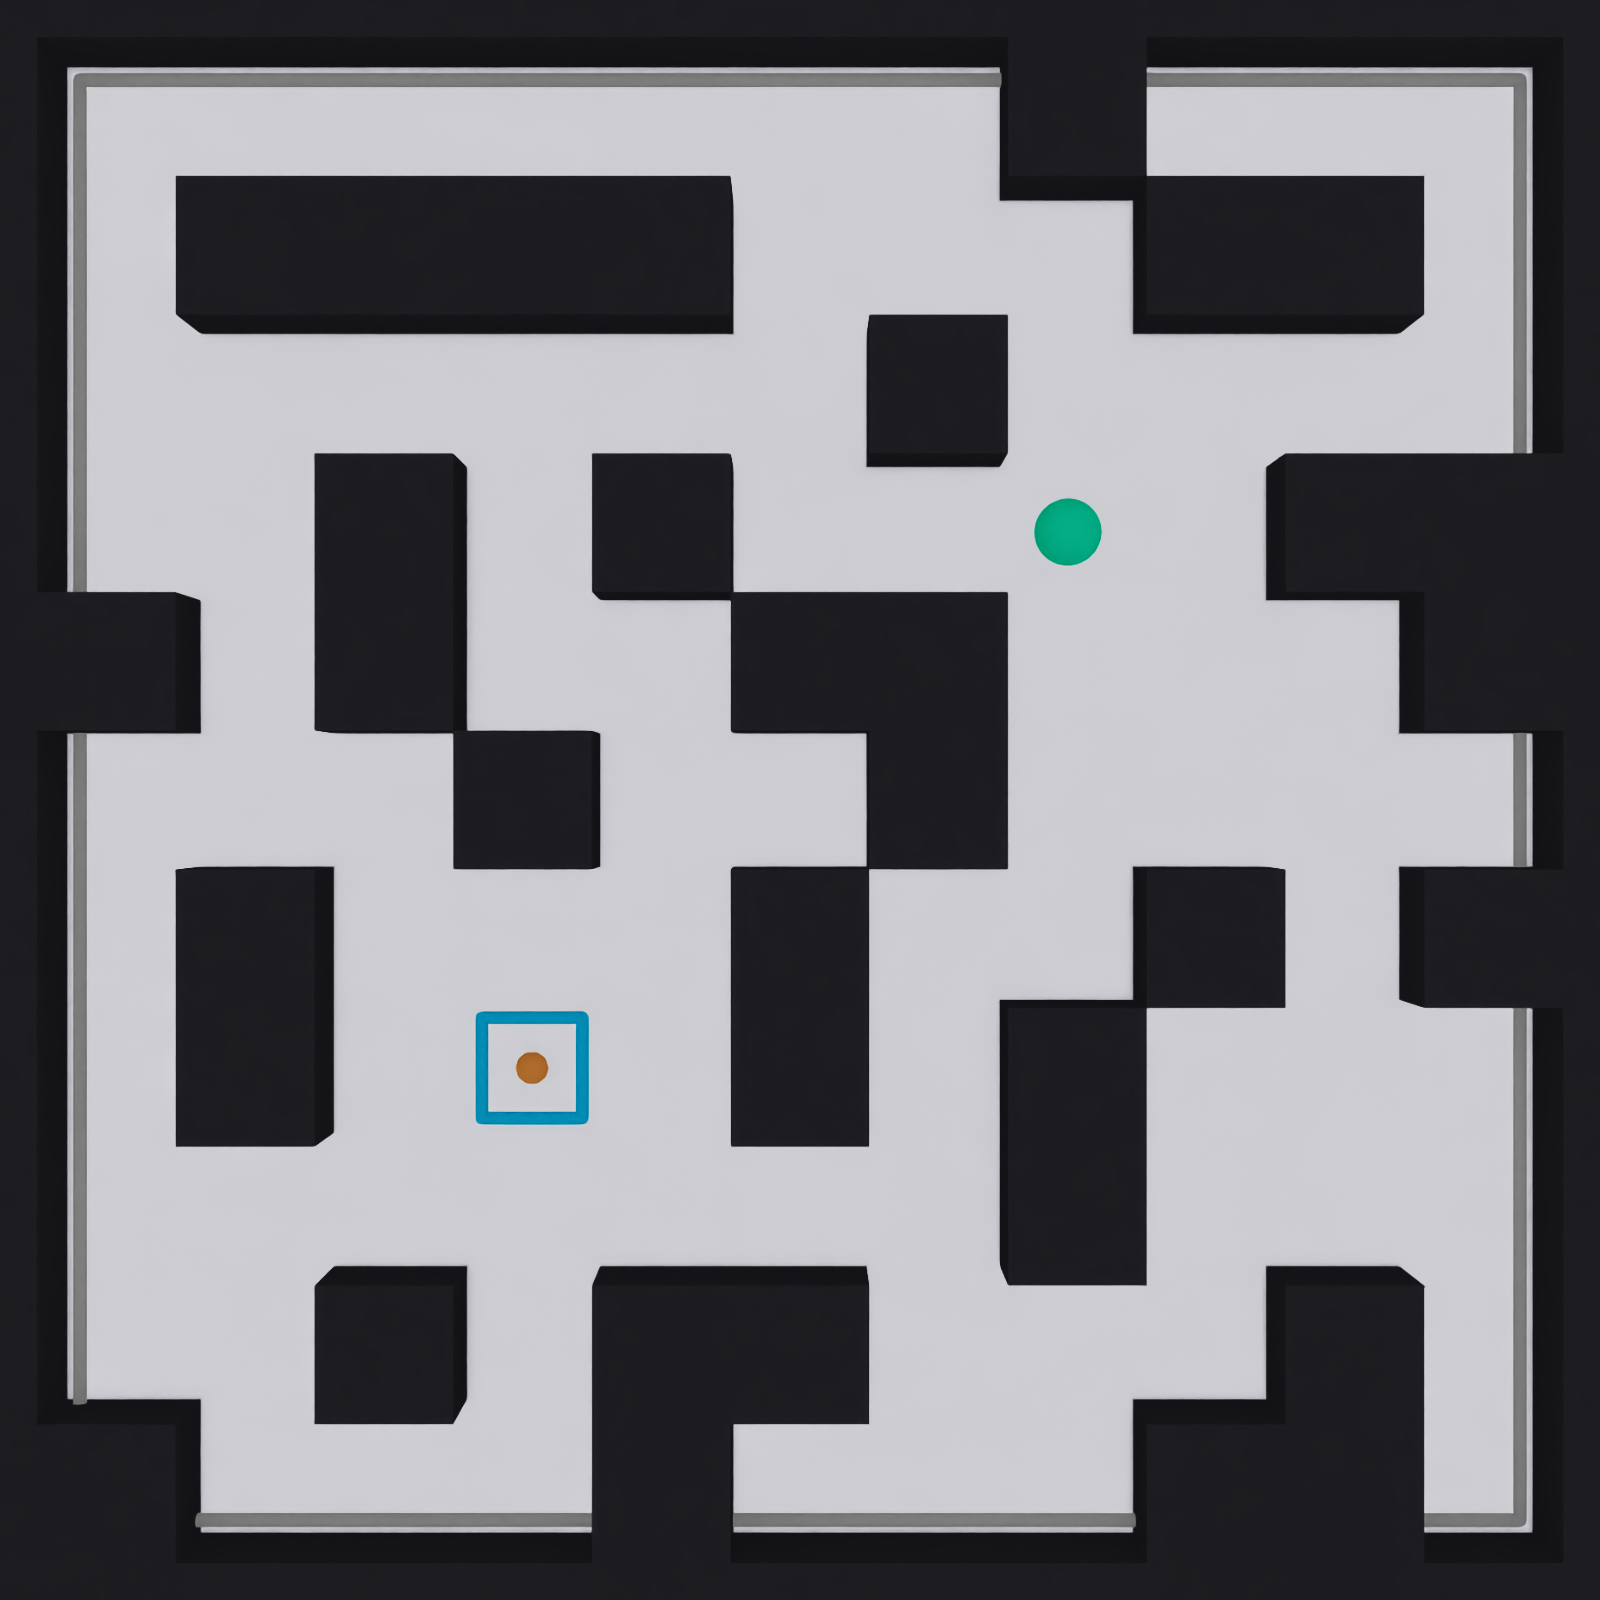
\includegraphics[width=\linewidth]{img/maze/layouts/maze_scatter.png}
        \caption{Maze layout.}\label{fig:maze_layout}
    \end{subfigure}
    \hfill
    \begin{subfigure}[c]{0.29\linewidth}
        \centering
        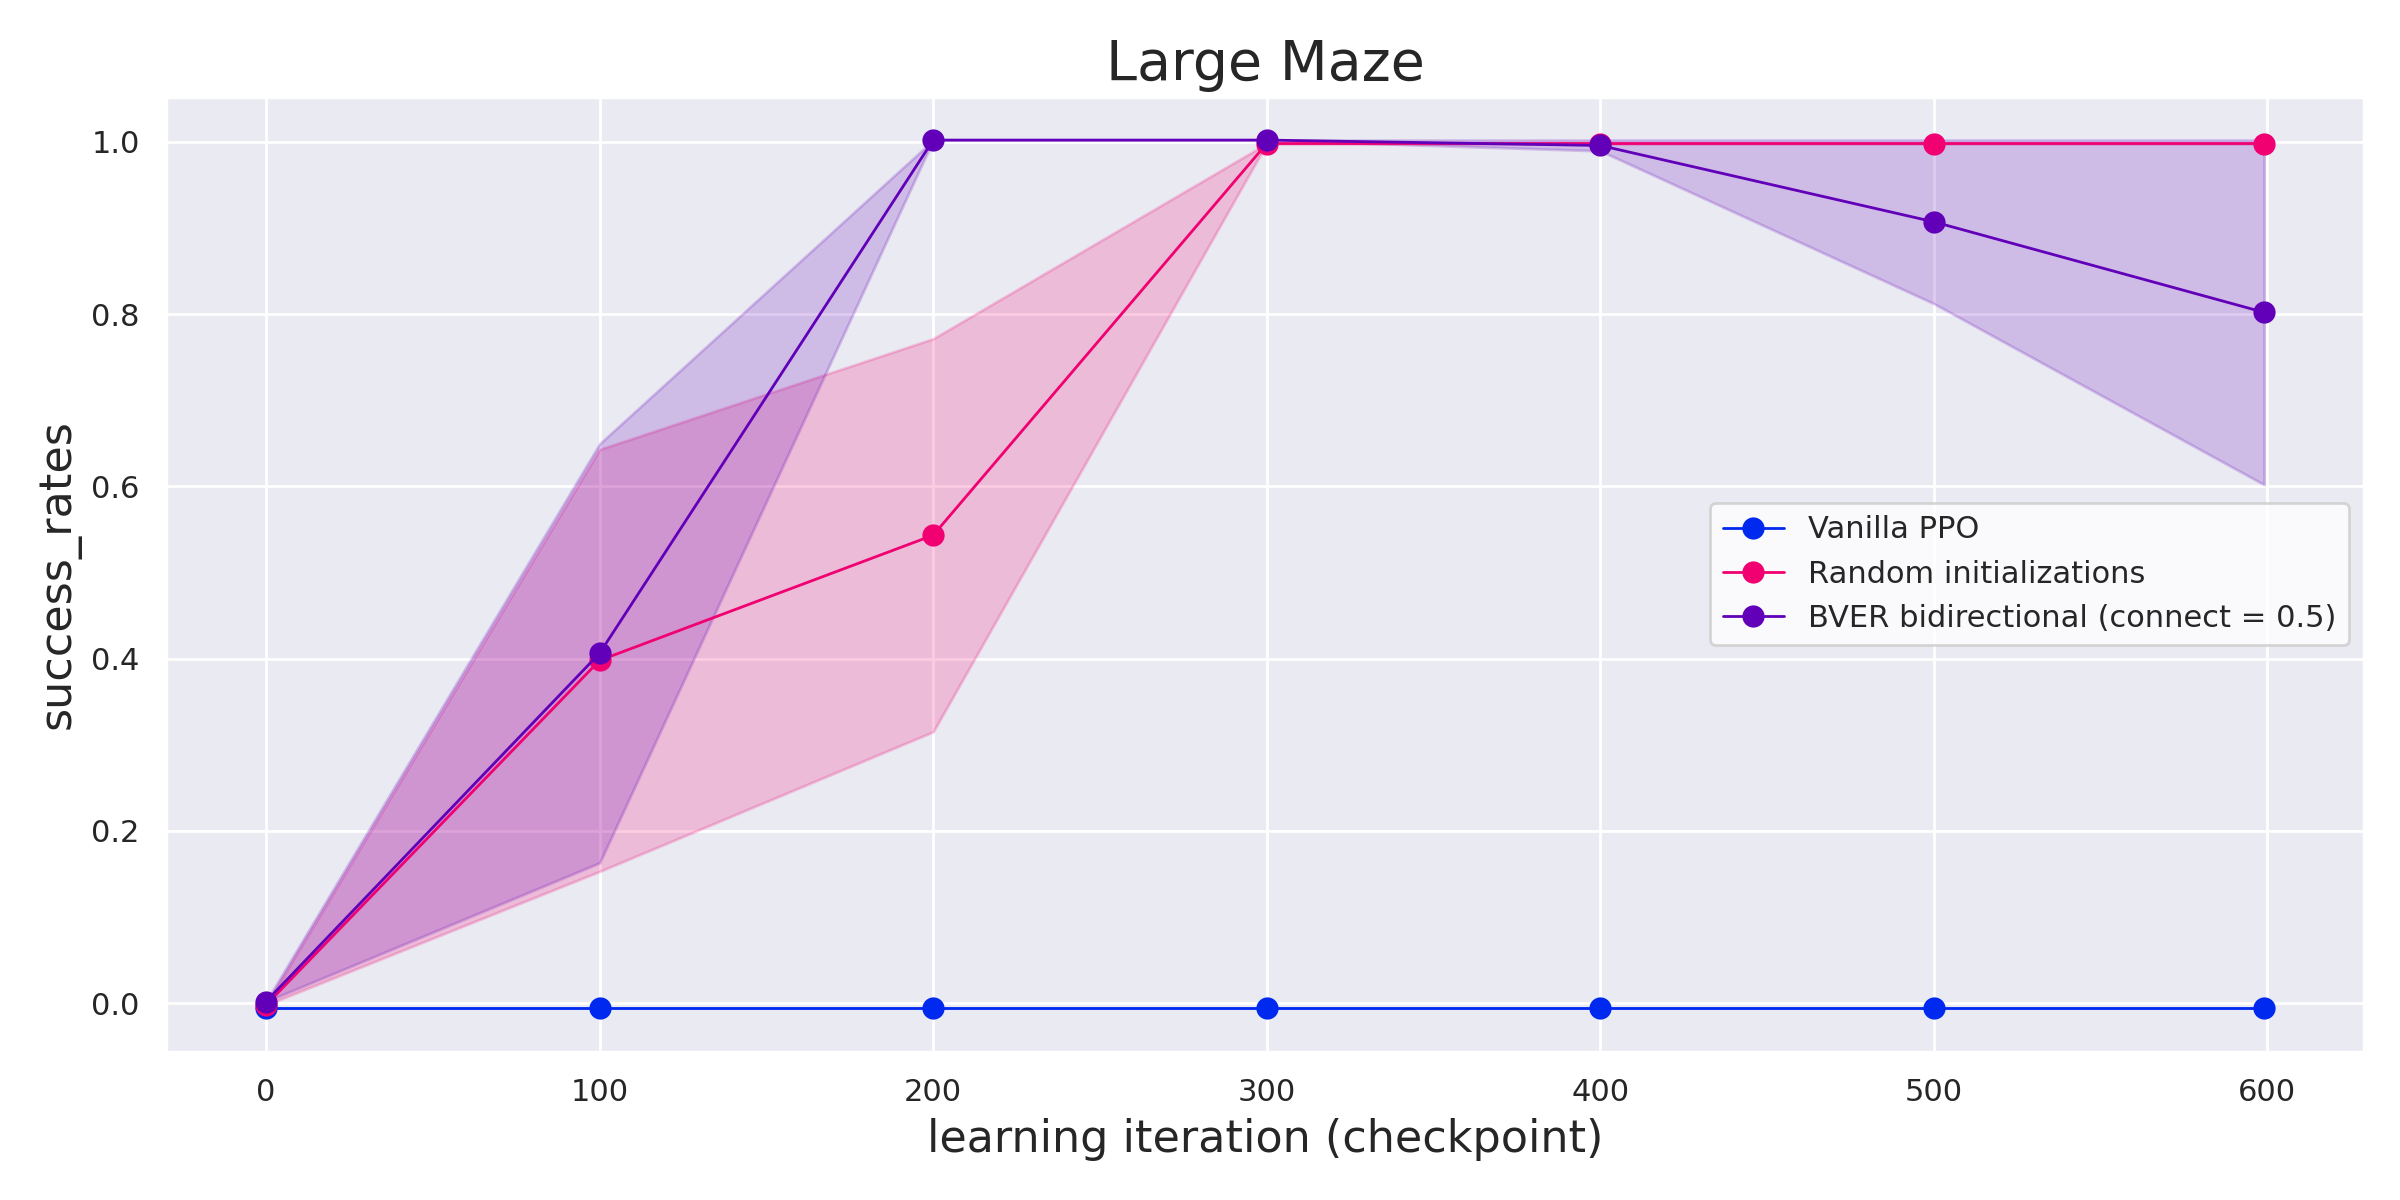
\includegraphics[width=\linewidth]{img/maze/large/eval_comparison_large_maze_bench.png}
        \caption{Benchmark.}\label{fig:maze_ablation_bench}
    \end{subfigure}
    \hfill
    \begin{subfigure}[c]{0.29\linewidth}
        \centering
        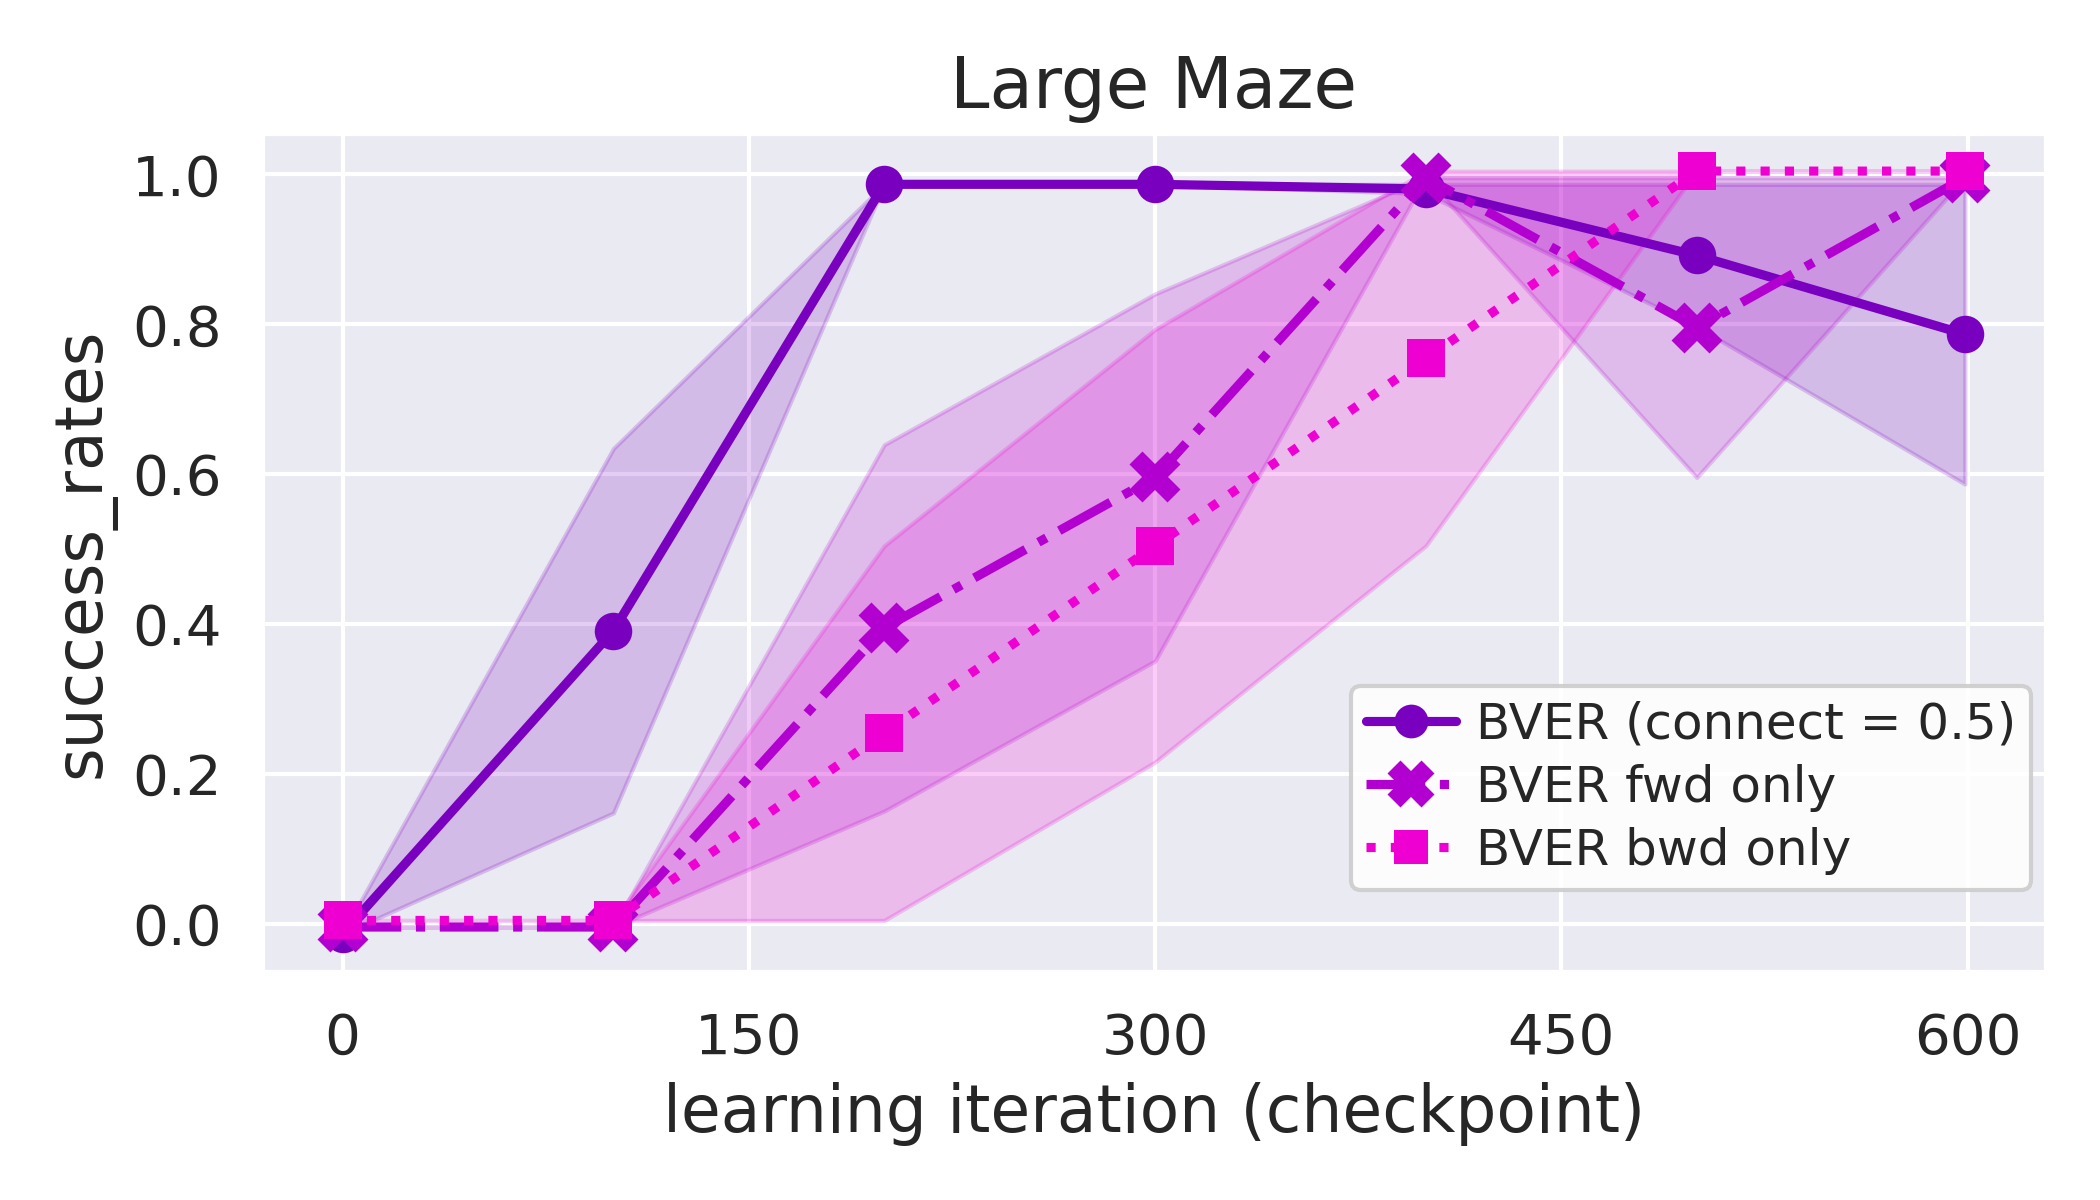
\includegraphics[width=\linewidth]{img/maze/large/eval_comparison_large_maze_abl_dir.png}
        \caption{Direction ablation.}\label{fig:maze_ablation_dir}
    \end{subfigure}
    \hfill
    \begin{subfigure}[c]{0.29\linewidth}
        \centering
        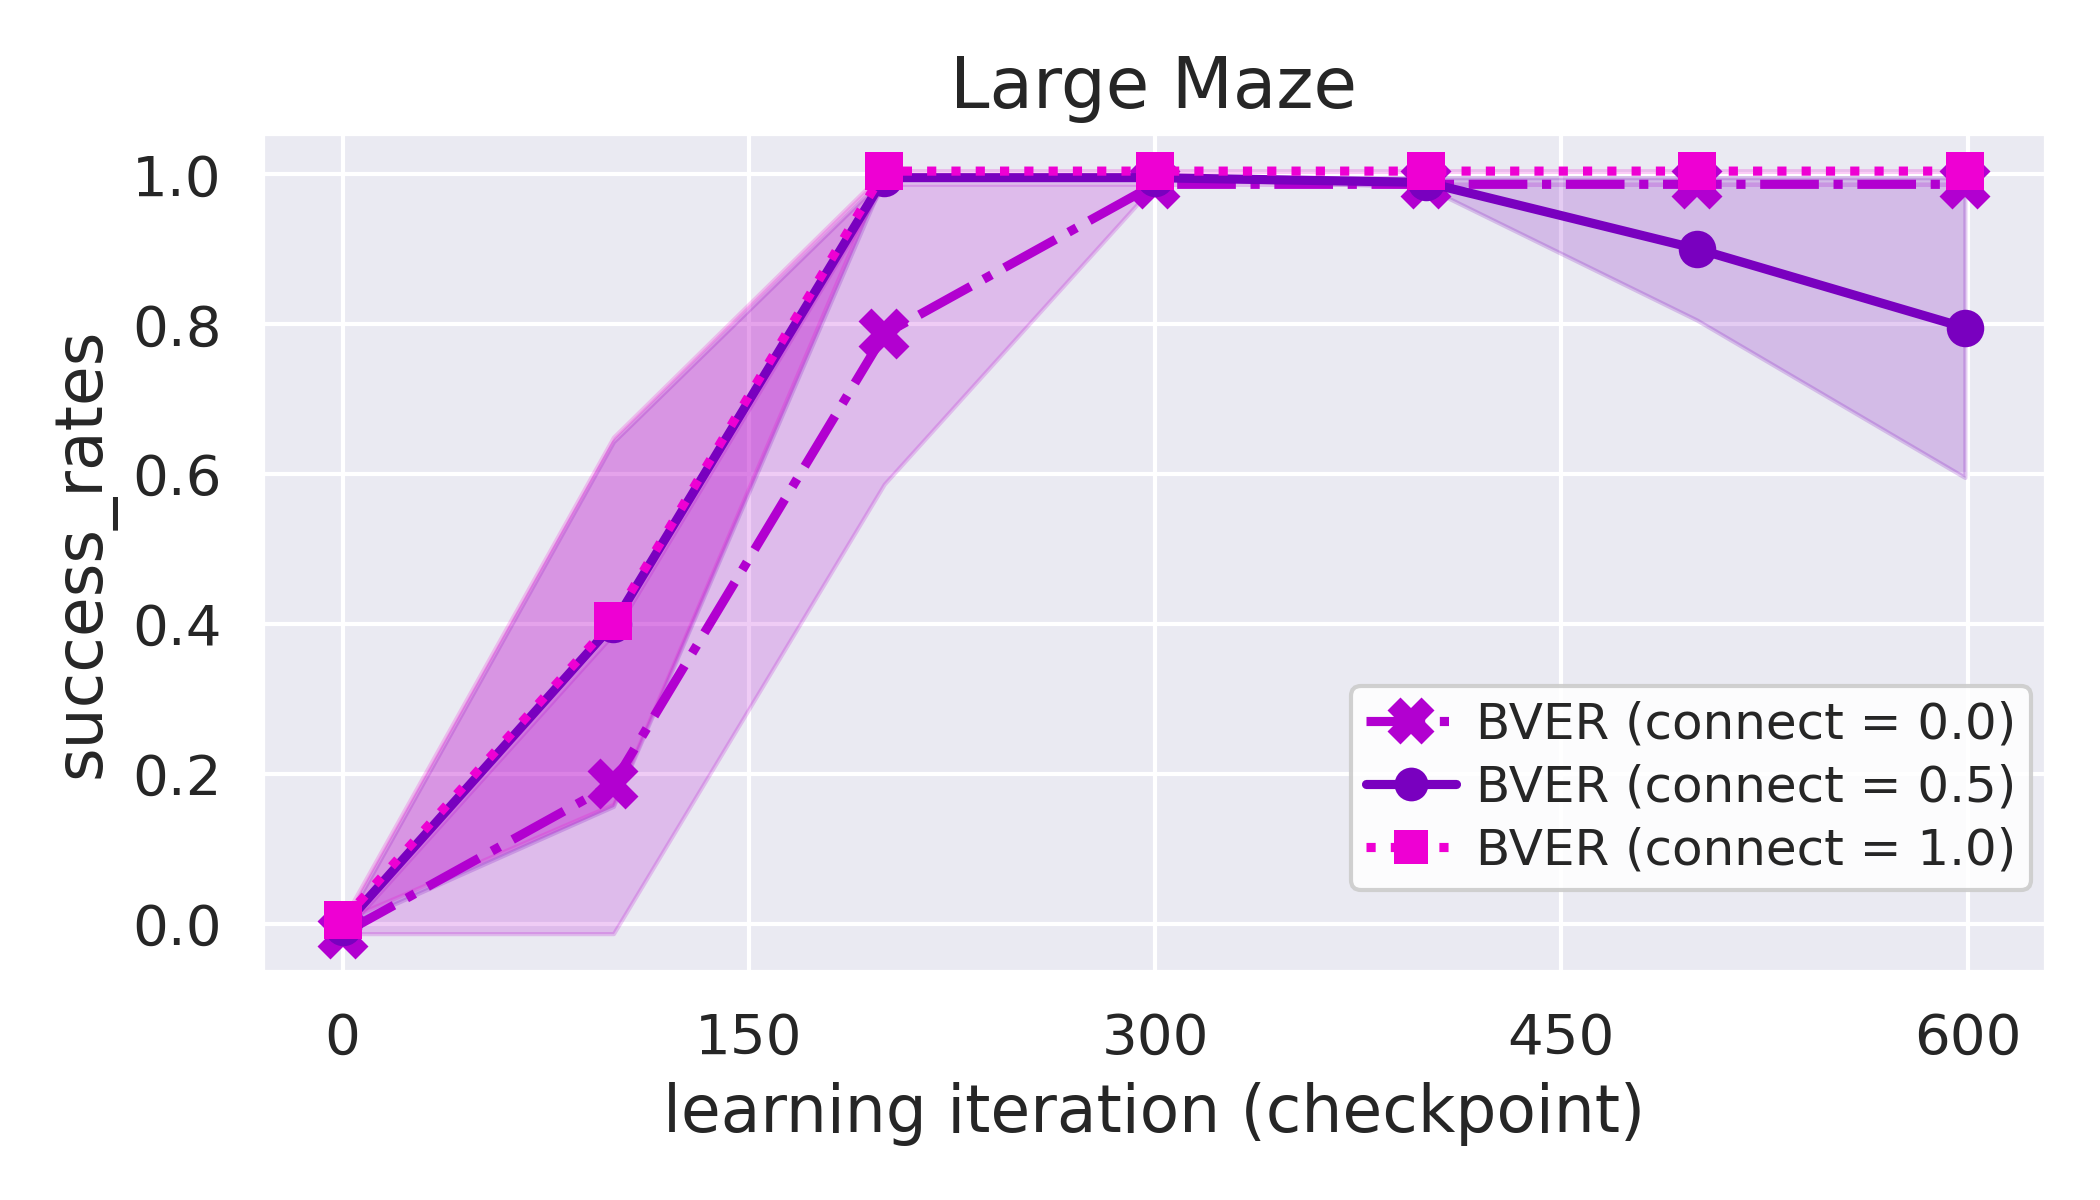
\includegraphics[width=\linewidth]{img/maze/large/eval_comparison_large_maze_abl_connect.png}
        \caption{Connect ablation.}\label{fig:maze_ablation_connect}
    \end{subfigure}
    \hfill\strut{}
    \caption{Comparison of BVER against vanilla PPO and a random curriculum, and ablations of different components (expansion directions) and hyperparameters (connect ratio).}\label{fig:eval_maze_ablations}
\end{figure}

\begin{wrapfigure}{r}{0.55\linewidth}
    \centering
    \vspace{-\baselineskip}
    \begin{subfigure}[b]{0.48\linewidth}
        \centering
        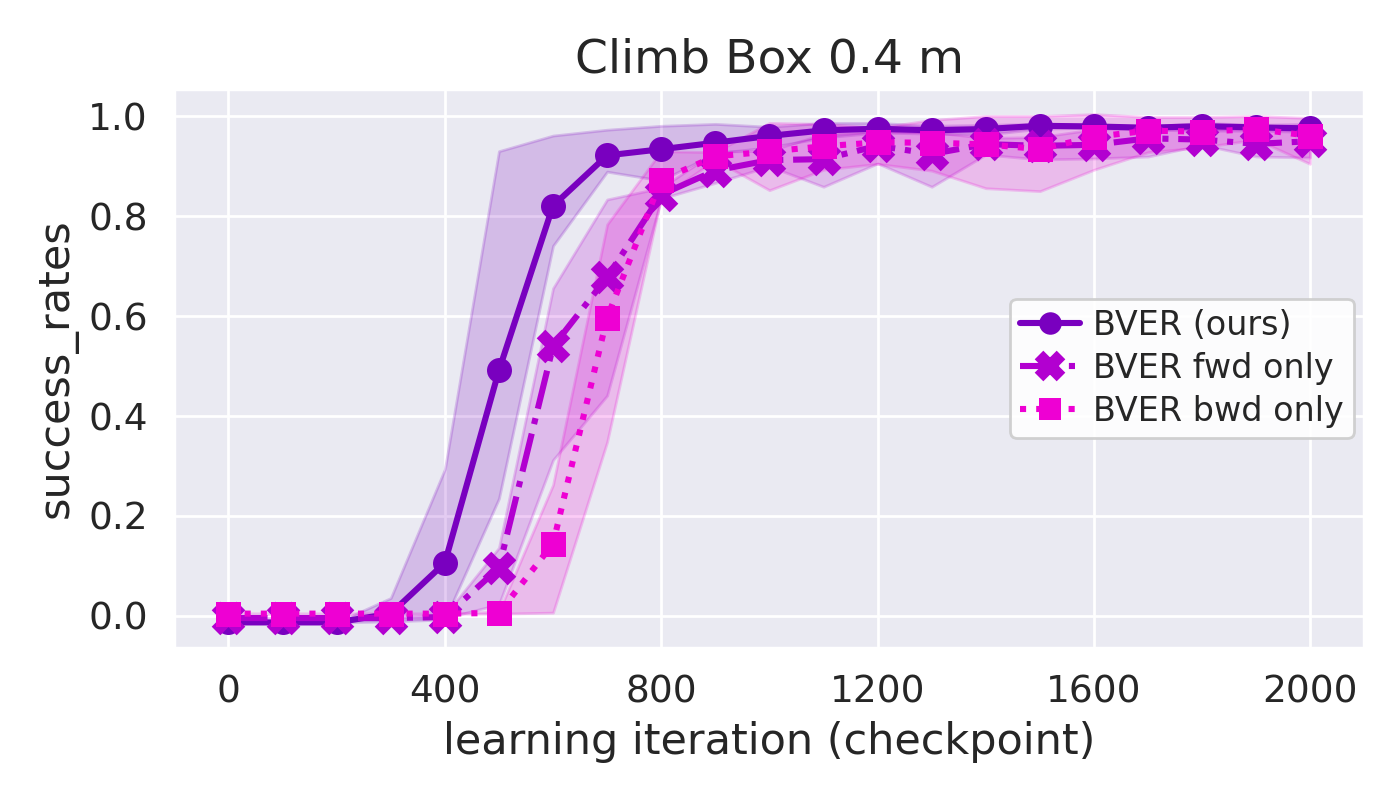
\includegraphics[width=\linewidth]{img/sb/eval_comparison_41_up_ours.png}
        \caption{Climb 0.4 m box up.}\label{fig:eval_comparison_41_up_ours}
    \end{subfigure}
    \hfill
    \begin{subfigure}[b]{0.48\linewidth}
        \centering
        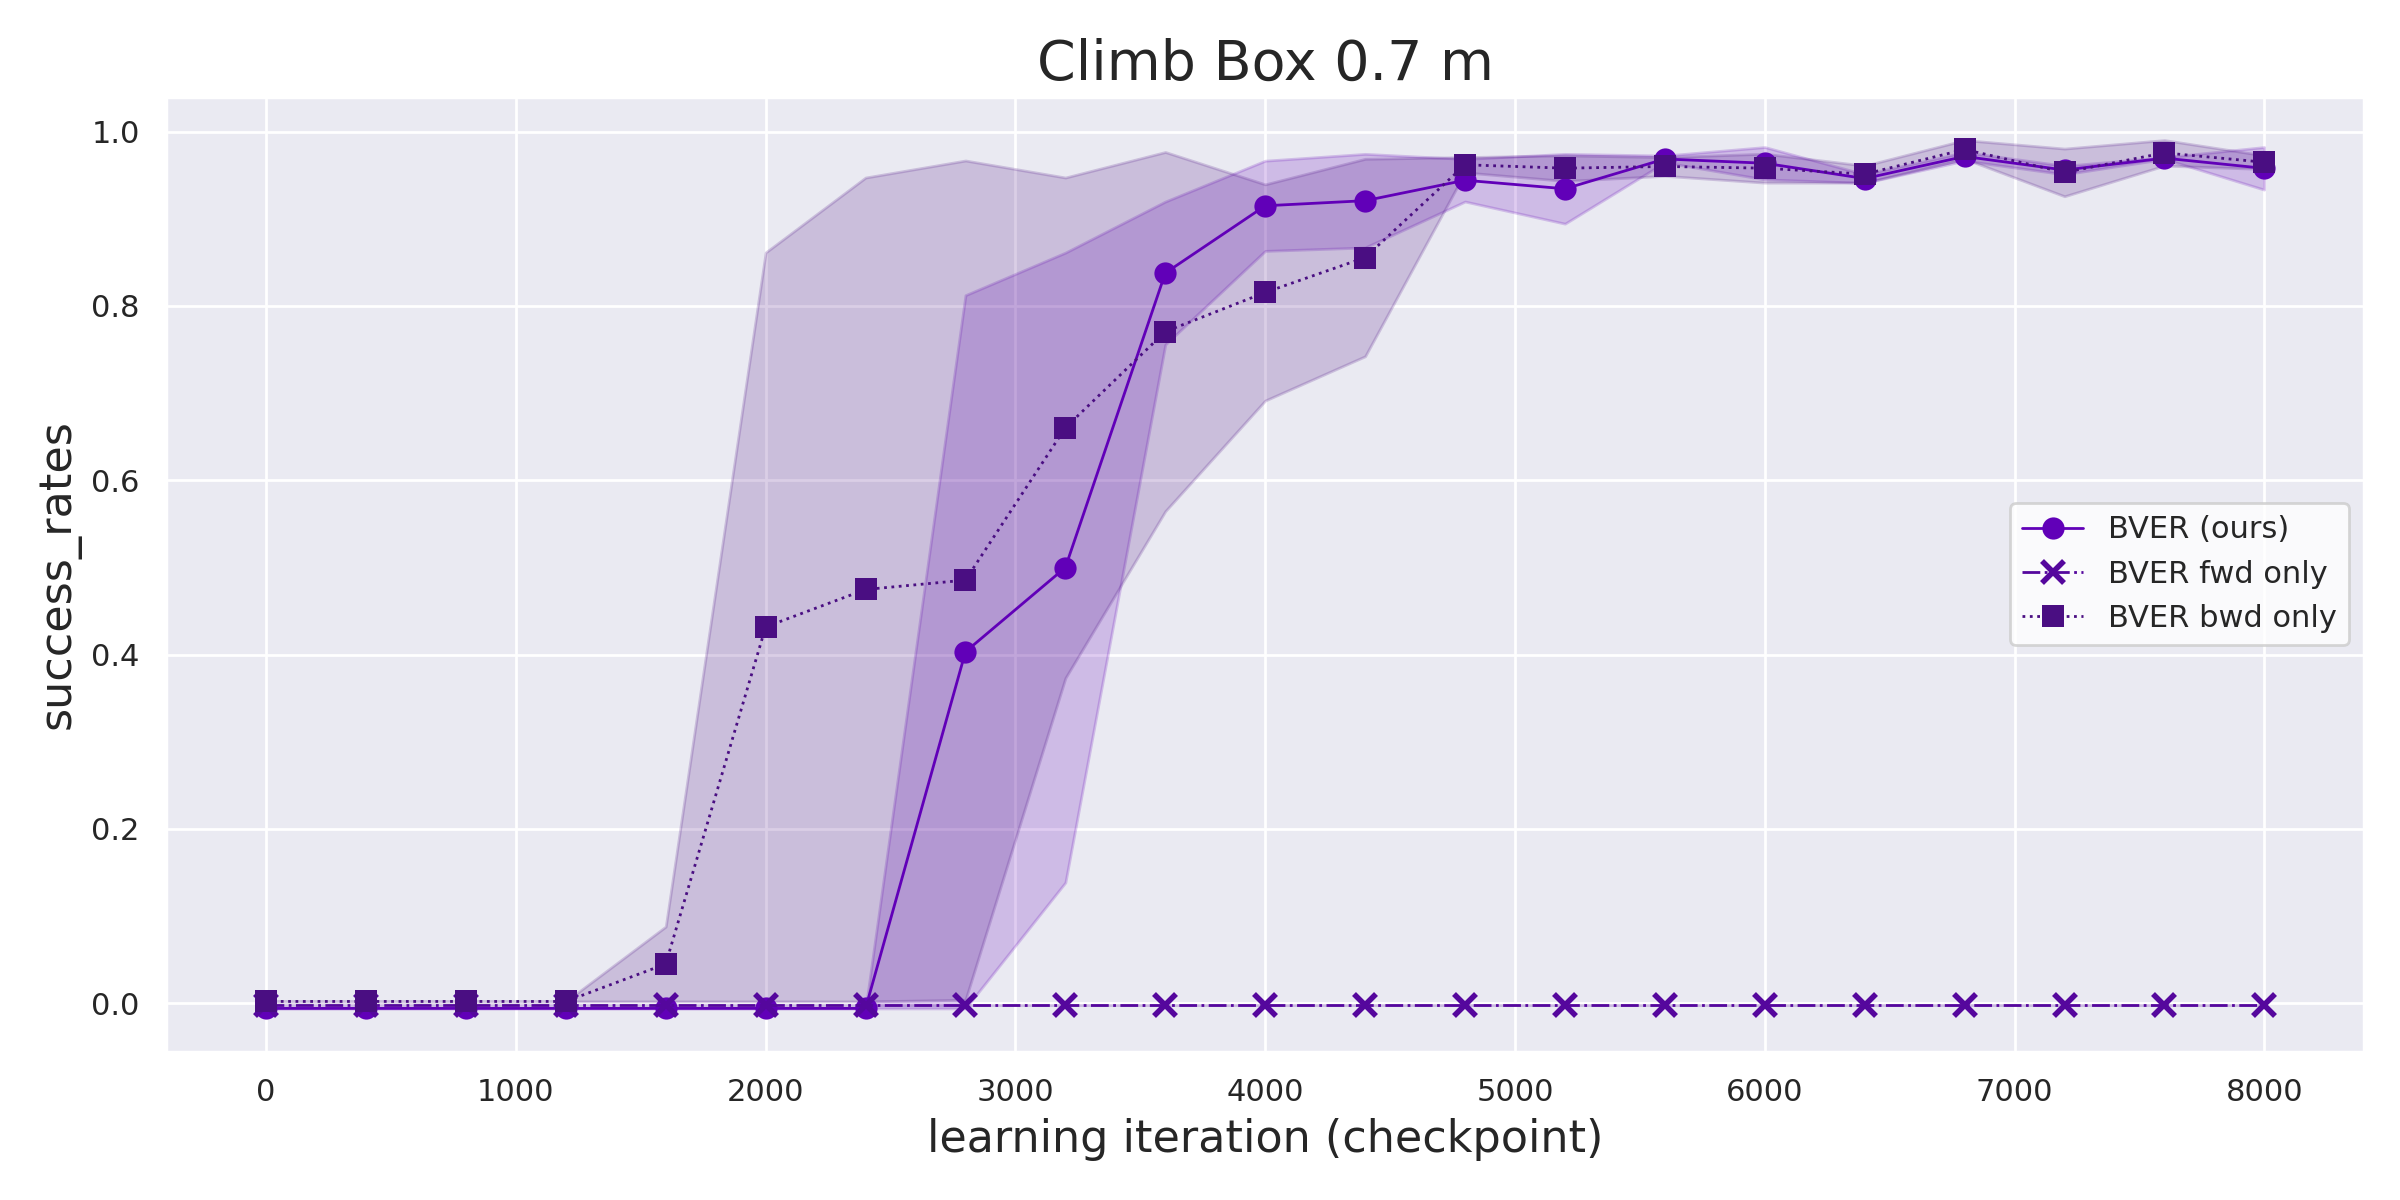
\includegraphics[width=\linewidth]{img/sb/eval_comparison_72_up_ours.png}
        \caption{Climb 0.7 m box up.}\label{fig:eval_comparison_72_up_ours}
    \end{subfigure}
    \\[1ex]
    \begin{subfigure}[b]{0.48\linewidth}
        \centering
        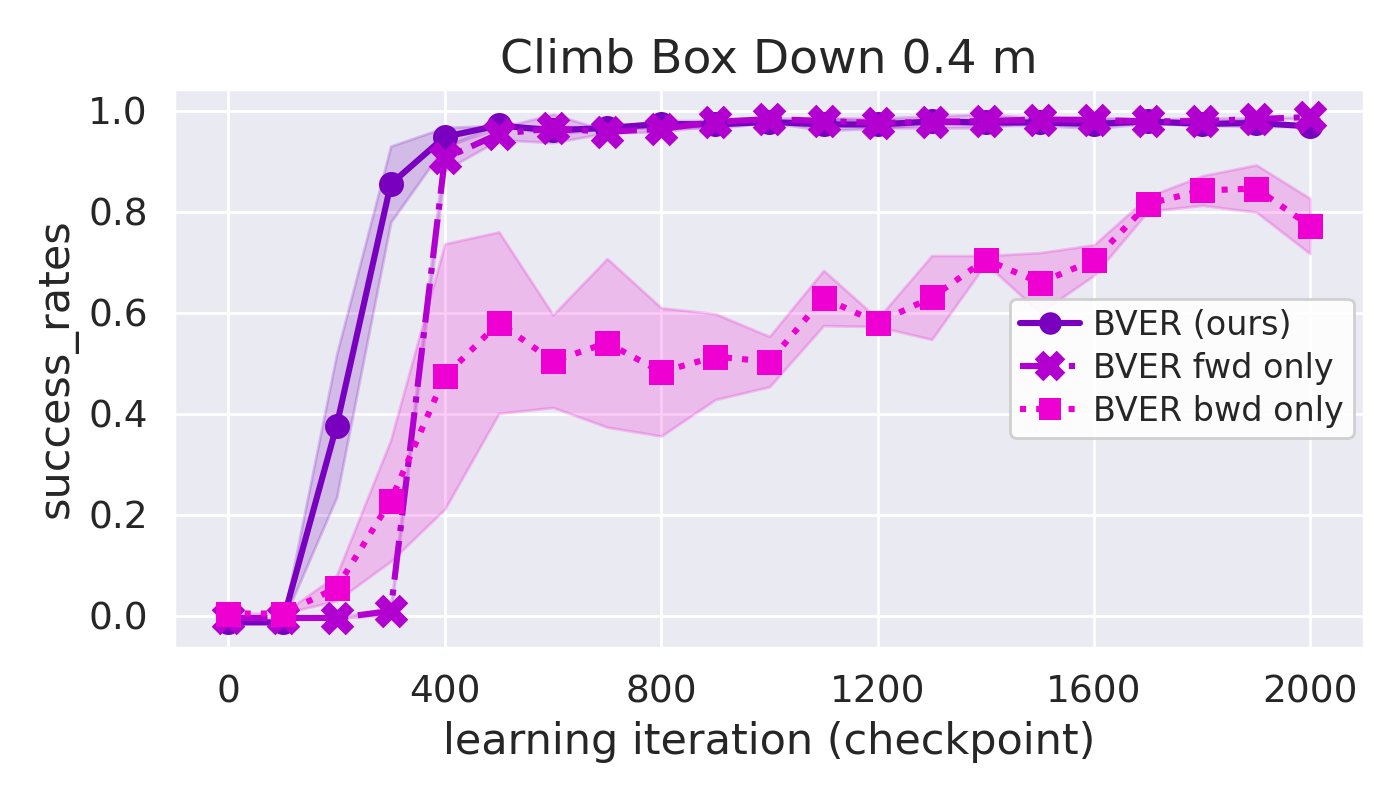
\includegraphics[width=\linewidth]{img/sb/eval_comparison_41_down_ours.png}
        \caption{Climb 0.4 m box down.}\label{fig:eval_comparison_41_down_ours}
    \end{subfigure}
    \hfill
    \begin{subfigure}[b]{0.48\linewidth}
        \centering
        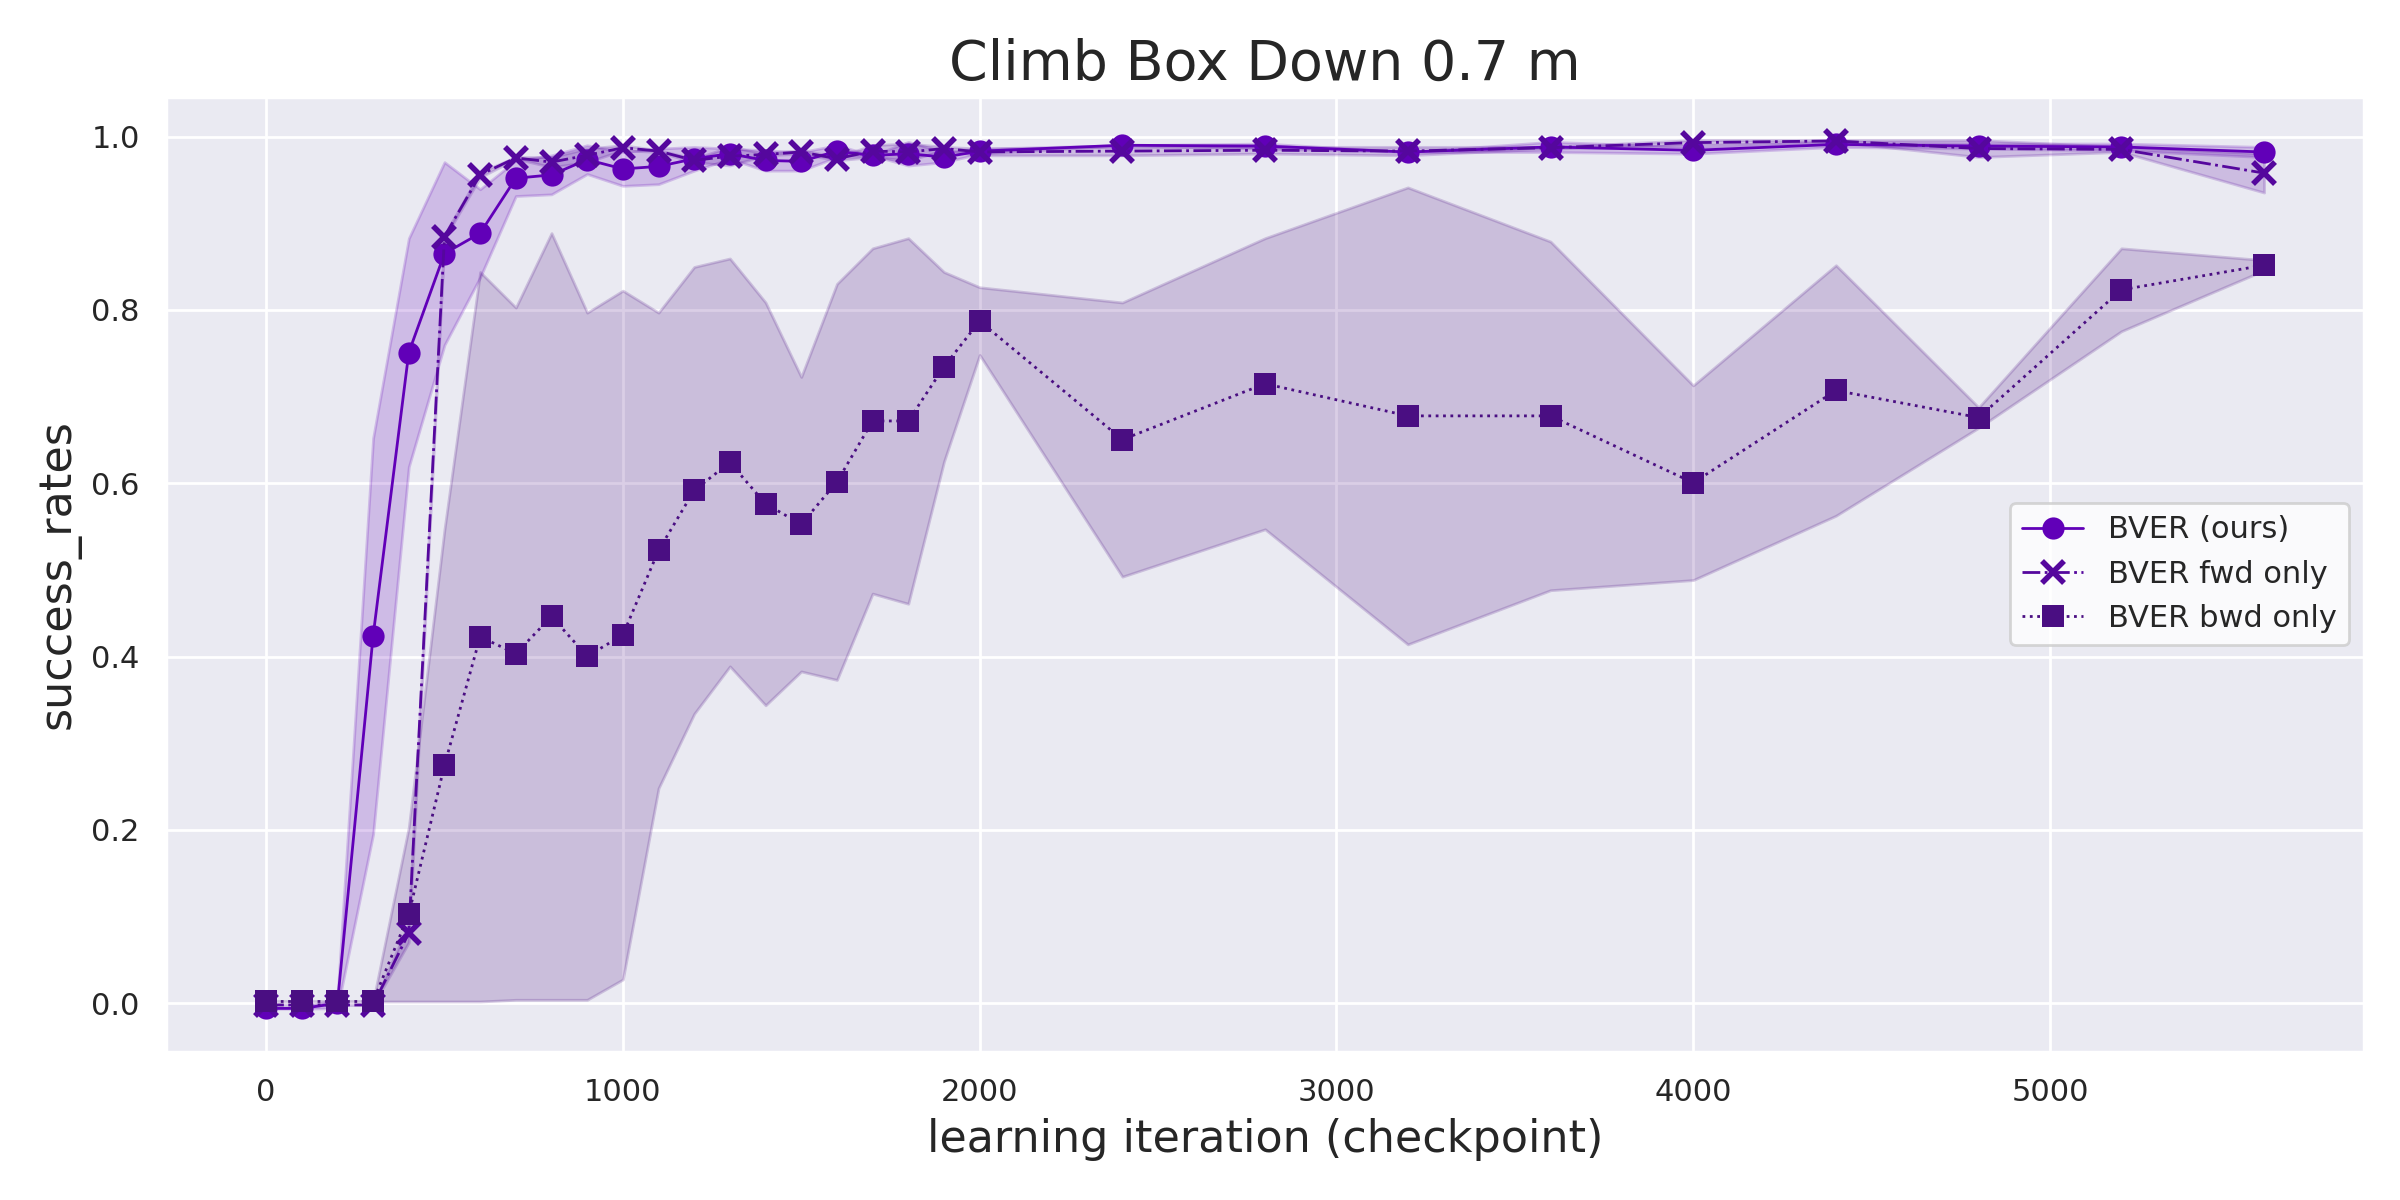
\includegraphics[width=\linewidth]{img/sb/eval_comparison_72_down_ours.png}
        \caption{Climb 0.7 m box down.}\label{fig:eval_comparison_72_down_ours}
    \end{subfigure}
    \caption{Ablations on the box climbing task show that combining forwards and backwards expansions leads to the best results irrespective of direction (up or down) and box height.}\label{fig:eval_ablations}
\end{wrapfigure}
\paragraph{Box climbing ablations:}
We evaluate the effect of the bidirectional expansion mechanism by comparing BVER on two symmetric climbing tasks (up and down) against its unidirectional variants, i.e., only expanding the curriculum from the start state (forwards expansion) or only expanding the curriculum from the goal state (backwards expansion). The results in Figure~\ref{fig:eval_ablations} show that combining forwards and backwards expansions leads to the best results irrespective of the task (up or down) and box height. In both tasks, the expansion that starts on top of the box performs better than the one that starts on the ground. This is likely because the random walks are subject to gravity, so traversing down the box edge is more likely than traversing up it.


\subsection{Emergent Behavior: Path Diversity}\label{sec:exp_emergent}

\begin{wrapfigure}{r}{0.4\linewidth}
    \centering
    \vspace{-\baselineskip}
    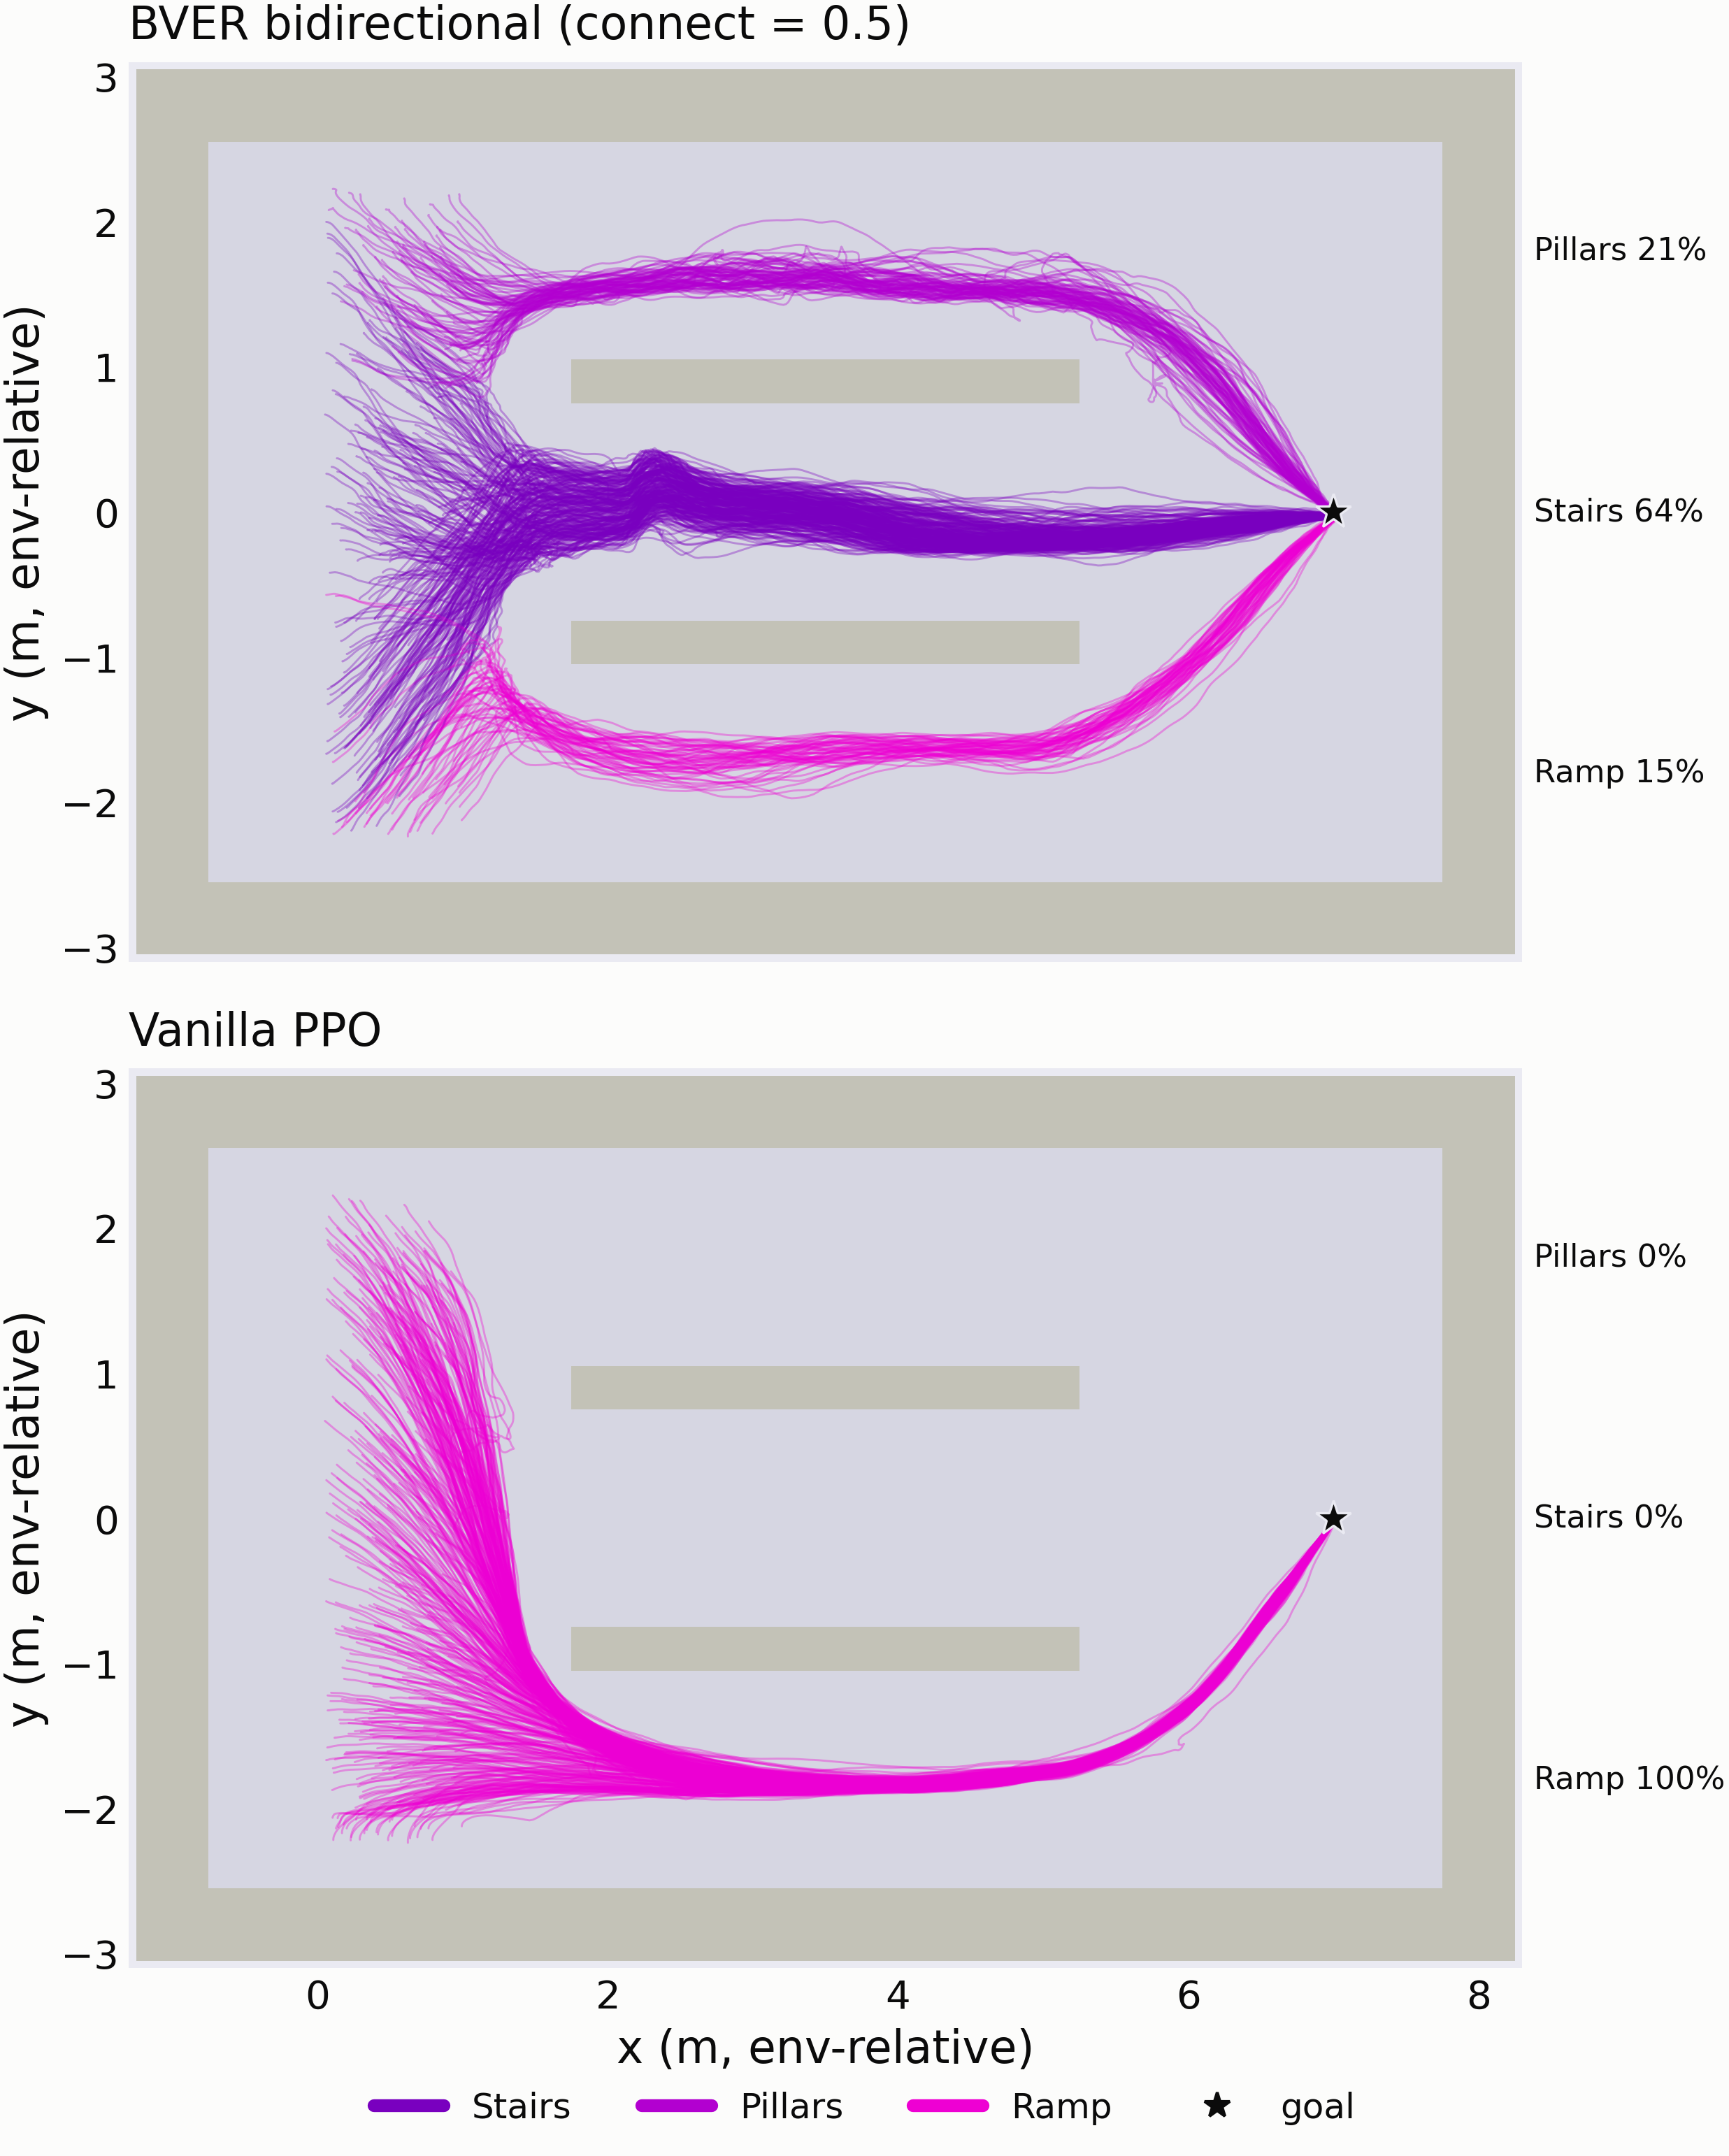
\includegraphics[width=\linewidth]{img/dt/trajectories_model_1999_headline.png}
    \caption{Path diversity on the three-route terrain. PPO without a curriculum collapses onto the ramp, while BVER learns to traverse all three routes.}\label{fig:eval_path_diversity}
\end{wrapfigure}

To answer research question 3, we design a task with three qualitatively different routes from the initial distribution to the goal: a set of stairs in the center, a field of pillars on one side, and a ramp on the other (Figure~\ref{fig:exp_renders_dtsg}). The initial distribution is chosen to span the full width of the terrain, such that each of the three routes is the closest one for roughly a third of the initial states and no route is favored. After training, we roll out both policies from this broad initial distribution and classify every successful episode by the route it takes.

Figure~\ref{fig:eval_path_diversity} shows that PPO without a curriculum collapses onto a single behavior: all successful episodes traverse the ramp, which is the easiest but not necessarily the shortest route, regardless of where the episode starts. Once this route is discovered, exploration of the remaining task space stops, and the policy never learns to climb the stairs or navigate the pillars, even when it is initialized directly in front of them. In contrast, BVER's task-space coverage-driven expansion forces the curriculum to remain active in all regions of the task space, and the resulting policy uses all three routes, choosing the one closest to its initial state. This indicates that task-space coverage promotes more diverse learning outcomes: rather than committing to the first solution it finds, the policy acquires the full set of locomotion skills the terrain affords, which makes it less dependent on any single route being available.

\subsection{Real-World Terrains}\label{sec:exp_real_world}

To show its practical applicability and answer research question 4, we evaluate BVER on four different real-world terrains with the ANYmal D quadrupedal robot in an identical setup to the box climbing task in Section~\ref{sec:exp_main}. We use the same hyperparameters and curriculum settings as in the box climbing task, and choose the task space to roughly cover the terrain area. The four terrains in Figure~\ref{fig:experiment_renders} can be categorized as follows: (1) climbing a freestanding boulder (Figures~\ref{fig:exp_renders_freestanding_boulder_I} and~\ref{fig:exp_renders_freestanding_boulder_II}), (2) traversing over a field of small stones (Figure~\ref{fig:exp_renders_small_rocks}), and (3) ascending a steep rocky slope (Figure~\ref{fig:exp_renders_rocky_ascent}), each requiring different locomotion skills. On the \textit{freestanding boulders} and the \textit{small stone field}, the initial distribution is chosen such that no specific path to the goal is favored and the policy has to find its own path to the goal. Table~\ref{tab:real_world_results} shows that, similar to box climbing, PPO without a curriculum is unable to solve the task, while BVER finds solutions in reasonable time on all four terrains.
% \renewcommand{\arraystretch}{1.3}
\begin{table}[h]
    \centering
    \caption{Training iterations needed to reach a success rate of 95\% on the four real-world terrains.}\label{tab:real_world_results}
    \begin{tabularx}{\linewidth}{@{}rcccc@{}}
        \bf Task    & Freestanding boulder I & Freestanding boulder II & Small stone field & Rocky ascent \\
        \cmidrule{2-5}
        Vanilla PPO & --                     & --                      & --                & --           \\
        BVER        & $1800\pm x$            & $2300\pm x$             & $2500\pm x$       & $3500\pm x$  \\
    \end{tabularx}
\end{table}
% \renewcommand{\arraystretch}{1}

Figure~\ref{fig:scans} shows the explored regions on the \textit{rocky ascent} terrain at different training iterations. The intermediate starts and goals are clustered around their respective roots at the beginning of training, and gradually expand to cover the entire task space as the policy's skill improves. Even though the task space (black/white box) is much larger than the reachable area of the robot, the curriculum is able to find a path to the goal without any prior knowledge of the terrain, showing the effectiveness of the random walks. The even spread of intermediate starts and goals across the task space indicates that the policy has learned to traverse the terrain rather than just solving the target task.
\begin{figure}[h]
    \centering
    \hfill
    \begin{subfigure}[t]{0.24\linewidth}
        \centering
        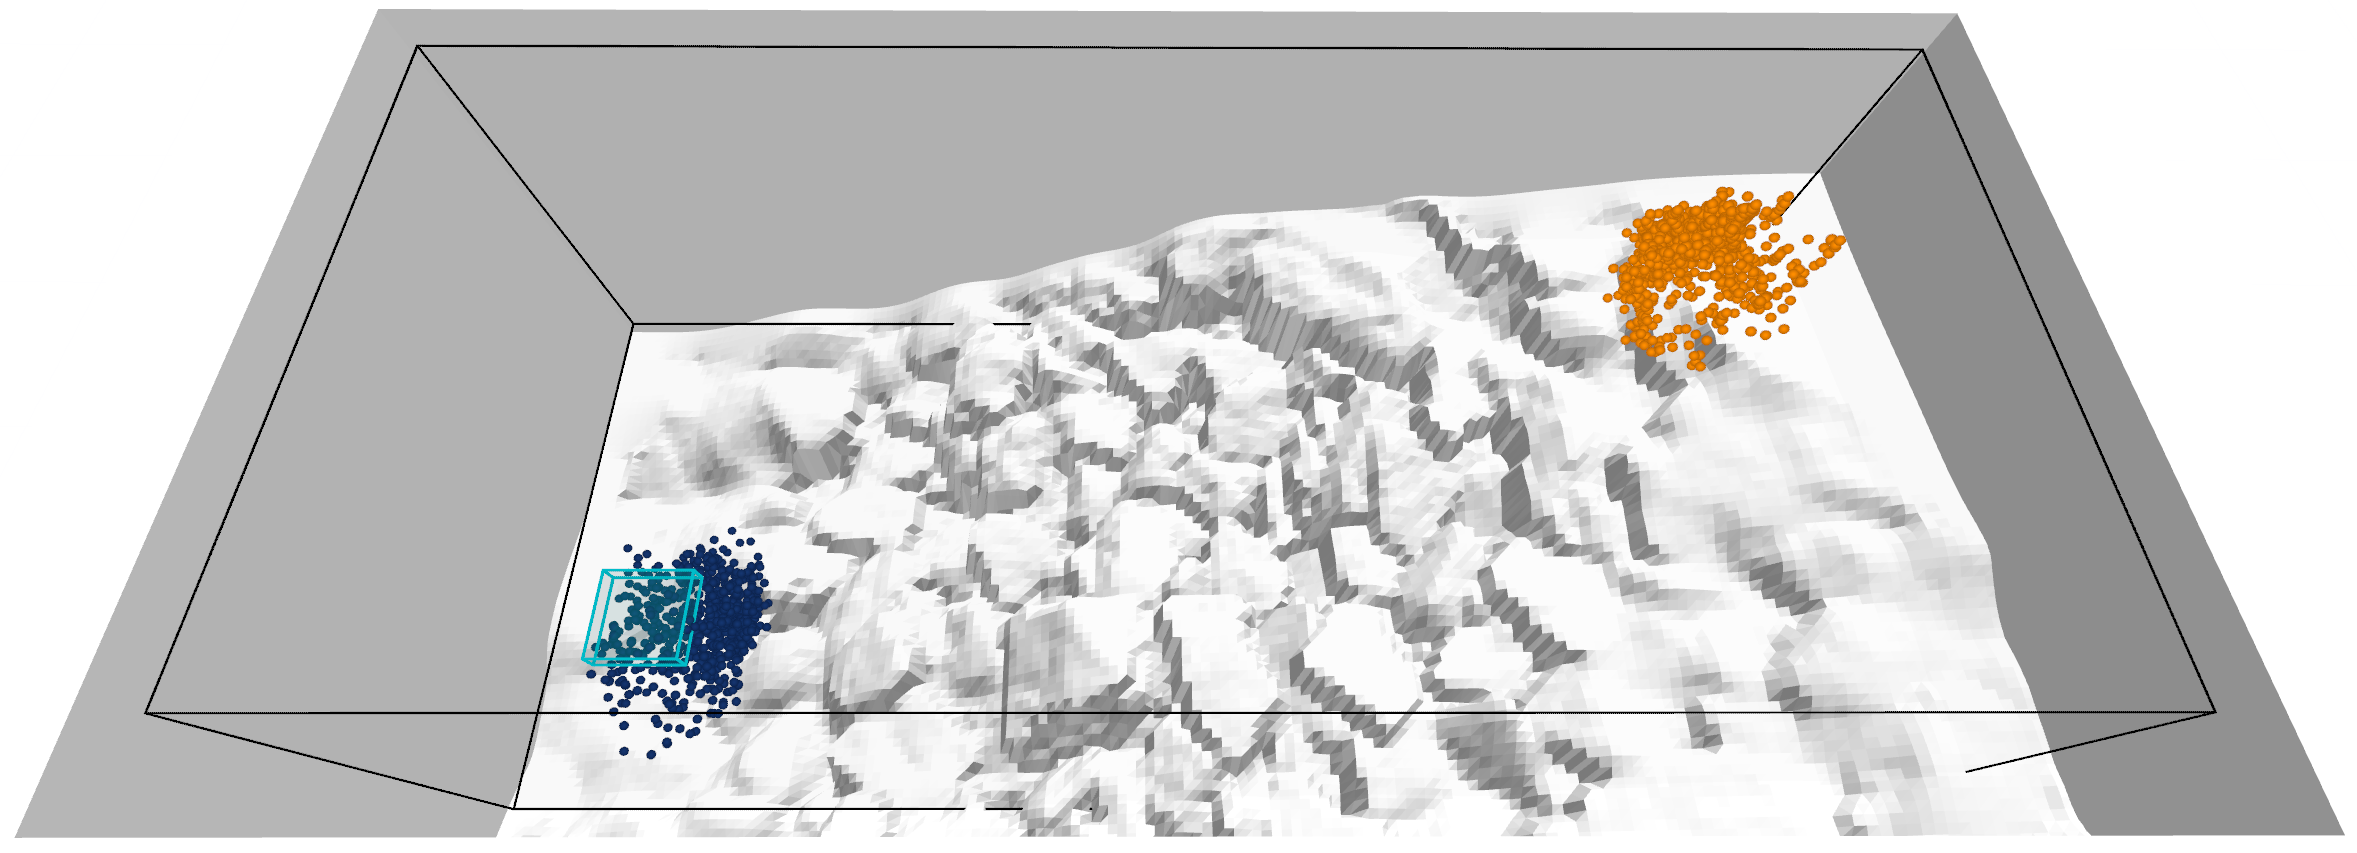
\includegraphics[width=\linewidth]{img/scans/ra_150.png}
        \caption{Iteration 150.}\label{fig:ra_150}
    \end{subfigure}
    \hfill
    \begin{subfigure}[t]{0.24\linewidth}
        \centering
        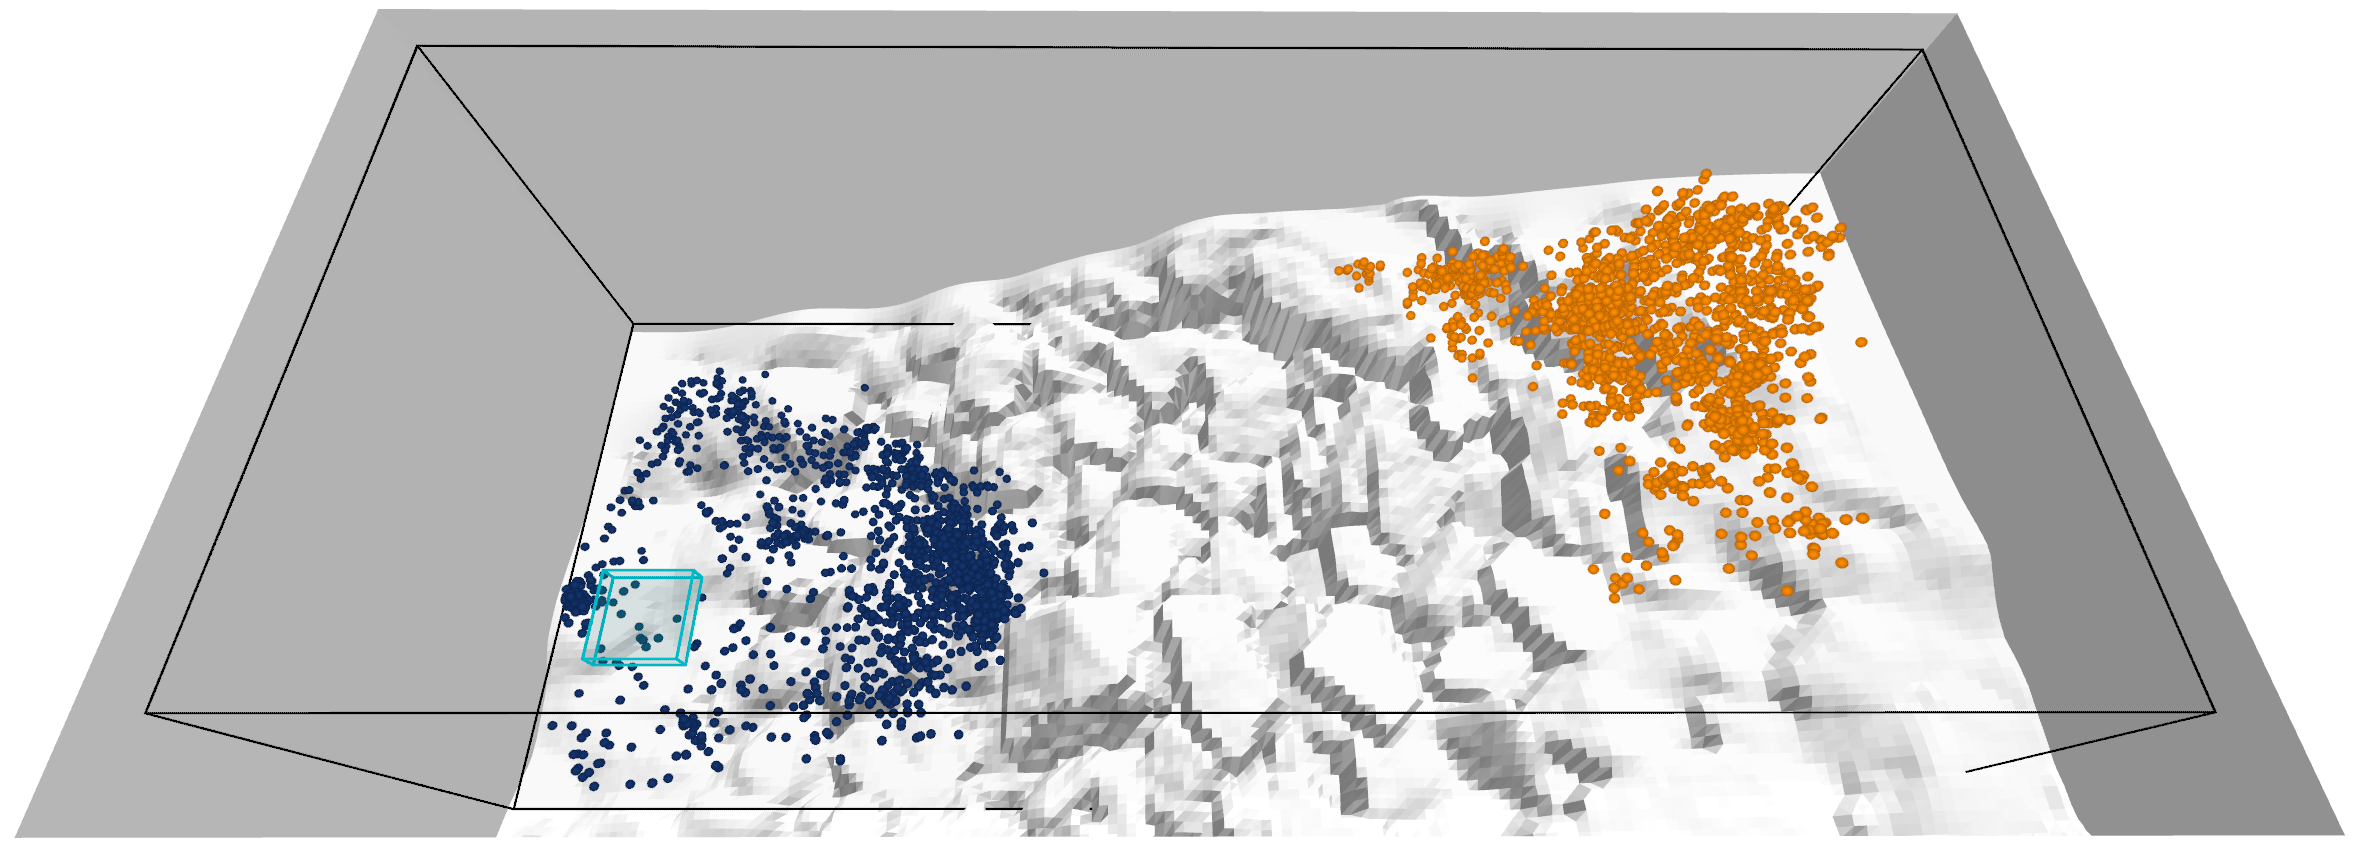
\includegraphics[width=\linewidth]{img/scans/ra_500.png}
        \caption{Iteration 500.}\label{fig:ra_500}
    \end{subfigure}
    \hfill
    \begin{subfigure}[t]{0.24\linewidth}
        \centering
        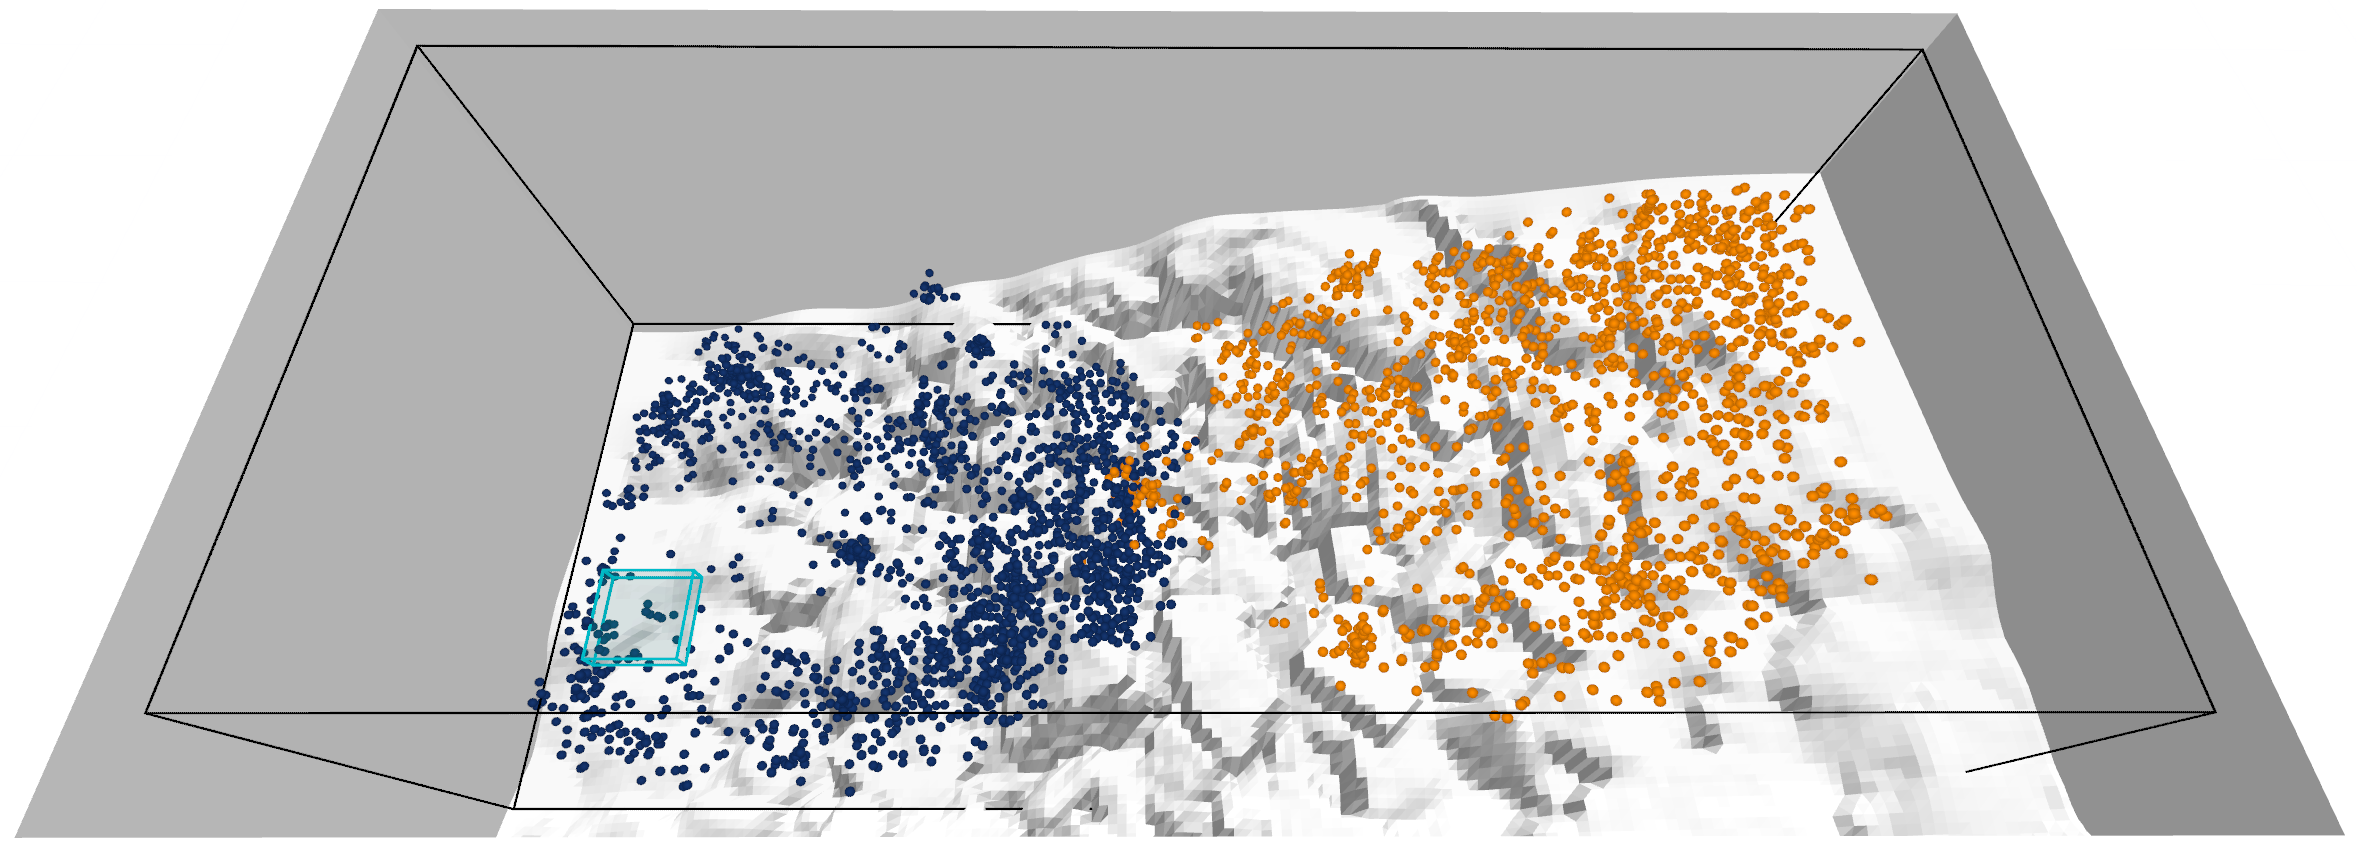
\includegraphics[width=\linewidth]{img/scans/ra_1000.png}
        \caption{Iteration 1000.}\label{fig:ra_1000}
    \end{subfigure}
    \hfill
    \begin{subfigure}[t]{0.24\linewidth}
        \centering
        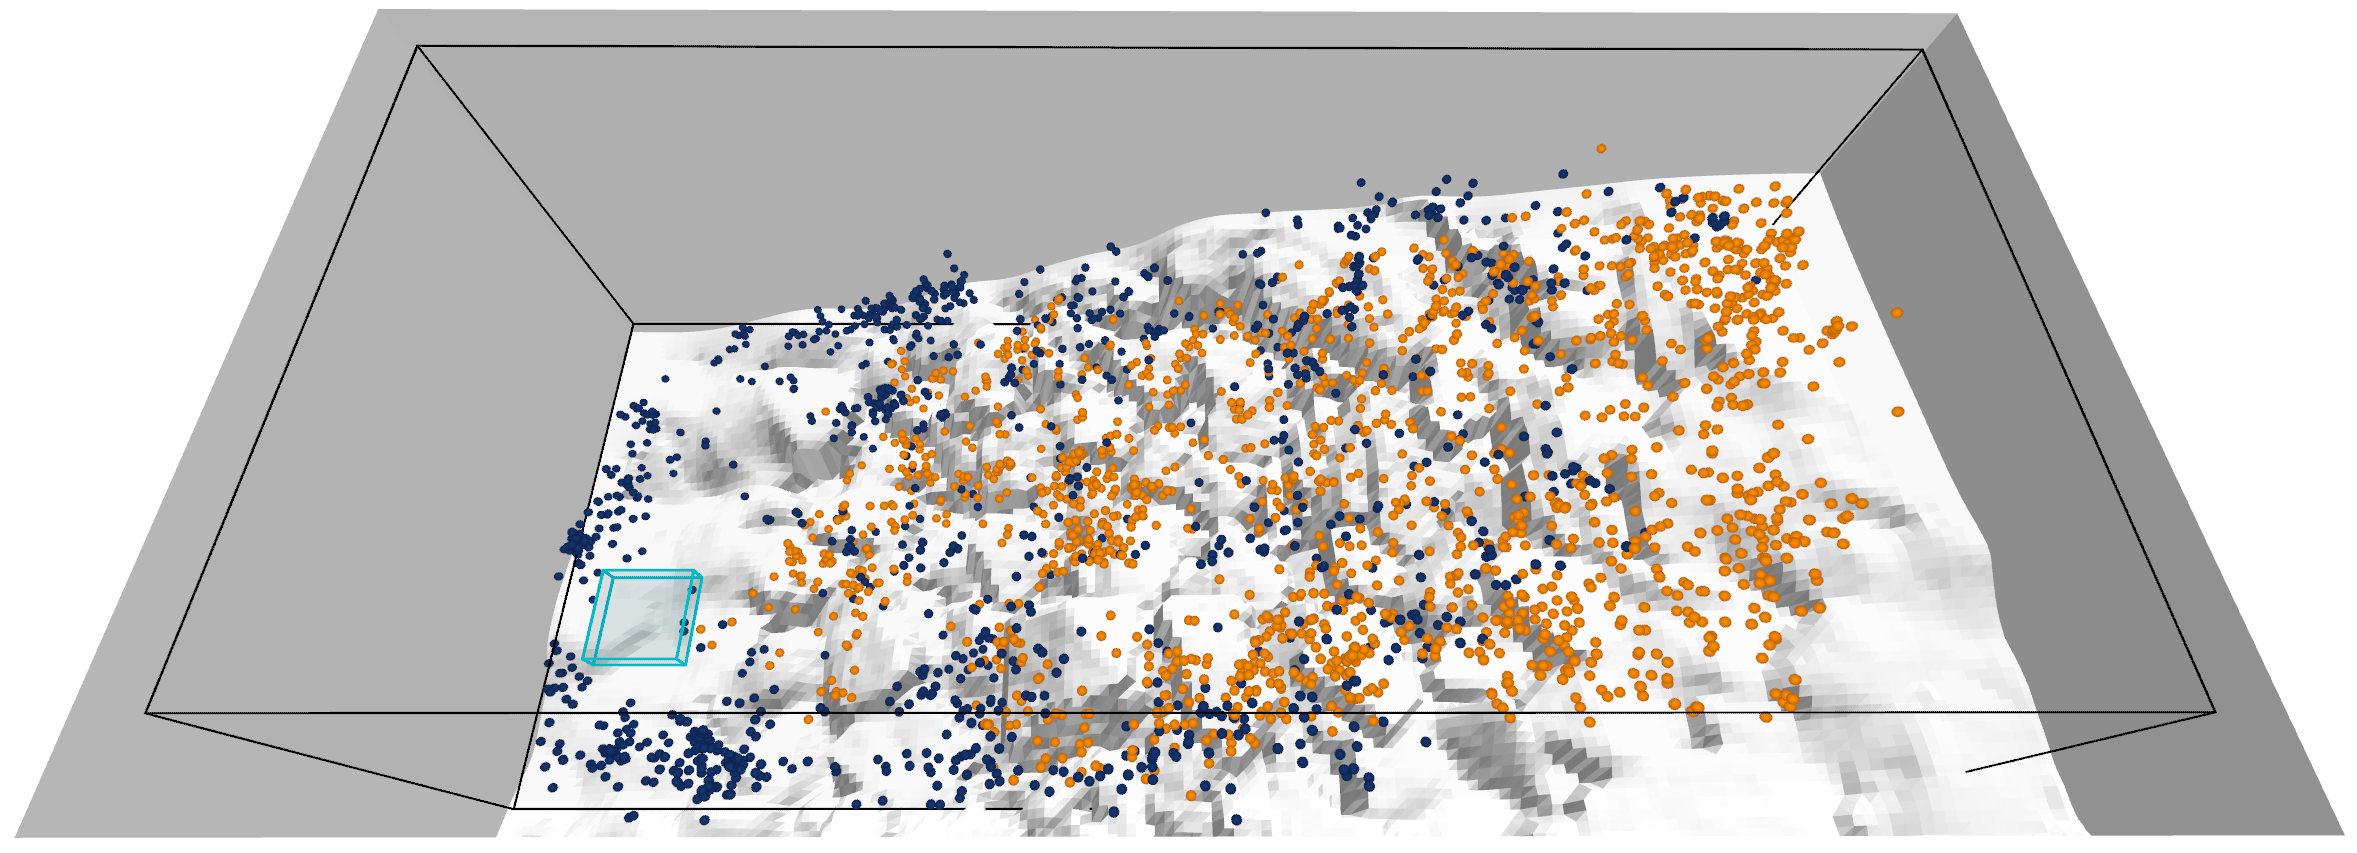
\includegraphics[width=\linewidth]{img/scans/ra_2000.png}
        \caption{Iteration 2000.}\label{fig:ra_2000}
    \end{subfigure}
    \hfill\strut{}
    \caption{Samples of the explored regions on the \textit{rocky ascent} terrain at different training iterations. {\color{blue} Blue} indicates the intermediate goals (forwards expansion), {\color{orange} orange} indicates the intermediate starts (backwards expansion), {\color{cyan}cyan} indicates the initial distribution, and the black/white box represents the task space.}\label{fig:scans}
\end{figure}
\subsection{Generalization to Different Domains: Manipulation Tasks}\label{sec:exp_manipulation}

todo
\begin{wrapfigure}{r}{0.24\linewidth}
    \centering
    \vspace{-\baselineskip}
    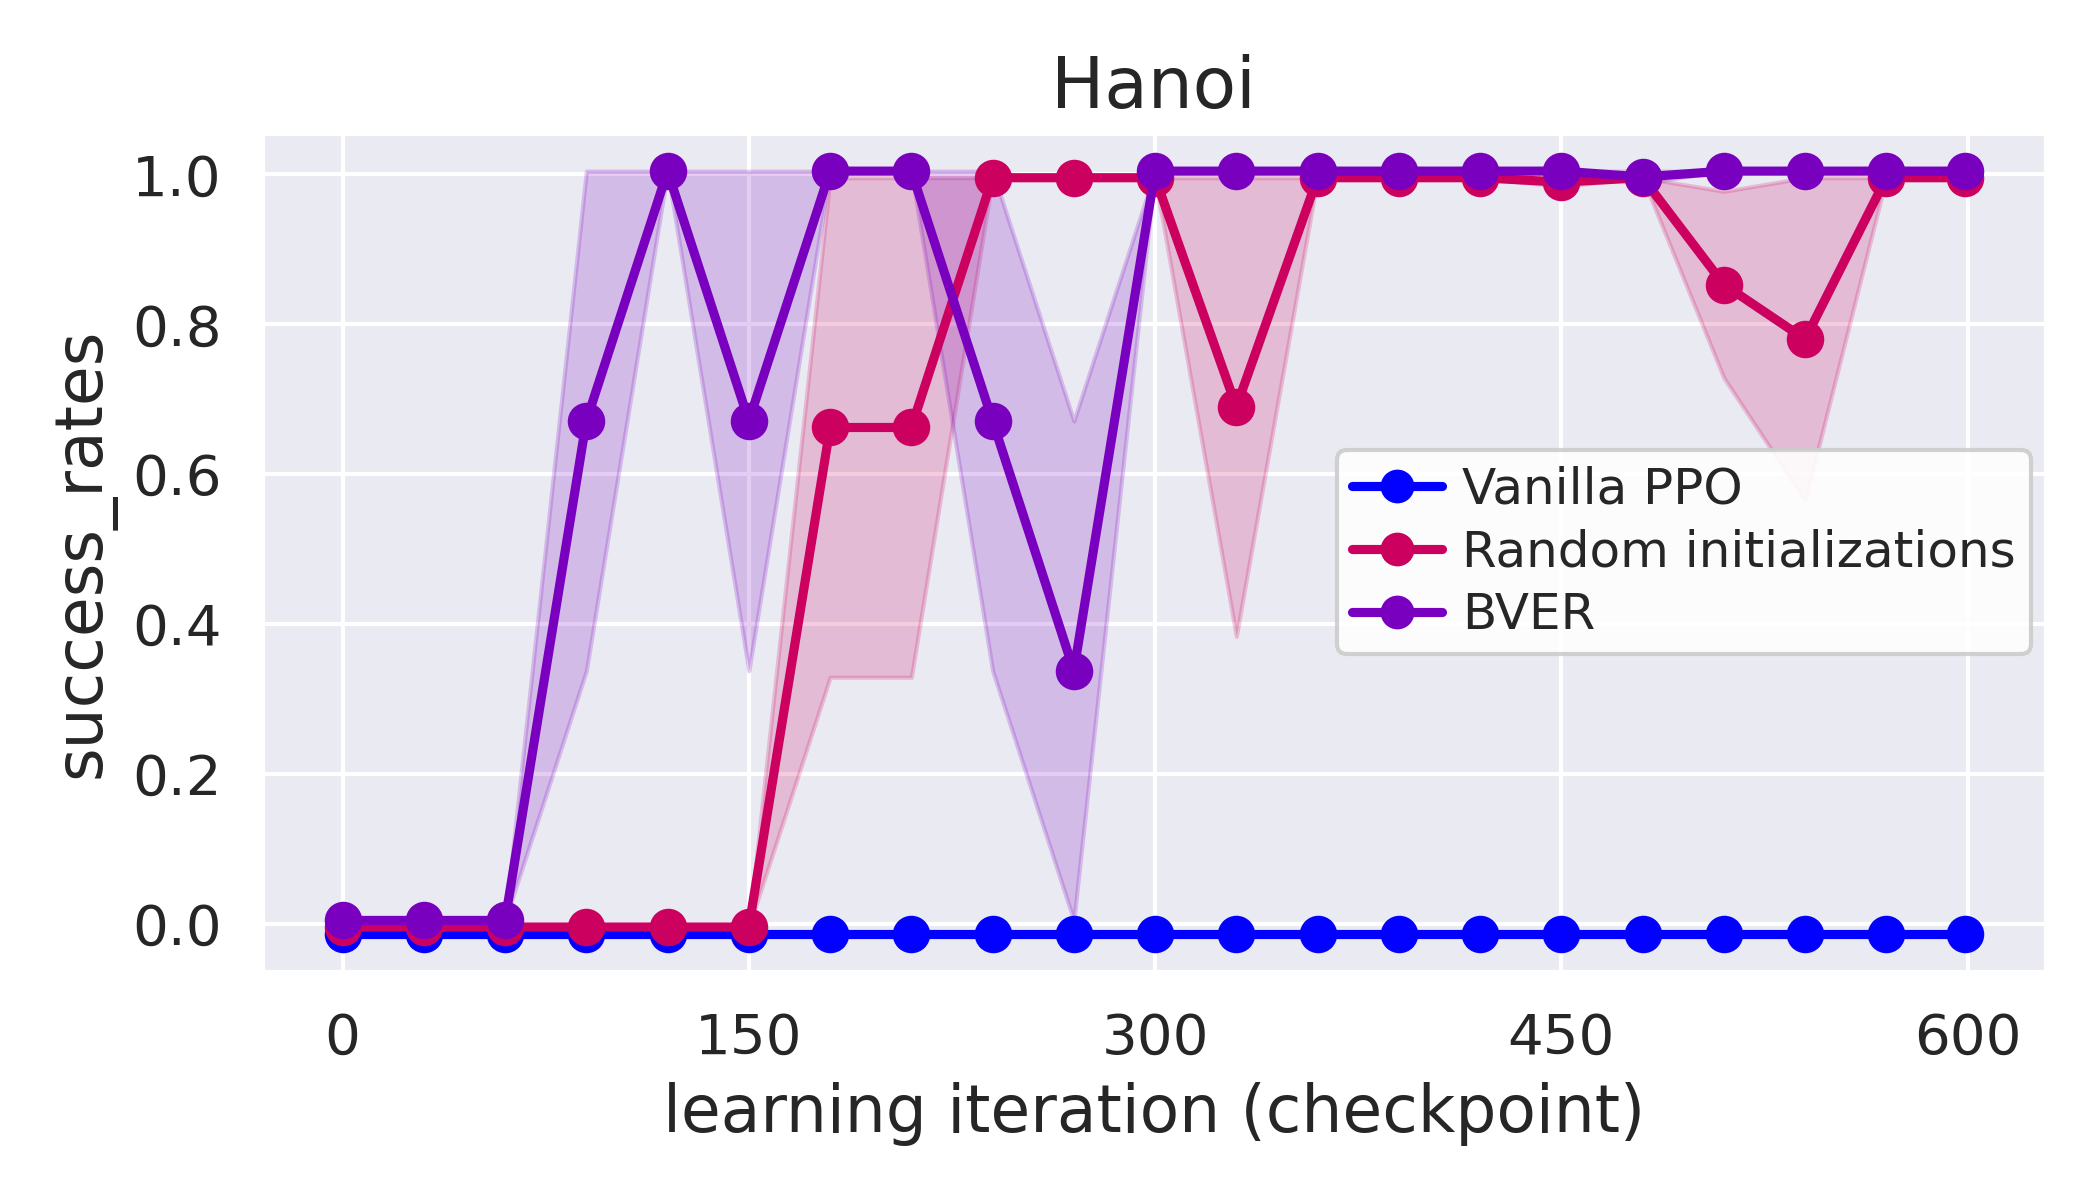
\includegraphics[width=\linewidth]{img/manipulation/eval_comparison_hanoi_bench.png}
    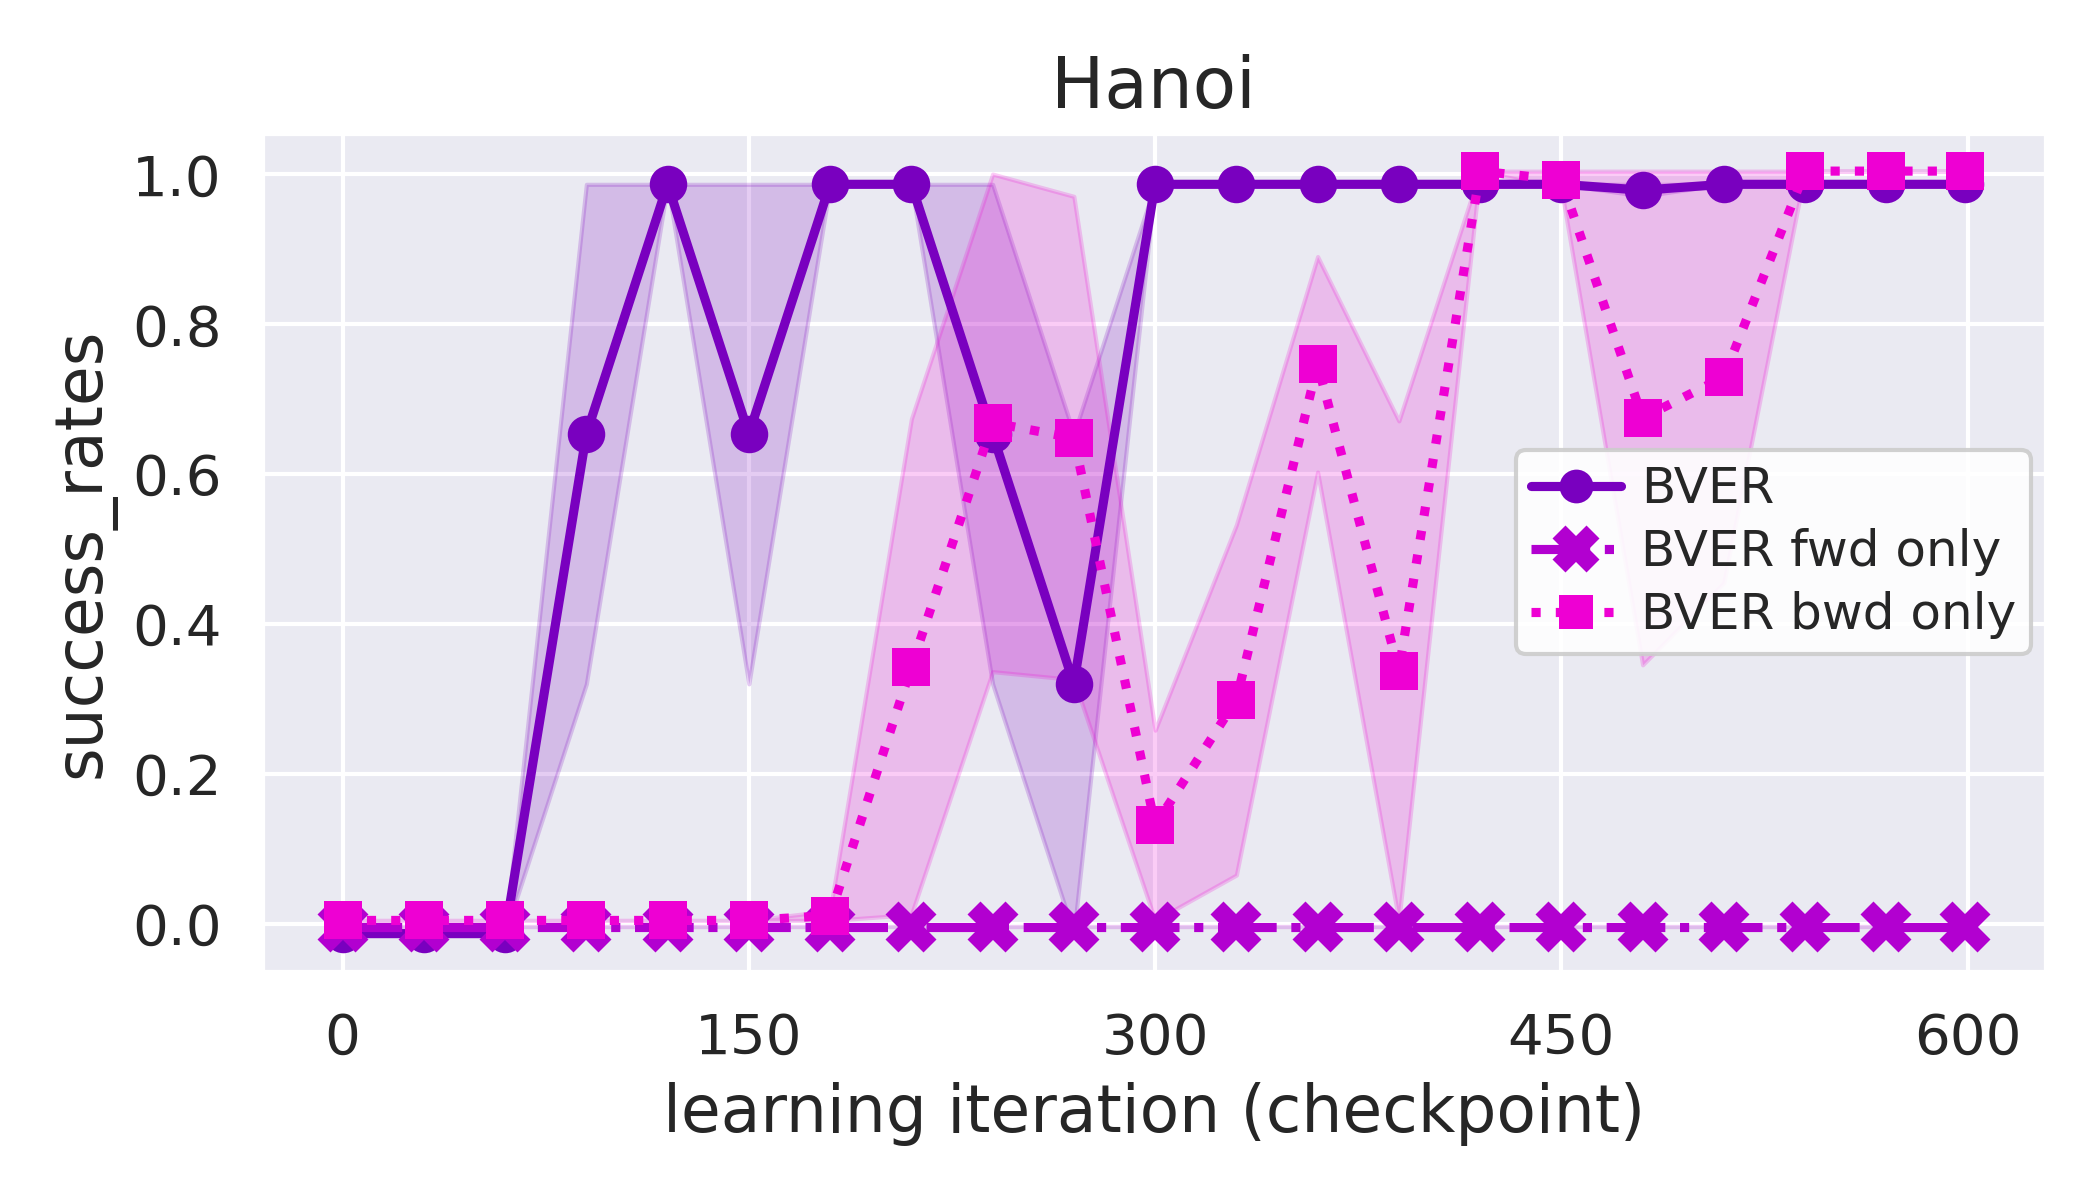
\includegraphics[width=\linewidth]{img/manipulation/eval_comparison_hanoi_abl_dir.png}
    \caption{Top row shows the benchmark results, and the bottom row shows the ablation results.}\label{fig:hanoi_p12}
\end{wrapfigure}
\section{Conclusion}\label{sec:conclusion}

We propose a method that combines both start-state and goal curricula for sparse-reward, long-horizon goal-conditioned reinforcement learning. We transfer the idea of bidirectional expansion from classic sampling-based planning~\citep{lavalle2001randomized, kuffner2000rrt} to curriculum generation, growing a set of start states outward from the goal and a set of goals outward from the initial state distribution, biasing both toward unexplored regions of the task space, and steering the two frontiers toward each other. Experimental results show that this leads to sample-efficient and robust policies on quadrupedal box climbing, real-world terrains, point-mass mazes, and manipulation tasks. Furthermore, our approach adds minimal computational overhead and thus does not require excessive training time.

Our method relies on a simulator that can be reset to arbitrary states, on rollouts of random actions, and on a bounded task space with a meaningful distance metric. For the latter, we rely on a Euclidean distance metric in this work, but future work could extend to or even learn different distance metrics, for example the observed number of time steps between two states proposed by~\citet{hartikainen2020dynamicaldistancelearningsemisupervised}. Instead of using random walk rollouts to estimate the reachability of states, future work could also explore the use of learned dynamics models or using the current policy to roll out trajectories.



\subsubsection*{Reproducibility statement}
% Optional; does not count toward the page limit.
% TODO Describe the efforts made to ensure reproducibility (code, seeds,
% hyperparameters, hardware), or remove this block.

% Author contributions and acknowledgements reveal identity: keep them commented
% out for the double-blind submission, uncomment for the camera-ready version
% (together with \iclrfinalcopy).
%\subsubsection*{Author contributions}
% TODO

%\subsubsection*{Acknowledgements}
% TODO Funding acknowledgements go here (not in the author footnote).

\bibliography{references}
\bibliographystyle{iclr2026_conference}

\appendix
\section{Appendix}\label{sec:appendix}

% Appendices do not count toward the page limit.
\begin{figure}[h]
    \centering
    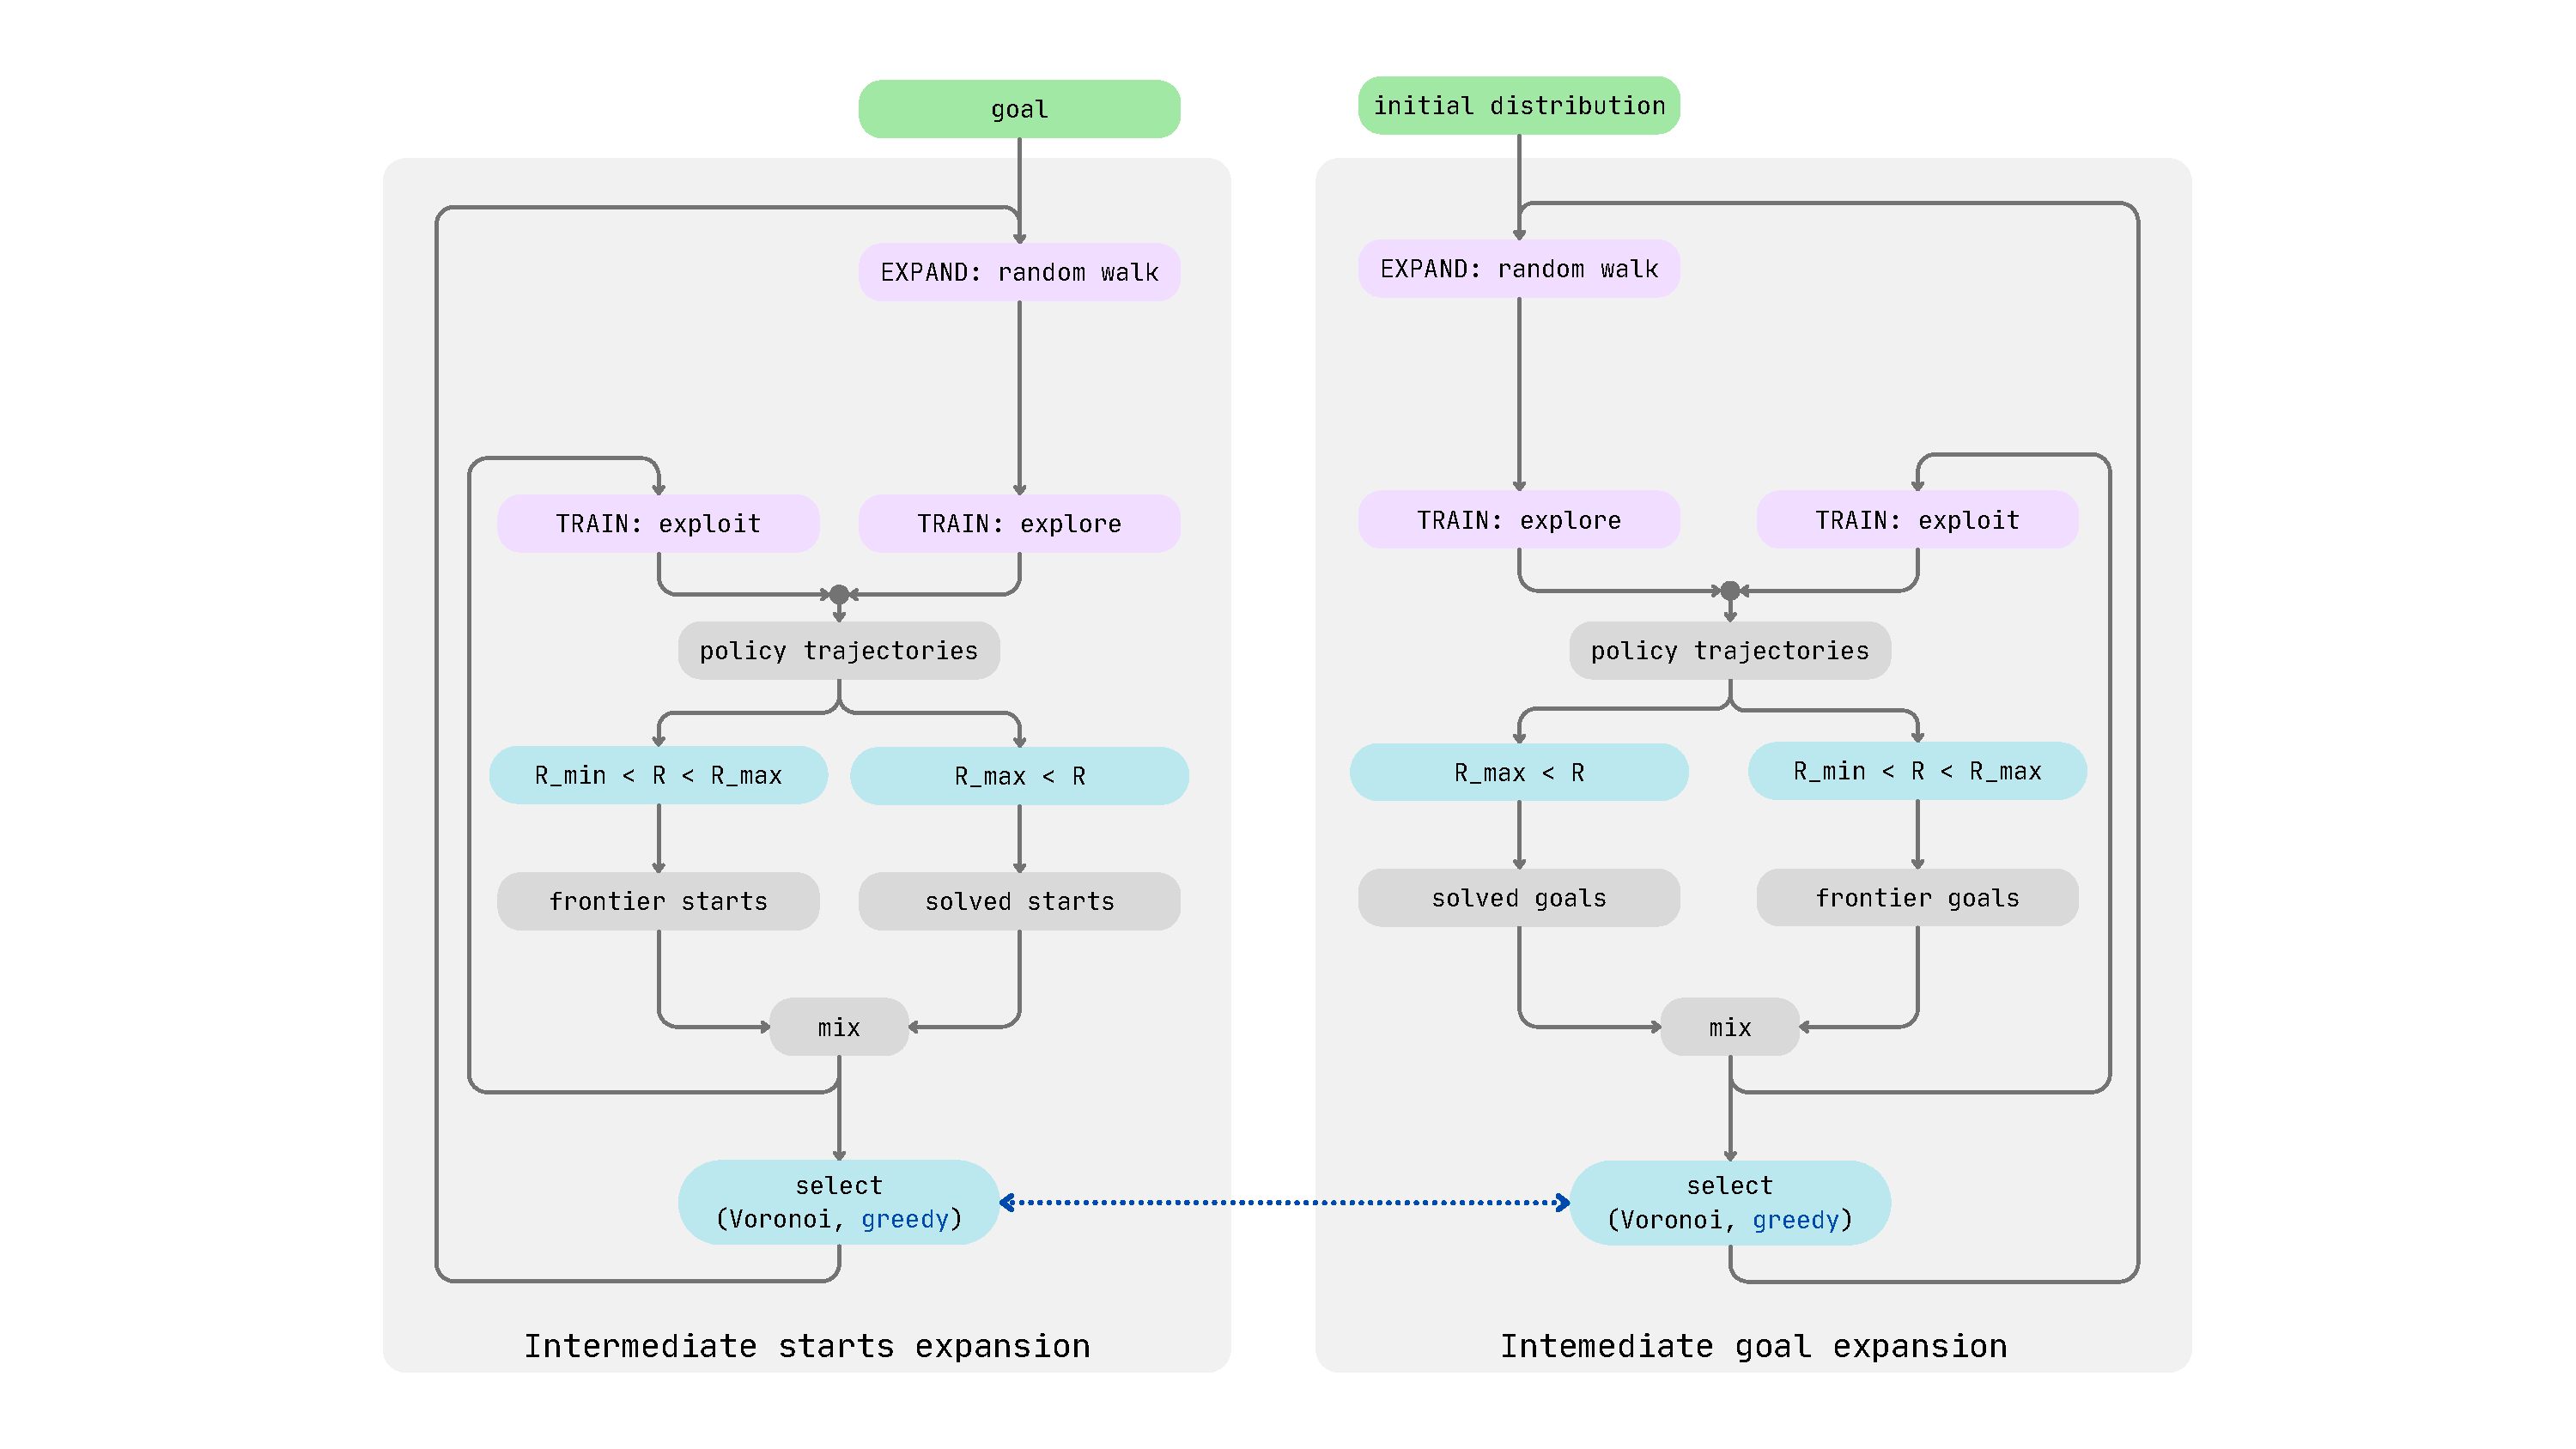
\includegraphics[width=\linewidth]{img/graphics/scheme_full.pdf}
    \caption{Overview of BVER. Both expansions run the same loop: random walks seeded in the goal (left) or the initial distribution (right) propose new starts or goals (explore), which are trained on together with the mixed training set (exploit). Rollout returns $R$ split the trained states into frontier ($R_{\min} < R < R_{\max}$) and solved ($R_{\max} \leq R$) states, which are mixed into the next training set. The seeds of the next random walks are selected from this set by nearest neighbors to uniform samples of the task space (Voronoi bias) or to states of the other expansion (connect step, dotted arrow).}\label{fig:method}
\end{figure}

\subsection{Simulation setup}\label{sec:appendix_obs_act}
% TODO: observation and action spaces, simulation and PPO hyperparameters.


\end{document}
